%%
%% Automatically generated file from DocOnce source
%% (https://github.com/hplgit/doconce/)
%%

% #define PREAMBLE

% #ifdef PREAMBLE
%-------------------- begin preamble ----------------------

\documentclass[%
oneside,                 % oneside: electronic viewing, twoside: printing
final,                   % draft: marks overfull hboxes, figures with paths
10pt]{article}

\listfiles               % print all files needed to compile this document

\usepackage{relsize,makeidx,color,setspace,amsmath,amsfonts,amssymb}
\usepackage[table]{xcolor}
\usepackage{bm,microtype}

\usepackage[pdftex]{graphicx}

% Packages for typesetting blocks of computer code
\usepackage{fancyvrb,framed,moreverb}

% Define colors
\definecolor{orange}{cmyk}{0,0.4,0.8,0.2}
\definecolor{tucorange}{rgb}{1.0,0.64,0}
\definecolor{darkorange}{rgb}{.71,0.21,0.01}
\definecolor{darkgreen}{rgb}{.12,.54,.11}
\definecolor{myteal}{rgb}{.26, .44, .56}
\definecolor{gray}{gray}{0.45}
\definecolor{mediumgray}{gray}{.8}
\definecolor{lightgray}{gray}{.95}
\definecolor{brown}{rgb}{0.54,0.27,0.07}
\definecolor{purple}{rgb}{0.5,0.0,0.5}
\definecolor{darkgray}{gray}{0.25}
\definecolor{darkblue}{rgb}{0,0.08,0.45}
\definecolor{darkblue2}{rgb}{0,0,0.8}
\definecolor{lightred}{rgb}{1.0,0.39,0.28}
\definecolor{lightgreen}{rgb}{0.48,0.99,0.0}
\definecolor{lightblue}{rgb}{0.53,0.81,0.92}
\definecolor{lightblue2}{rgb}{0.3,0.3,1.0}
\definecolor{lightpurple}{rgb}{0.87,0.63,0.87}
\definecolor{lightcyan}{rgb}{0.5,1.0,0.83}

\colorlet{comment_green}{green!50!black}
\colorlet{string_red}{red!60!black}
\colorlet{keyword_pink}{magenta!70!black}
\colorlet{indendifier_green}{green!70!white}

% Backgrounds for code
\definecolor{cbg_gray}{rgb}{.95, .95, .95}
\definecolor{bar_gray}{rgb}{.92, .92, .92}

\definecolor{cbg_yellowgray}{rgb}{.95, .95, .85}
\definecolor{bar_yellowgray}{rgb}{.95, .95, .65}

\colorlet{cbg_yellow2}{yellow!10}
\colorlet{bar_yellow2}{yellow!20}

\definecolor{cbg_yellow1}{rgb}{.98, .98, 0.8}
\definecolor{bar_yellow1}{rgb}{.98, .98, 0.4}

\definecolor{cbg_red1}{rgb}{1, 0.85, 0.85}
\definecolor{bar_red1}{rgb}{1, 0.75, 0.85}

\definecolor{cbg_blue1}{rgb}{0.87843, 0.95686, 1.0}
\definecolor{bar_blue1}{rgb}{0.7,     0.95686, 1}

%\setlength{\fboxsep}{-1.5mm}  % adjust cod_vpad/pro_vpad background box

%% Background for code blocks (parameter is color name)

%% pro/cod_vpad: gives some vertical padding before and after the text
%% (but has more simplistic code than _cod/pro_tight+cod/pro).
%% pro/cod_vpad can be used to enclose Verbatim or lst begin/end for code.
%% pro/cod calls _pro/cod_tight and has very little vertical padding,
%% used to enclose Verbatim and other begin/end for code.
%% (pro/cod is what the ptex2tex program could produce with the
%% Blue/BlueBar definitions in .ptex2tex.cfg.)

\newenvironment{cod_vpad}[1]{
   \def\FrameCommand{\colorbox{#1}}
   \MakeFramed{\FrameRestore}}
   {\endMakeFramed}

\newenvironment{_cod_tight}[1]{
   \def\FrameCommand{\colorbox{#1}}
   \FrameRule0.6pt\MakeFramed {\FrameRestore}\vskip3mm}
   {\vskip0mm\endMakeFramed}

\newenvironment{cod}[1]{
\bgroup\rmfamily
\fboxsep=0mm\relax
\begin{_cod_tight}{#1}
\list{}{\parsep=-2mm\parskip=0mm\topsep=0pt\leftmargin=2mm
\rightmargin=2\leftmargin\leftmargin=4pt\relax}
\item\relax}
{\endlist\end{_cod_tight}\egroup}

%% Background for complete program blocks (parameter 1 is color name
%% for background, parameter 2 is color for left bar)
\newenvironment{pro_vpad}[2]{
   \def\FrameCommand{\color{#2}\vrule width 1mm\normalcolor\colorbox{#1}}
   \MakeFramed{\FrameRestore}}
   {\endMakeFramed}

\newenvironment{_pro_tight}[2]{
   \def\FrameCommand{\color{#2}\vrule width 1mm\normalcolor\colorbox{#1}}
   \FrameRule0.6pt\MakeFramed {\advance\hsize-2mm\FrameRestore}\vskip3mm}
   {\vskip0mm\endMakeFramed}

\newenvironment{pro}[2]{
\bgroup\rmfamily
\fboxsep=0mm\relax
\begin{_pro_tight}{#1}{#2}
\list{}{\parsep=-2mm\parskip=0mm\topsep=0pt\leftmargin=2mm
\rightmargin=2\leftmargin\leftmargin=4pt\relax}
\item\relax}
{\endlist\end{_pro_tight}\egroup}


\usepackage[T1]{fontenc}
%\usepackage[latin1]{inputenc}
\usepackage{ucs}
\usepackage[utf8x]{inputenc}

\usepackage{lmodern}         % Latin Modern fonts derived from Computer Modern

% Hyperlinks in PDF:
\definecolor{linkcolor}{rgb}{0,0,0.4}
\usepackage{hyperref}
\hypersetup{
    breaklinks=true,
    colorlinks=true,
    linkcolor=linkcolor,
    urlcolor=linkcolor,
    citecolor=black,
    filecolor=black,
    %filecolor=blue,
    pdfmenubar=true,
    pdftoolbar=true,
    bookmarksdepth=3   % Uncomment (and tweak) for PDF bookmarks with more levels than the TOC
    }
%\hyperbaseurl{}   % hyperlinks are relative to this root

\setcounter{tocdepth}{2}  % number chapter, section, subsection

% Tricks for having figures close to where they are defined:
% 1. define less restrictive rules for where to put figures
\setcounter{topnumber}{2}
\setcounter{bottomnumber}{2}
\setcounter{totalnumber}{4}
\renewcommand{\topfraction}{0.95}
\renewcommand{\bottomfraction}{0.95}
\renewcommand{\textfraction}{0}
\renewcommand{\floatpagefraction}{0.75}
% floatpagefraction must always be less than topfraction!
% 2. ensure all figures are flushed before next section
\usepackage[section]{placeins}
% 3. enable begin{figure}[H] (often leads to ugly pagebreaks)
%\usepackage{float}\restylefloat{figure}

% newcommands for typesetting inline (doconce) comments
\newcommand{\shortinlinecomment}[3]{{\color{red}{\bf #1}: #2}}
\newcommand{\longinlinecomment}[3]{{\color{red}{\bf #1}: #2}}

\usepackage[framemethod=TikZ]{mdframed}

% --- begin definitions of admonition environments ---

% Admonition style "mdfbox" is an oval colored box based on mdframed
% "notice" admon
\colorlet{mdfbox_notice_background}{gray!5}
\newmdenv[
  skipabove=15pt,
  skipbelow=15pt,
  outerlinewidth=0,
  backgroundcolor=mdfbox_notice_background,
  linecolor=black,
  linewidth=2pt,       % frame thickness
  frametitlebackgroundcolor=blue!5,
  frametitlerule=true,
  frametitlefont=\normalfont\bfseries,
  shadow=false,        % frame shadow?
  shadowsize=11pt,
  leftmargin=0,
  rightmargin=0,
  roundcorner=5,
  needspace=0pt,
]{notice_mdfboxmdframed}

\newenvironment{notice_mdfboxadmon}[1][]{
\begin{notice_mdfboxmdframed}[frametitle=#1]
}
{
\end{notice_mdfboxmdframed}
}

% Admonition style "mdfbox" is an oval colored box based on mdframed
% "summary" admon
\colorlet{mdfbox_summary_background}{gray!5}
\newmdenv[
  skipabove=15pt,
  skipbelow=15pt,
  outerlinewidth=0,
  backgroundcolor=mdfbox_summary_background,
  linecolor=black,
  linewidth=2pt,       % frame thickness
  frametitlebackgroundcolor=blue!5,
  frametitlerule=true,
  frametitlefont=\normalfont\bfseries,
  shadow=false,        % frame shadow?
  shadowsize=11pt,
  leftmargin=0,
  rightmargin=0,
  roundcorner=5,
  needspace=0pt,
]{summary_mdfboxmdframed}

\newenvironment{summary_mdfboxadmon}[1][]{
\begin{summary_mdfboxmdframed}[frametitle=#1]
}
{
\end{summary_mdfboxmdframed}
}

% Admonition style "mdfbox" is an oval colored box based on mdframed
% "warning" admon
\colorlet{mdfbox_warning_background}{gray!5}
\newmdenv[
  skipabove=15pt,
  skipbelow=15pt,
  outerlinewidth=0,
  backgroundcolor=mdfbox_warning_background,
  linecolor=black,
  linewidth=2pt,       % frame thickness
  frametitlebackgroundcolor=blue!5,
  frametitlerule=true,
  frametitlefont=\normalfont\bfseries,
  shadow=false,        % frame shadow?
  shadowsize=11pt,
  leftmargin=0,
  rightmargin=0,
  roundcorner=5,
  needspace=0pt,
]{warning_mdfboxmdframed}

\newenvironment{warning_mdfboxadmon}[1][]{
\begin{warning_mdfboxmdframed}[frametitle=#1]
}
{
\end{warning_mdfboxmdframed}
}

% Admonition style "mdfbox" is an oval colored box based on mdframed
% "question" admon
\colorlet{mdfbox_question_background}{gray!5}
\newmdenv[
  skipabove=15pt,
  skipbelow=15pt,
  outerlinewidth=0,
  backgroundcolor=mdfbox_question_background,
  linecolor=black,
  linewidth=2pt,       % frame thickness
  frametitlebackgroundcolor=blue!5,
  frametitlerule=true,
  frametitlefont=\normalfont\bfseries,
  shadow=false,        % frame shadow?
  shadowsize=11pt,
  leftmargin=0,
  rightmargin=0,
  roundcorner=5,
  needspace=0pt,
]{question_mdfboxmdframed}

\newenvironment{question_mdfboxadmon}[1][]{
\begin{question_mdfboxmdframed}[frametitle=#1]
}
{
\end{question_mdfboxmdframed}
}

% Admonition style "mdfbox" is an oval colored box based on mdframed
% "block" admon
\colorlet{mdfbox_block_background}{gray!5}
\newmdenv[
  skipabove=15pt,
  skipbelow=15pt,
  outerlinewidth=0,
  backgroundcolor=mdfbox_block_background,
  linecolor=black,
  linewidth=2pt,       % frame thickness
  frametitlebackgroundcolor=blue!5,
  frametitlerule=true,
  frametitlefont=\normalfont\bfseries,
  shadow=false,        % frame shadow?
  shadowsize=11pt,
  leftmargin=0,
  rightmargin=0,
  roundcorner=5,
  needspace=0pt,
]{block_mdfboxmdframed}

\newenvironment{block_mdfboxadmon}[1][]{
\begin{block_mdfboxmdframed}[frametitle=#1]
}
{
\end{block_mdfboxmdframed}
}

% --- end of definitions of admonition environments ---

% prevent orhpans and widows
\clubpenalty = 10000
\widowpenalty = 10000

\newenvironment{doconceexercise}{}{}
\newcounter{doconceexercisecounter}
% --- begin definition of \listofexercises command ---
\makeatletter
\newcommand\listofexercises{\section*{List of Exercises and Problems}
\@starttoc{loe}
}
\newcommand*{\l@doconceexercise}{\@dottedtocline{0}{0pt}{6.5em}}
\makeatother
% --- end definition of \listofexercises command ---



% ------ header in subexercises ------
%\newcommand{\subex}[1]{\paragraph{#1}}
%\newcommand{\subex}[1]{\par\vspace{1.7mm}\noindent{\bf #1}\ \ }
\makeatletter
% 1.5ex is the spacing above the header, 0.5em the spacing after subex title
\newcommand\subex{\@startsection{paragraph}{4}{\z@}%
                  {1.5ex\@plus1ex \@minus.2ex}%
                  {-0.5em}%
                  {\normalfont\normalsize\bfseries}}
\makeatother


% --- end of standard preamble for documents ---




% References to labels in external documents:
\usepackage{xr}
\externaldocument{/home/hpl/vc/decay-book/doc/.src/book/book}

% insert custom LaTeX commands...


\raggedbottom
\makeindex
\usepackage[totoc]{idxlayout}   % for index in the toc
\usepackage[nottoc]{tocbibind}  % for references/bibliography in the toc

%-------------------- end preamble ----------------------

\begin{document}

% matching end for #ifdef PREAMBLE
% #endif

\newcommand{\half}{\frac{1}{2}}
\newcommand{\halfi}{{1/2}}
\newcommand{\tp}{\thinspace .}

\newcommand{\uex}{u_{\mbox{\footnotesize e}}}
\newcommand{\uexd}[1]{u_{\mbox{\footnotesize e}, #1}}
\newcommand{\vex}{v_{\mbox{\footnotesize e}}}
\newcommand{\Vex}{V_{\mbox{\footnotesize e}}}
\newcommand{\vexd}[1]{v_{\mbox{\footnotesize e}, #1}}
\newcommand{\Aex}{A_{\mbox{\footnotesize e}}}

% Operators
\newcommand{\Ddt}[1]{\frac{D #1}{dt}}
\newcommand{\E}[1]{\hbox{E}\lbrack #1 \rbrack}
\newcommand{\Var}[1]{\hbox{Var}\lbrack #1 \rbrack}
\newcommand{\Std}[1]{\hbox{Std}\lbrack #1 \rbrack}

\newcommand{\xpoint}{\bm{x}}
\newcommand{\normalvec}{\bm{n}}
\newcommand{\Oof}[1]{\mathcal{O}(#1)}

% Boldface vectors/tensors
\newcommand{\x}{\bm{x}}
\newcommand{\X}{\bm{X}}
\renewcommand{\u}{\bm{u}}
\renewcommand{\v}{\bm{v}}
\newcommand{\w}{\bm{w}}
\newcommand{\acc}{\bm{a}}
\newcommand{\rpos}{\bm{r}}
\newcommand{\V}{\bm{V}}
\newcommand{\e}{\bm{e}}
\newcommand{\f}{\bm{f}}
\newcommand{\F}{\bm{F}}
\newcommand{\stress}{\bm{\sigma}}
\newcommand{\strain}{\bm{\varepsilon}}
\newcommand{\stressc}{{\sigma}}
\newcommand{\strainc}{{\varepsilon}}
\newcommand{\I}{\bm{I}}
\newcommand{\T}{\bm{T}}
\newcommand{\U}{\bm{U}}

\newcommand{\dfc}{\alpha}  % diffusion coefficient
% Unit vectors
\newcommand{\ii}{\bm{i}}
\newcommand{\jj}{\bm{j}}
\newcommand{\kk}{\bm{k}}
\newcommand{\ir}{\bm{i}_r}
\newcommand{\ith}{\bm{i}_{\theta}}
\newcommand{\iz}{\bm{i}_z}

% Index sets
\newcommand{\Ix}{\mathcal{I}_x}
\newcommand{\Iy}{\mathcal{I}_y}
\newcommand{\Iz}{\mathcal{I}_z}
\newcommand{\It}{\mathcal{I}_t}
%\newcommand{\Ix}{{I_x}}
%\newcommand{\Iy}{{I_y}}
%\newcommand{\Iz}{{I_z}}
%\newcommand{\It}{{I_t}}
%\newcommand{\If}{\mathcal{I}}     % for FEM
\newcommand{\If}{\mathcal{I}_s}     % for FEM
%\newcommand{\If}{{I}}     % for FEM
%\newcommand{\Ifd}{\mathcal{I}_d}  % for FEM
\newcommand{\Ifd}{{I_d}}  % for FEM
\newcommand{\Ifb}{{I_b}}  % for FEM
\newcommand{\setb}[1]{#1^0}    % set begin
\newcommand{\sete}[1]{#1^{-1}} % set end
%\newcommand{\setl}[1]{#1\setminus\{\set1{#1}\}}
%\newcommand{\setr}[1]{#1\setminus\{\set0{#1}\}}
%\newcommand{\seti}[1]{#1\setminus\{\set0{#1},\set1{#1}\}}
\newcommand{\setl}[1]{#1^-}
\newcommand{\setr}[1]{#1^+}
\newcommand{\seti}[1]{#1^i}
\newcommand{\sequencei}[1]{\left\{ {#1}_i \right\}_{i\in\If}}
\newcommand{\sequencej}[1]{\left\{ {#1}_j \right\}_{j\in\If}}

% Finite elements
\newcommand{\basphi}{\varphi}
\newcommand{\baspsi}{\psi}
\newcommand{\refphi}{\tilde\basphi}
\newcommand{\psib}{\bm{\psi}}
\newcommand{\sinL}[1]{\sin\left((#1+1)\pi\frac{x}{L}\right)}
\newcommand{\xno}[1]{x_{#1}}
%\newcommand{\xno}[1]{x^{(#1)}}
\newcommand{\Xno}[1]{X_{(#1)}}
\newcommand{\yno}[1]{y_{#1}}
\newcommand{\Yno}[1]{Y_{(#1)}}
\newcommand{\xdno}[1]{\bm{x}_{#1}}

% FEniCS commands
\newcommand{\dX}{\, \mathrm{d}X}
\newcommand{\dx}{\, \mathrm{d}x}
\newcommand{\ds}{\, \mathrm{d}s}
\newcommand{\Real}{\mathbb{R}}
\newcommand{\Integerp}{\mathbb{N}}
\newcommand{\Integer}{\mathbb{Z}}


% ------------------- main content ----------------------



% ----------------- title -------------------------

\thispagestyle{empty}

\begin{center}
{\LARGE\bf
\begin{spacing}{1.25}
Finite difference methods for vibration problems
\end{spacing}
}
\end{center}

% ----------------- author(s) -------------------------

\begin{center}
{\bf Hans Petter Langtangen${}^{1, 2}$} \\ [0mm]
\end{center}

\begin{center}
% List of all institutions:
\centerline{{\small ${}^1$Center for Biomedical Computing, Simula Research Laboratory}}
\centerline{{\small ${}^2$Department of Informatics, University of Oslo}}
\end{center}
    
% ----------------- end author(s) -------------------------

% --- begin date ---
\begin{center}
Oct 18, 2015
\end{center}
% --- end date ---

\vspace{1cm}


% Externaldocuments: /home/hpl/vc/decay-book/doc/.src/book/book





% Note: \textbf{PRELIMINARY VERSION} (expect typos)

% !split


\tableofcontents

\clearpage % pagebreak before list of exercises
\subsection*{List of Exercises and Problems}
\begin{tabular}{lrll}
Problem & 1 & Use linear/quadratic functions for verification ... & p.~\pageref{vib:exer:undamped:verify:linquad} \\
Exercise & 2 & Show linear growth of the phase with time & p.~\pageref{vib:exer:phase:err:growth} \\
Exercise & 3 & Improve the accuracy by adjusting the frequency ... & p.~\pageref{vib:exer:w:adjust} \\
Exercise & 4 & See if adaptive methods improve the phase ... & p.~\pageref{vib:exer:undamped:adaptive} \\
Exercise & 5 & Use a Taylor polynomial to compute $u^1$ & p.~\pageref{vib:exer:step4b:alt} \\
Exercise & 6 & Find the largest relevant value of $\omega\Delta t$ & p.~\pageref{vib:exer:wdt:limit} \\
Exercise & 7 & Visualize the accuracy of finite differences & p.~\pageref{vib:exer:fd:exp:plot} \\
Exercise & 8 & Verify convergence rates of the error in energy ... & p.~\pageref{vib:exer:energy:convrate} \\
Exercise & 9 & Use linear/quadratic functions for verification ... & p.~\pageref{vib:exer:verify:gen:linear} \\
Exercise & 10 & Use an exact discrete solution for verification ... & p.~\pageref{vib:exer:discrete:omega} \\
Exercise & 11 & Use analytical solution for convergence rate ... & p.~\pageref{vib:exer:conv:rate} \\
Exercise & 12 & Investigate the amplitude errors of many solvers ... & p.~\pageref{vib:exer:undamped:odespy} \\
Exercise & 13 & Minimize memory usage of a vibration solver & p.~\pageref{vib:exer:memsave} \\
Exercise & 14 & Implement the solver via classes & p.~\pageref{vib:exer:gen:class} \\
Exercise & 15 & Interpret $[D_tD_t u]^n$ as a forward-backward ... & p.~\pageref{vib:exer:DtDt:asDtpDtm} \\
Exercise & 16 & Use a backward difference for the damping ... & p.~\pageref{vib:exer:quad:damping:bw} \\
Exercise & 17 & Analysis of the Euler-Cromer scheme & p.~\pageref{vib:exer:EulerCromer:analysis} \\
Exercise & 18 & Simulate resonance & p.~\pageref{vib:exer:resonance} \\
Exercise & 19 & Simulate oscillations of a sliding box & p.~\pageref{vib:exer:sliding_box} \\
Exercise & 20 & Simulate a bouncing ball & p.~\pageref{vib:exer:bouncing:ball} \\
Exercise & 21 & Simulate an elastic pendulum & p.~\pageref{vib:exer:pendulum_elastic} \\
Exercise & 22 & Simulate an elastic pendulum with air resistance ... & p.~\pageref{vib:exer:pendulum_elastic_drag} \\
\end{tabular}
% --- end of table of exercises
\clearpage % pagebreak after list of exercises




\vspace{1cm} % after toc




% !split

% 2DO:
% _undamped -> _simple everywhere
% Long time integration by adaptive RK: will that improve the
% phase error? Do experiments where we measure the wavelength
% and plot it as function of time. Can we vectorize the
% max/min pt computation?

Vibration problems lead to differential equations with solutions that
oscillate in time, typically in a damped or undamped sinusoidal
fashion.  Such solutions put certain demands on the numerical methods
compared to other phenomena whose solutions are monotone or very smooth.
Both the frequency and amplitude of the oscillations need to be
accurately handled by the numerical schemes. Most of the reasoning and
specific building blocks introduced in the forthcoming text can be
reused to construct sound methods for partial differential equations
of wave nature in multiple spatial dimensions.

\longinlinecomment{hpl 1}{ Need to discuss errors also for the damped and nonlinear models. At least the frequency errors must be illustrated here as well and investigated numerically, either in text or exercises. }{ Need to discuss errors }

\section{Finite difference discretization}
\label{vib:model1}

Many of the numerical challenges faced when computing oscillatory
solutions to ODEs and PDEs can be captured by the very simple ODE
$u^{\prime\prime} + u =0$. This ODE is thus chosen as our starting
point for method development, implementation, and analysis.

\subsection{A basic model for vibrations}

\index{vibration ODE} \index{oscillations} \index{mechanical vibrations}

A system that vibrates without damping and external forcing
can be described by the ODE problem

\begin{equation}
u^{\prime\prime} + \omega^2u = 0,\quad u(0)=I,\ u^{\prime}(0)=0,\ t\in (0,T]
\tp
\label{vib:ode1}
\end{equation}
Here, $\omega$ and $I$ are given constants.
The exact solution of (\ref{vib:ode1}) is

\index{period (of oscillations)}
\index{frequency (of oscillations)}
\index{Hz (unit)}

\begin{equation}
u(t) = I\cos (\omega t)
\tp
\label{vib:ode1:uex}
\end{equation}
That is, $u$ oscillates with constant amplitude $I$ and
angular frequency $\omega$.
The corresponding period of oscillations (i.e., the time between two
neighboring peaks in the cosine function) is $P=2\pi/\omega$.
The number of periods per second
is $f=\omega/(2\pi)$ and measured in the unit Hz.
Both $f$ and $\omega$ are referred to as frequency, but $\omega$
is more precisely named \emph{angular frequency}, measured in rad/s.

In vibrating mechanical systems modeled by (\ref{vib:ode1}), $u(t)$
very often represents a position or a displacement of a particular
point in the system. The derivative $u^{\prime}(t)$ then has the
interpretation of velocity, and $u^{\prime\prime}(t)$ is the associated
acceleration.  The model (\ref{vib:ode1}) is not only
applicable to vibrating mechanical systems, but also to oscillations
in electrical circuits.

\subsection{A centered finite difference scheme}
\label{vib:ode1:fdm}

To formulate a finite difference method for the model
problem  (\ref{vib:ode1}) we follow the four steps explained in Section~\ref{decay:schemes:FE} in \cite{Langtangen_decay}.

\index{mesh!finite differences} \index{mesh function}

\paragraph{Step 1: Discretizing the domain.}
The domain is discretized by
introducing a uniformly partitioned time mesh.
The points in the mesh are $t_n=n\Delta t$, $n=0,1,\ldots,N_t$,
where $\Delta t = T/N_t$ is the constant length of the time steps.
We introduce a mesh function $u^n$ for $n=0,1,\ldots,N_t$, which
approximates the exact solution at the mesh points. The mesh
function will be computed from algebraic equations derived from
the differential equation problem.


\paragraph{Step 2: Fulfilling the equation at discrete time points.}
The ODE is to be satisfied at each mesh point:

\begin{equation}
u^{\prime\prime}(t_n) + \omega^2u(t_n) = 0,\quad n=1,\ldots,N_t
\tp
\label{vib:ode1:step2}
\end{equation}

\index{centered difference} \index{finite differences!centered}

\paragraph{Step 3: Replacing derivatives by finite differences.}
The derivative $u^{\prime\prime}(t_n)$ is to be replaced by a finite
difference approximation. A common second-order accurate approximation
to the second-order derivative is

\begin{equation}
u^{\prime\prime}(t_n) \approx \frac{u^{n+1}-2u^n + u^{n-1}}{\Delta t^2}
\tp
\label{vib:ode1:step3}
\end{equation}
Inserting (\ref{vib:ode1:step3}) in (\ref{vib:ode1:step2})
yields

\begin{equation}
\frac{u^{n+1}-2u^n + u^{n-1}}{\Delta t^2} = -\omega^2 u^n
\tp
\label{vib:ode1:step3b}
\end{equation}

We also need to replace the derivative in the initial condition by
a finite difference. Here we choose a centered difference, whose
accuracy is similar to the centered difference we used for $u^{\prime\prime}$:

\begin{equation}
\frac{u^1-u^{-1}}{2\Delta t} = 0
\label{vib:ode1:step3c}
\tp
\end{equation}

\paragraph{Step 4: Formulating a recursive algorithm.}
To formulate the computational algorithm, we assume that we
have already computed $u^{n-1}$ and $u^n$ such that $u^{n+1}$ is the
unknown value, which we can readily solve for:

\begin{equation}
u^{n+1} = 2u^n - u^{n-1} - \Delta t^2\omega^2 u^n
\tp
\label{vib:ode1:step4}
\end{equation}
The computational algorithm is simply to apply (\ref{vib:ode1:step4})
successively for $n=1,2,\ldots,N_t-1$. This numerical scheme sometimes
goes under the name
St\"{o}rmer's
method or \href{{http://en.wikipedia.org/wiki/Verlet_integration}}{Verlet integration}.

\paragraph{Computing the first step.}
We observe that (\ref{vib:ode1:step4}) cannot be used for $n=0$ since
the computation of $u^1$ then involves the undefined value $u^{-1}$
at $t=-\Delta t$. The discretization of the initial condition
then comes to our rescue: (\ref{vib:ode1:step3c}) implies $u^{-1} = u^1$
and this relation can be combined with (\ref{vib:ode1:step4})
for $n=1$ to yield a value for $u^1$:

\begin{equation*} u^1 = 2u^0 - u^{1} - \Delta t^2 \omega^2 u^0,\end{equation*}
which reduces to

\begin{equation}
u^1 = u^0 - \half \Delta t^2 \omega^2 u^0
\tp
\label{vib:ode1:step4b}
\end{equation}
Exercise~\ref{vib:exer:step4b:alt} asks you to perform an alternative derivation
and also to generalize the initial condition to $u^{\prime}(0)=V\neq 0$.

\paragraph{The computational algorithm.}
The steps for solving (\ref{vib:ode1}) becomes

\begin{enumerate}
 \item $u^0=I$

 \item compute $u^1$ from (\ref{vib:ode1:step4b})

 \item for $n=1,2,\ldots,N_t-1$:
\begin{enumerate}

   \item compute $u^{n+1}$ from (\ref{vib:ode1:step4})
\end{enumerate}

\noindent
\end{enumerate}

\noindent
The algorithm is more precisely expressed directly in Python:

\begin{cod}{cbg_blue1}\begin{Verbatim}[numbers=none,fontsize=\fontsize{9pt}{9pt},baselinestretch=0.95,xleftmargin=2mm]
t = linspace(0, T, Nt+1)  # mesh points in time
dt = t[1] - t[0]          # constant time step
u = zeros(Nt+1)           # solution

u[0] = I
u[1] = u[0] - 0.5*dt**2*w**2*u[0]
for n in range(1, Nt):
    u[n+1] = 2*u[n] - u[n-1] - dt**2*w**2*u[n]
\end{Verbatim}
\end{cod}
\noindent


\begin{warning_mdfboxadmon}[Remark on using \texttt{w} for $\omega$.]
In the code, we use \texttt{w} as the symbol for $\omega$.
The reason is that this author prefers \texttt{w} for readability
and comparison with the mathematical $\omega$ instead of
the full word \texttt{omega} as variable name.
\end{warning_mdfboxadmon}



\paragraph{Operator notation.}
We may write the scheme using a compact difference notation
(see also Section~\ref{decay:fd:op} in \cite{Langtangen_decay}).
The difference (\ref{vib:ode1:step3}) has the operator
notation $[D_tD_t u]^n$ such that we can write:

\begin{equation}
[D_tD_t u  + \omega^2 u = 0]^n
\tp
\label{vib:ode1:step4:op}
\end{equation}
Note that $[D_tD_t u]^n$ means applying a central difference with step $\Delta t/2$ twice:

\[ [D_t(D_t u)]^n = \frac{[D_t u]^{n+\half} - [D_t u]^{n-\half}}{\Delta t}\]
which is written out as
\[
\frac{1}{\Delta t}\left(\frac{u^{n+1}-u^n}{\Delta t} - \frac{u^{n}-u^{n-1}}{\Delta t}\right) = \frac{u^{n+1}-2u^n + u^{n-1}}{\Delta t^2}
\tp
\]

The discretization of initial conditions can in the operator notation
be expressed as
\begin{equation}
[u = I]^0,\quad [D_{2t} u = 0]^0,
\end{equation}
where the operator $[D_{2t} u]^n$ is defined as
\begin{equation}
[D_{2t} u]^n = \frac{u^{n+1} - u^{n-1}}{2\Delta t}
\tp
\end{equation}


\section{Implementation}
\label{vib:impl1}

\subsection{Making a solver function}
\label{vib:impl1:solver}

The algorithm from the previous section is readily translated to
a complete Python function for computing and returning
$u^0,u^1,\ldots,u^{N_t}$ and $t_0,t_1,\ldots,t_{N_t}$, given the
input $I$, $\omega$, $\Delta t$, and $T$:

\begin{cod}{cbg_blue1}\begin{Verbatim}[numbers=none,fontsize=\fontsize{9pt}{9pt},baselinestretch=0.95,xleftmargin=2mm]
import numpy as np
import matplotlib.pyplot as plt

def solver(I, w, dt, T):
    """
    Solve u'' + w**2*u = 0 for t in (0,T], u(0)=I and u'(0)=0,
    by a central finite difference method with time step dt.
    """
    dt = float(dt)
    Nt = int(round(T/dt))
    u = np.zeros(Nt+1)
    t = np.linspace(0, Nt*dt, Nt+1)

    u[0] = I
    u[1] = u[0] - 0.5*dt**2*w**2*u[0]
    for n in range(1, Nt):
        u[n+1] = 2*u[n] - u[n-1] - dt**2*w**2*u[n]
    return u, t
\end{Verbatim}
\end{cod}
\noindent
We do a simple \texttt{from module import *} to make the code as close as
possible to MATLAB, although good programming habits would prefix
the \texttt{numpy} and \texttt{matplotlib} calls by (abbreviations of) the module
name.

\shortinlinecomment{hpl 2}{ Refer to right section in decay book for prefix discussion. }{ Refer to right section }

A function for plotting the numerical and the exact solution is also
convenient to have:

\begin{cod}{cbg_blue1}\begin{Verbatim}[numbers=none,fontsize=\fontsize{9pt}{9pt},baselinestretch=0.95,xleftmargin=2mm]
def u_exact(t, I, w):
    return I*np.cos(w*t)

def visualize(u, t, I, w):
    plt.plot(t, u, 'r--o')
    t_fine = np.linspace(0, t[-1], 1001)  # very fine mesh for u_e
    u_e = u_exact(t_fine, I, w)
    plt.hold('on')
    plt.plot(t_fine, u_e, 'b-')
    plt.legend(['numerical', 'exact'], loc='upper left')
    plt.xlabel('t')
    plt.ylabel('u')
    dt = t[1] - t[0]
    plt.title('dt=%g' % dt)
    umin = 1.2*u.min();  umax = -umin
    plt.axis([t[0], t[-1], umin, umax])
    plt.savefig('tmp1.png');  plt.savefig('tmp1.pdf')
\end{Verbatim}
\end{cod}
\noindent
A corresponding main program calling these functions for a simulation
of a given number of periods (\Verb!num_periods!) may take the form

\begin{cod}{cbg_blue1}\begin{Verbatim}[numbers=none,fontsize=\fontsize{9pt}{9pt},baselinestretch=0.95,xleftmargin=2mm]
I = 1
w = 2*pi
dt = 0.05
num_periods = 5
P = 2*pi/w    #  one period
T = P*num_periods
u, t = solver(I, w, dt, T)
visualize(u, t, I, w, dt)
\end{Verbatim}
\end{cod}
\noindent

Adjusting some of the input parameters via the command line can be
handy. Here is a code segment using the \texttt{ArgumentParser} tool in
the \texttt{argparse} module to define option value (\texttt{--option value})
pairs on the command line:

\begin{cod}{cbg_blue1}\begin{Verbatim}[numbers=none,fontsize=\fontsize{9pt}{9pt},baselinestretch=0.95,xleftmargin=2mm]
import argparse
parser = argparse.ArgumentParser()
parser.add_argument('--I', type=float, default=1.0)
parser.add_argument('--w', type=float, default=2*pi)
parser.add_argument('--dt', type=float, default=0.05)
parser.add_argument('--num_periods', type=int, default=5)
a = parser.parse_args()
I, w, dt, num_periods = a.I, a.w, a.dt, a.num_periods
\end{Verbatim}
\end{cod}
\noindent
Such parsing of the command line is explained in more detailed in
Section~\ref{softeng1:basic:UI} in \cite{Langtangen_decay}.

\shortinlinecomment{hpl 3}{ Fix reference to web document. }{ Fix reference to web }

A typical execution goes like

\begin{Verbatim}[frame=lines,label=\fbox{{\tiny Terminal}},framesep=2.5mm,framerule=0.7pt,fontsize=\fontsize{9pt}{9pt}]
Terminal> python vib_undamped.py --num_periods 20 --dt 0.1
\end{Verbatim}

\paragraph{Computing $u^{\prime}$.}
In mechanical vibration applications one is often interested in
computing the velocity $v(t)=u^{\prime}(t)$ after $u(t)$ has been computed.
This can be done by a central difference,

\begin{equation}
v(t_n)=u^{\prime}(t_n) \approx v^n = \frac{u^{n+1}-u^{n-1}}{2\Delta t} = [D_{2t}u]^n
\tp
\end{equation}
This formula applies for all inner mesh points, $n=1,\ldots,N_t-1$.
For $n=0$, $v(0)$ is given by the initial condition on $u^{\prime}(0)$,
and for $n=N_t$ we can use a one-sided, backward difference:

\[ v^n=[D_t^-u]^n = \frac{u^{n} - u^{n-1}}{\Delta t}\tp\]

Typical (scalar) code is

\begin{cod}{cbg_blue1}\begin{Verbatim}[numbers=none,fontsize=\fontsize{9pt}{9pt},baselinestretch=0.95,xleftmargin=2mm]
v = np.zeros_like(u)  # or v = np.zeros(len(u))
# Use central difference for internal points
for i in range(1, len(u)-1):
    v[i] = (u[i+1] - u[i-1])/(2*dt)
# Use initial condition for u'(0) when i=0
v[0] = 0
# Use backward difference at the final mesh point
v[-1] = (u[-1] - u[-2])/dt
\end{Verbatim}
\end{cod}
\noindent
We can get rid of the loop, which is slow for large $N_t$, by
vectorizing the central difference. The above code segment
goes as follows in its vectorized version:

\begin{cod}{cbg_blue1}\begin{Verbatim}[numbers=none,fontsize=\fontsize{9pt}{9pt},baselinestretch=0.95,xleftmargin=2mm]
v = np.zeros_like(u)
v[1:-1] = (u[2:] - u[:-2])/(2*dt)  # central difference
v[0] = 0                           # boundary condition u'(0)
v[-1] = (u[-1] - u[-2])/dt         # backward difference
\end{Verbatim}
\end{cod}
\noindent


\subsection{Verification}
\label{vib:ode1:verify}

\paragraph{Manual calculation.}
The simplest type of verification, which is also instructive for understanding
the algorithm, is to compute $u^1$, $u^2$, and $u^3$
with the aid of a calculator
and make a function for comparing these results with those from the \texttt{solver}
function. The \Verb!test_three_steps! function in
the file \href{{http://tinyurl.com/nm5587k/vib/vib_undamped.py}}{\nolinkurl{vib_undamped.py}}
shows the details how we use the hand calculations to test the code:

\begin{cod}{cbg_blue1}\begin{Verbatim}[numbers=none,fontsize=\fontsize{9pt}{9pt},baselinestretch=0.95,xleftmargin=2mm]
def test_three_steps():
    from math import pi
    I = 1;  w = 2*pi;  dt = 0.1;  T = 1
    u_by_hand = np.array([1.000000000000000,
                          0.802607911978213,
                          0.288358920740053])
    u, t = solver(I, w, dt, T)
    diff = np.abs(u_by_hand - u[:3]).max()
    tol = 1E-14
    assert diff < tol
\end{Verbatim}
\end{cod}
\noindent

\paragraph{Testing very simple solutions.}
Constructing test problems where the exact solution is constant or
linear helps initial debugging and verification as one expects any
reasonable numerical method to reproduce such solutions to machine
precision.  Second-order accurate methods will often also reproduce a
quadratic solution.  Here $[D_tD_tt^2]^n=2$, which is the exact
result. A solution $u=t^2$ leads to $u^{\prime\prime}+\omega^2 u=2 + (\omega
t)^2\neq 0$.  We must therefore add a source in the equation: $u^{\prime\prime} +
\omega^2 u = f$ to allow a solution $u=t^2$ for $f=(\omega t)^2$.  By
simple insertion we can show that the mesh function $u^n = t_n^2$ is
also a solution of the discrete equations.  Problem~\ref{vib:exer:undamped:verify:linquad} asks you to carry out all
details to show that linear and quadratic solutions are solutions
of the discrete equations. Such results are very useful for debugging
and verification. You are strongly encouraged to do this problem now!

\paragraph{Checking convergence rates.}
Empirical computation of convergence rates
yields a good method for verification. The method and its computational
are explained in detail in
Section~\ref{decay:convergence:rate} in
\cite{Langtangen_decay}. Readers not familiar with the concept should
look up this reference before proceeding.

In the present problem, computing convergence rates means that we must

\begin{itemize}
 \item perform $m$ simulations with halved time steps: $\Delta t_i=2^{-i}\Delta t_0$, $i=0,\ldots,m-1$,

 \item compute the $L^2$ norm of the error,
   $E_i=\sqrt{\Delta t_i\sum_{n=0}^{N_t-1}(u^n-\uex(t_n))^2}$ in each case,

 \item estimate the convergence rates $r_i$ based on two consecutive
   experiments $(\Delta t_{i-1}, E_{i-1})$ and $(\Delta t_{i}, E_{i})$,
   assuming $E_i=C(\Delta t_i)^{r}$ and $E_{i-1}=C(\Delta t_{i-1})^{r}$.
   From these equations it follows that
   $r = \ln (E_{i-1}/E_i)/\ln (\Delta t_{i-1}/\Delta t_i)$. Since this $r$
   will vary with $i$, we equip it with an index and call it $r_{i-1}$,
   where $i$ runs from $1$ to $m-1$.
\end{itemize}

\noindent
The computed rates $r_0,r_1,\ldots,r_{m-2}$ hopefully converges to a
number, which hopefully is 2, the right one, in the present
problem. The convergence of the rates demands that the time steps
$\Delta t_i$ are sufficiently small for the error model $E_i=(\Delta t_i)^r$
to be valid.

All the implementational details of computing the sequence
$r_0,r_1,\ldots,r_{m-2}$ appear below.

\begin{cod}{cbg_blue1}\begin{Verbatim}[numbers=none,fontsize=\fontsize{9pt}{9pt},baselinestretch=0.95,xleftmargin=2mm]
def convergence_rates(m, solver_function, num_periods=8):
    """
    Return m-1 empirical estimates of the convergence rate
    based on m simulations, where the time step is halved
    for each simulation.
    solver_function(I, w, dt, T) solves each problem, where T
    is based on simulation for num_periods periods.
    """
    from math import pi
    w = 0.35; I = 0.3       # just chosen values
    P = 2*pi/w              # period
    dt = P/30               # 30 time step per period 2*pi/w
    T = P*num_periods

    dt_values = []
    E_values = []
    for i in range(m):
        u, t = solver_function(I, w, dt, T)
        u_e = u_exact(t, I, w)
        E = np.sqrt(dt*np.sum((u_e-u)**2))
        dt_values.append(dt)
        E_values.append(E)
        dt = dt/2

    r = [np.log(E_values[i-1]/E_values[i])/
         np.log(dt_values[i-1]/dt_values[i])
         for i in range(1, m, 1)]
    return r
\end{Verbatim}
\end{cod}
\noindent
The expected convergence rate is 2, because we have used
a second-order finite
difference approximations $[D_tD_tu]^n$ to the ODE and a
second-order finite difference formula for the initial condition for
$u^{\prime}$. Other theoretical error measures also points to
$r=2$.

In the present problem, when $\Delta t_0$ corresponds to 30 time steps
per period, the returned \texttt{r} list has all its values equal to 2.00
(if rounded to two decimals). This amazing result means that all
$\Delta t_i$ values are well into the asymptotic regime where the
error model $E_i = C(\Delta t_i)^r$ is valid.

We can now construct a test function that computes convergence rates
and checks that the final (and usually the best) estimate is sufficiently
close to 2. Here, a rough tolerance of 0.1 is enough. This unit test
goes like

\begin{cod}{cbg_blue1}\begin{Verbatim}[numbers=none,fontsize=\fontsize{9pt}{9pt},baselinestretch=0.95,xleftmargin=2mm]
def test_convergence_rates():
    r = convergence_rates(m=5, solver_function=solver, num_periods=8)
    # Accept rate to 1 decimal place
    tol = 0.1
    assert abs(r[-1] - 2.0) < tol
\end{Verbatim}
\end{cod}
\noindent
The complete code appears in the file \Verb!vib_undamped.py!.

\subsection{Scaled model}

\shortinlinecomment{hpl 4}{ Need reference to scaling book and maybe also decay book. }{ Need reference to scaling }

It is advantageous to use dimensionless variables in simulations, because
fewer parameters need to be set. The present problem is made dimensionless
by introducing dimensionless variables $\bar t = t/t_c$ and $\bar u = u/u_c$,
where $t_c$ and $u_c$ are characteristic scales for $t$ and $u$,
respectively. The scaled ODE problem reads

\[ \frac{u_c}{t_c^2}\frac{d^2\bar u}{d\bar t^2} + u_c\bar u = 0,\quad
u_c\bar u(0) = I,\ \frac{u_c}{t_c}\frac{d\bar u}{d\bar t}(0)=0\tp\]
A common choice is to take $t_c$ as one period of
the oscillations, $t_c = 2\pi/w$, and $u_c=I$.
This gives the dimensionless model

\begin{equation}
\frac{d^2\bar u}{\bar t^2} + 4\pi^2 \bar u = 0,\quad \bar u(0)=1,\ 
\bar u^{\prime}(0)=0\tp
\label{vib:ode1:model:scaled}
\end{equation}
Observe that there are no physical parameters in (\ref{vib:ode1:model:scaled})!
We can therefore perform
a single numerical simulation $\bar u(\bar t)$ and afterwards
recover any $u(t; \omega, I)$ by

\[ u(t;\omega, I) = u_c\bar u(t/t_c) = I\bar u(omega t/(2\pi))\tp\]

We can easily check this assertion: the solution of the scaled problem
is $\bar u(\bar t) = \cos(2\pi\bar t)$. The formula for $u$ in terms
of $\bar u$ gives $u = I\cos(\omega t)$, which is nothing but the solution
of the original problem with dimensions.

The scaled model can by run by calling \texttt{solver(I=1, w=2*pi, dt, T)}.
Each period is now 1 and \texttt{T} simply counts the number of periods.
Choosing \texttt{dt} as \texttt{1./M} gives \texttt{M} time steps per period.


\section{Long time simulations}
\label{vib:ode1:longseries}

Figure~\ref{vib:ode1:2dt} shows a comparison of the exact and numerical
solution for the scaled model (\ref{vib:ode1:model:scaled}) with
$\Delta t=0.1, 0.05$.
From the plot we make the following observations:

\begin{itemize}
 \item The numerical solution seems to have correct amplitude.

 \item There is a angular frequency error which is reduced by reducing the time step.

 \item The total angular frequency error grows with time.
\end{itemize}

\noindent
By angular frequency error we mean that the numerical angular frequency differs
from the exact $\omega$. This is evident by looking
at the peaks of the numerical solution: these have incorrect
positions compared with the peaks of the exact cosine solution. The
effect can be mathematical expressed by writing the numerical solution
as $I\cos\tilde\omega t$, where $\tilde\omega$ is not exactly
equal to $\omega$. Later, we shall mathematically
quantify this numerical angular frequency $\tilde\omega$.


\begin{figure}[!ht]  % vib:ode1:2dt
  \centerline{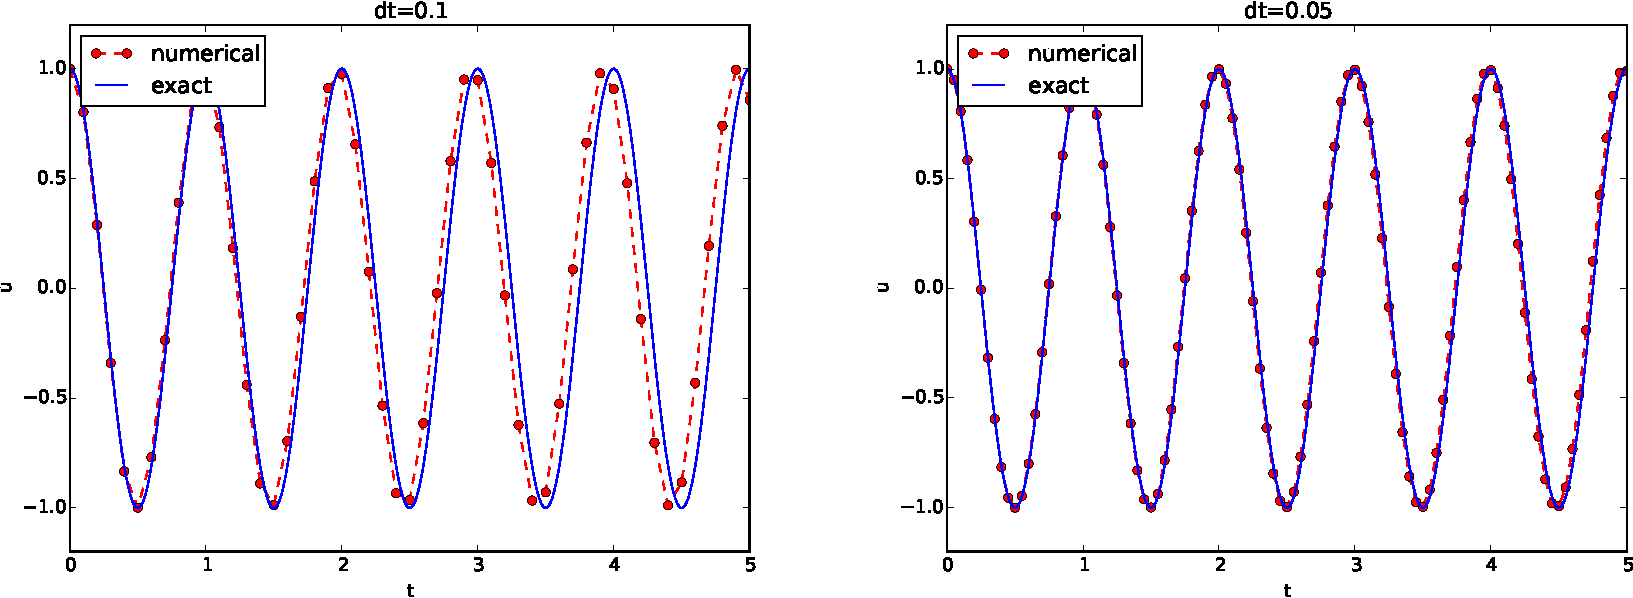
\includegraphics[width=1.0\linewidth]{fig-vib/vib_freq_err1.pdf}}
  \caption{
  Effect of halving the time step. \label{vib:ode1:2dt}
  }
\end{figure}
%\clearpage % flush figures vib:ode1:2dt


\subsection{Using a moving plot window}

In vibration problems it is often of interest to investigate the system's
behavior over long time intervals. Errors in the angular frequency accumulate
and become more visible as time grows. We can investigate long
time series by introducing a moving plot window that can move along with
the $p$ most recently computed periods of the solution. The
\href{{https://github.com/hplgit/scitools}}{SciTools} package contains
a convenient tool for this: \texttt{MovingPlotWindow}. Typing
\texttt{pydoc scitools.MovingPlotWindow} shows a demo and a description of its use.
The function below utilizes the moving plot window and is in fact
called by the \texttt{main} function the \Verb!vib_undamped! module
if the number of periods in the simulation exceeds 10.

\begin{cod}{cbg_blue1}\begin{Verbatim}[numbers=none,fontsize=\fontsize{9pt}{9pt},baselinestretch=0.95,xleftmargin=2mm]
def visualize_front(u, t, I, w, savefig=False, skip_frames=1):
    """
    Visualize u and the exact solution vs t, using a
    moving plot window and continuous drawing of the
    curves as they evolve in time.
    Makes it easy to plot very long time series.
    Plots are saved to files if savefig is True.
    Only each skip_frames-th plot is saved (e.g., if
    skip_frame=10, only each 10th plot is saved to file;
    this is convenient if plot files corresponding to
    different time steps are to be compared).
    """
    import scitools.std as st
    from scitools.MovingPlotWindow import MovingPlotWindow
    from math import pi

    # Remove all old plot files tmp_*.png
    import glob, os
    for filename in glob.glob('tmp_*.png'):
        os.remove(filename)

    P = 2*pi/w  # one period
    umin = 1.2*u.min();  umax = -umin
    dt = t[1] - t[0]
    plot_manager = MovingPlotWindow(
        window_width=8*P,
        dt=dt,
        yaxis=[umin, umax],
        mode='continuous drawing')
    frame_counter = 0
    for n in range(1,len(u)):
        if plot_manager.plot(n):
            s = plot_manager.first_index_in_plot
            st.plot(t[s:n+1], u[s:n+1], 'r-1',
                    t[s:n+1], I*cos(w*t)[s:n+1], 'b-1',
                    title='t=%6.3f' % t[n],
                    axis=plot_manager.axis(),
                    show=not savefig) # drop window if savefig
            if savefig and n % skip_frames == 0:
                filename = 'tmp_%04d.png' % frame_counter
                st.savefig(filename)
                print 'making plot file', filename, 'at t=%g' % t[n]
                frame_counter += 1
        plot_manager.update(n)
\end{Verbatim}
\end{cod}
\noindent

We run the scaled problem (the default values for the command-line arguments
\texttt{--I} and \texttt{--w} correspond to the scaled problem) for 40 periods with 20
time steps per period:

\begin{Verbatim}[frame=lines,label=\fbox{{\tiny Terminal}},framesep=2.5mm,framerule=0.7pt,fontsize=\fontsize{9pt}{9pt}]
Terminal> python vib_undamped.py --dt 0.05 --num_periods 40
\end{Verbatim}
The moving plot window is invoked, and we can follow the numerical and exact
solutions as time progresses. From this demo we see that
the angular frequency error is small in the beginning, but it becomes more
prominent with time. A new run with $\Delta t=0.1$ (i.e., only 10 time steps per period)
clearly shows that the phase errors become significant even earlier
in the time series, deteriorating the solution further.

\subsection{Making animations}
\label{vib:ode1:anim}

\index{making movies}
\index{animation}
\index{WebM (video format)}
\index{Ogg (video format)}
\index{MP4 (video format)}
\index{Flash (video format)}
\index{video formats}

\paragraph{Producing standard video formats.}
The \Verb!visualize_front! function stores all the plots in
files whose names are numbered:
\Verb!tmp_0000.png!, \Verb!tmp_0001.png!, \Verb!tmp_0002.png!,
and so on. From these files we may make a movie. The Flash
format is popular,

\begin{Verbatim}[frame=lines,label=\fbox{{\tiny Terminal}},framesep=2.5mm,framerule=0.7pt,fontsize=\fontsize{9pt}{9pt}]
Terminal> ffmpeg -r 12 -i tmp_%04d.png -c:v flv movie.flv
\end{Verbatim}
The \texttt{ffmpeg} program can be replaced by the \texttt{avconv} program in
the above command if desired (but at the time of this writing it seems
to be more momentum in the \texttt{ffmpeg} project).
The \texttt{-r} option should come first and
describes the number of frames per second in the movie. The
\texttt{-i} option describes the name of the plot files.
Other formats can be generated by changing the video codec
and equipping the video file with the right extension:


\begin{center}
\begin{tabular}{ll}
\hline
\multicolumn{1}{c}{ Format } & \multicolumn{1}{c}{ Codec and filename } \\
\hline
Flash  & \texttt{-c:v flv movie.flv}       \\
MP4    & \texttt{-c:v libx264 movie.mp4}   \\
WebM   & \texttt{-c:v libvpx movie.webm}   \\
Ogg    & \texttt{-c:v libtheora movie.ogg} \\
\hline
\end{tabular}
\end{center}

\noindent
\index{HTML5 video tag}

The video file can be played by some video player like \texttt{vlc}, \texttt{mplayer},
\texttt{gxine}, or \texttt{totem}, e.g.,

\begin{Verbatim}[frame=lines,label=\fbox{{\tiny Terminal}},framesep=2.5mm,framerule=0.7pt,fontsize=\fontsize{9pt}{9pt}]
Terminal> vlc movie.webm
\end{Verbatim}
A web page can also be used to play the movie. Today's standard is
to use the HTML5 \texttt{video} tag:

\begin{cod}{cbg_blue1}\begin{Verbatim}[numbers=none,fontsize=\fontsize{9pt}{9pt},baselinestretch=0.95,xleftmargin=2mm]
<video autoplay loop controls
       width='640' height='365' preload='none'>
<source src='movie.webm'  type='video/webm; codecs="vp8, vorbis"'>
</video>
\end{Verbatim}
\end{cod}
\noindent
Modern browsers do not support all of the video formats.
MP4 is needed to successfully play the videos on Apple devices
that use the Safari browser.
WebM is the preferred format for Chrome, Opera, Firefox, and Internet
Explorer v9+. Flash was a popular format, but older browsers that
required Flash can play MP4. All browsers that work with Ogg can also
work with WebM. This means that to have a video work in all browsers,
the video should be available in the MP4 and WebM formats.
The proper HTML code reads

\begin{cod}{cbg_blue1}\begin{Verbatim}[numbers=none,fontsize=\fontsize{9pt}{9pt},baselinestretch=0.95,xleftmargin=2mm]
<video autoplay loop controls
       width='640' height='365' preload='none'>
<source src='movie.mp4'   type='video/mp4;
 codecs="avc1.42E01E, mp4a.40.2"'>
<source src='movie.webm'  type='video/webm;
 codecs="vp8, vorbis"'>
</video>
\end{Verbatim}
\end{cod}
\noindent
The MP4 format should appear first to ensure that Apple devices will
load the video correctly.


\begin{warning_mdfboxadmon}[Caution: number the plot files correctly.]
To ensure that the individual plot frames are shown in correct order,
it is important to number the files with zero-padded numbers
(0000, 0001, 0002, etc.). The printf format \Verb!%04d! specifies an
integer in a field of width 4, padded with zeros from the left.
A simple Unix wildcard file specification like \Verb!tmp_*.png!
will then list the frames in the right order. If the numbers in the
filenames were not zero-padded, the frame \Verb!tmp_11.png! would appear
before \Verb!tmp_2.png! in the movie.
\end{warning_mdfboxadmon}



\paragraph{Paying PNG files in a web browser.}
\index{scitools movie@{\rm\texttt{scitools movie}} command}

The \texttt{scitools movie} command can create a movie player for a set
of PNG files such that a web browser can be used to watch the movie.
This interface has the advantage that the speed of the movie can
easily be controlled, a feature that scientists often appreciate.
The command for creating an HTML with a player for a set of
PNG files \Verb!tmp_*.png! goes like

\begin{Verbatim}[frame=lines,label=\fbox{{\tiny Terminal}},framesep=2.5mm,framerule=0.7pt,fontsize=\fontsize{9pt}{9pt}]
Terminal> scitools movie output_file=vib.html fps=4 tmp_*.png
\end{Verbatim}
The \texttt{fps} argument controls the speed of the movie (``frames per second'').

To watch the movie, load the video file \texttt{vib.html} into some browser, e.g.,
\begin{Verbatim}[frame=lines,label=\fbox{{\tiny Terminal}},framesep=2.5mm,framerule=0.7pt,fontsize=\fontsize{9pt}{9pt}]
Terminal> google-chrome vib.html  # invoke web page
\end{Verbatim}
Clicking on \texttt{Start movie} to see the result. Moving this movie to
some other place requires moving \texttt{vib.html} \emph{and all the PNG files}
\Verb!tmp_*.png!:
\begin{Verbatim}[frame=lines,label=\fbox{{\tiny Terminal}},framesep=2.5mm,framerule=0.7pt,fontsize=\fontsize{9pt}{9pt}]
Terminal> mkdir vib_dt0.1
Terminal> mv tmp_*.png vib_dt0.1
Terminal> mv vib.html vib_dt0.1/index.html
\end{Verbatim}

\paragraph{Making animated GIF files.}
The \texttt{convert} program from the ImageMagick software suite can be
used to produce animated GIF files from a set of PNG files:

\begin{Verbatim}[frame=lines,label=\fbox{{\tiny Terminal}},framesep=2.5mm,framerule=0.7pt,fontsize=\fontsize{9pt}{9pt}]
Terminal> convert -delay 25 tmp_vib*.png tmp_vib.gif
\end{Verbatim}
The \texttt{-delay} option needs an argument of the delay between each frame,
measured in 1/100 s, so 4 frames/s here gives 25/100 s delay.
Note, however, that in this particular example
with $\Delta t=0.05$ and 40 periods,
making an animated GIF file out of
the large number of PNG files is a very heavy process and not
considered feasible. Animated GIFs are best suited for animations with
not so many frames and where you want to see each frame and play them
slowly.

\shortinlinecomment{hpl 5}{ Combine two simulations side by side! }{ Combine two simulations side }

\subsection{Using Bokeh to compare graphs}

Instead of a moving plot frame, one can use tools that allows panning
by the mouse. For example, we can show four periods of a signal in
a plot and then scroll with the mouse through the rest of the
simulation. The \href{{http://bokeh.pydata.org/en/latest/docs/quickstart.html}}{Bokeh} plotting library offers such tools, but the plot must be displayed in
a web browser. The documentation of Bokeh is excellent, so here we just
show how the library can be used to compare a set of $u$ curves corresponding
to long time simulations.

Imagine we have performed experiments for a set of $\Delta t$ values.
We want each curve, together with the exact solution, to appear in
a plot, and then arrange all plots in a grid-like fashion:



% inline figure
\centerline{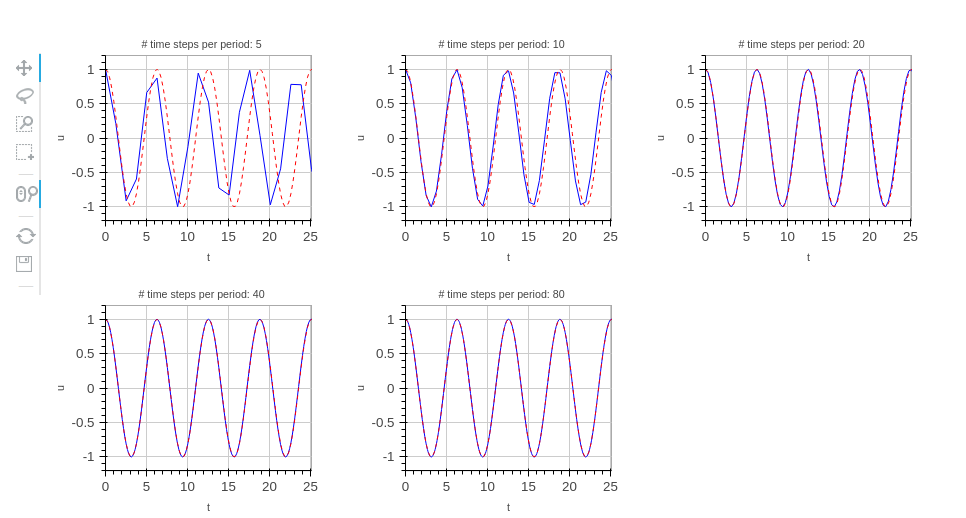
\includegraphics[width=1.0\linewidth]{fig-vib/bokeh_gridplot1.png}}



Furthermore, we want the axis to couple such that if we move into
the future in one plot, all the other plots follows (note the
displaced $t$ axes!):



% inline figure
\centerline{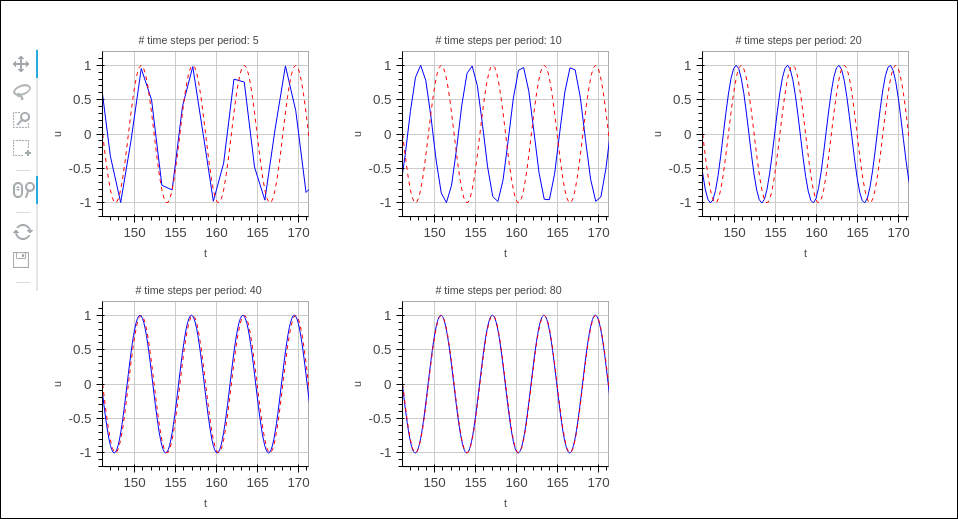
\includegraphics[width=1.0\linewidth]{fig-vib/bokeh_gridplot2.png}}




A function for creating a Bokeh plot, given a list of \texttt{u} arrays
and corresponding \texttt{t} arrays, from different simulations, described
compactly in a list of strings \texttt{legends}, takes the following form:

\begin{cod}{cbg_blue1}\begin{Verbatim}[numbers=none,fontsize=\fontsize{9pt}{9pt},baselinestretch=0.95,xleftmargin=2mm]
def bokeh_plot(u, t, legends, I, w, t_range, filename):
    """
    Make plots for u vs t using the Bokeh library.
    u and t are lists (several experiments can be compared).
    legens contain legend strings for the various u,t pairs.
    """
    if not isinstance(u, (list,tuple)):
        u = [u]  # wrap in list
    if not isinstance(t, (list,tuple)):
        t = [t]  # wrap in list
    if not isinstance(legends, (list,tuple)):
        legends = [legends]  # wrap in list

    import bokeh.plotting as plt
    plt.output_file(filename, mode='cdn', title='Comparison')
    # Assume that all t arrays have the same range
    t_fine = np.linspace(0, t[0][-1], 1001)  # fine mesh for u_e
    tools = 'pan,wheel_zoom,box_zoom,reset,'\ 
            'save,box_select,lasso_select'
    u_range = [-1.2*I, 1.2*I]
    font_size = '8pt'
    p = []  # list of plot objects
    # Make the first figure
    p_ = plt.figure(
        width=300, plot_height=250, title=legends[0],
        x_axis_label='t', y_axis_label='u',
        x_range=t_range, y_range=u_range, tools=tools,
        title_text_font_size=font_size)
    p_.xaxis.axis_label_text_font_size=font_size
    p_.yaxis.axis_label_text_font_size=font_size
    p_.line(t[0], u[0], line_color='blue')
    # Add exact solution
    u_e = u_exact(t_fine, I, w)
    p_.line(t_fine, u_e, line_color='red', line_dash='4 4')
    p.append(p_)
    # Make the rest of the figures and attach their axes to
    # the first figure's axes
    for i in range(1, len(t)):
        p_ = plt.figure(
            width=300, plot_height=250, title=legends[i],
            x_axis_label='t', y_axis_label='u',
            x_range=p[0].x_range, y_range=p[0].y_range, tools=tools,
            title_text_font_size=font_size)
        p_.xaxis.axis_label_text_font_size = font_size
        p_.yaxis.axis_label_text_font_size = font_size
        p_.line(t[i], u[i], line_color='blue')
        p_.line(t_fine, u_e, line_color='red', line_dash='4 4')
        p.append(p_)

    # Arrange all plots in a grid with 3 plots per row
    grid = [[]]
    for i, p_ in enumerate(p):
        grid[-1].append(p_)
        if (i+1) % 3 == 0:
            # New row
            grid.append([])
    plot = plt.gridplot(grid, toolbar_location='left')
    plt.save(plot)
    plt.show(plot)
\end{Verbatim}
\end{cod}
\noindent
A particular example using the \Verb!bokeh_plot! function appears below.

\begin{cod}{cbg_blue1}\begin{Verbatim}[numbers=none,fontsize=\fontsize{9pt}{9pt},baselinestretch=0.95,xleftmargin=2mm]
def demo_bokeh():
    """Solve a scaled ODE u'' + u = 0."""
    from math import pi
    w = 1.0        # Scaled problem (frequency)
    P = 2*np.pi/w  # Period
    num_steps_per_period = [5, 10, 20, 40, 80]
    T = 40*P       # Simulation time: 40 periods
    u = []         # List of numerical solutions
    t = []         # List of corresponding meshes
    legends = []
    for n in num_steps_per_period:
        dt = P/n
        u_, t_ = solver(I=1, w=w, dt=dt, T=T)
        u.append(u_)
        t.append(t_)
        legends.append('# time steps per period: %d' % n)
    bokeh_plot(u, t, legends, I=1, w=w, t_range=[0, 4*P],
               filename='tmp.html')
\end{Verbatim}
\end{cod}
\noindent

\subsection{Using a line-by-line ascii plotter}

Plotting functions vertically, line by line, in the terminal window
using ascii characters only is a simple, fast, and convenient
visualization technique for long time series. Note that the time
axis then is positive downwards on the screen.
The tool
\texttt{scitools.avplotter.Plotter} makes it easy to create such plots:

\begin{cod}{cbg_blue1}\begin{Verbatim}[numbers=none,fontsize=\fontsize{9pt}{9pt},baselinestretch=0.95,xleftmargin=2mm]
def visualize_front_ascii(u, t, I, w, fps=10):
    """
    Plot u and the exact solution vs t line by line in a
    terminal window (only using ascii characters).
    Makes it easy to plot very long time series.
    """
    from scitools.avplotter import Plotter
    import time
    from math import pi
    P = 2*pi/w
    umin = 1.2*u.min();  umax = -umin

    p = Plotter(ymin=umin, ymax=umax, width=60, symbols='+o')
    for n in range(len(u)):
        print p.plot(t[n], u[n], I*cos(w*t[n])), \ 
              '%.1f' % (t[n]/P)
        time.sleep(1/float(fps))
\end{Verbatim}
\end{cod}
\noindent
The call \texttt{p.plot} returns a line of text, with the $t$ axis marked and
a symbol \texttt{+} for the first function (\texttt{u}) and \texttt{o} for the second
function (the exact solution). Here we append to this text
a time counter reflecting how many periods the current time point
corresponds to. A typical output ($\omega =2\pi$, $\Delta t=0.05$)
looks like this:

\begin{cod}{cbg_blue1}\begin{Verbatim}[numbers=none,fontsize=\fontsize{9pt}{9pt},baselinestretch=0.95,xleftmargin=2mm]
                              |                       o+      14.0
                              |                      + o      14.0
                              |                  +    o       14.1
                              |             +     o           14.1
                              |     +        o                14.2
                             +|       o                       14.2
                     +        |                               14.2
              +       o       |                               14.3
         +     o              |                               14.4
      +   o                   |                               14.4
     +o                       |                               14.5
     o +                      |                               14.5
      o    +                  |                               14.6
          o      +            |                               14.6
               o        +     |                               14.7
                      o       | +                             14.7
                              |        +                      14.8
                              |       o       +               14.8
                              |              o     +          14.9
                              |                   o   +       14.9
                              |                       o+      15.0
\end{Verbatim}
\end{cod}
\noindent


\subsection{Empirical analysis of the solution}
\label{vib:ode1:empirical}

For oscillating functions like those in Figure~\ref{vib:ode1:2dt} we may
compute the amplitude and frequency (or period) empirically.
That is, we run through the discrete solution points $(t_n, u_n)$ and
find all maxima and minima points. The distance between two consecutive
maxima (or minima) points can be used as estimate of the local period,
while half the difference between the $u$ value at a maximum and a nearby
minimum gives an estimate of the local amplitude.

The local maxima are the points where
\begin{equation}
u^{n-1} < u^n > u^{n+1},\quad n=1,\ldots,N_t-1,
\end{equation}
and the local minima are recognized by
\begin{equation}
u^{n-1} > u^n < u^{n+1},\quad n=1,\ldots,N_t-1
\tp
\end{equation}
In computer code this becomes

\begin{cod}{cbg_blue1}\begin{Verbatim}[numbers=none,fontsize=\fontsize{9pt}{9pt},baselinestretch=0.95,xleftmargin=2mm]
def minmax(t, u):
    minima = []; maxima = []
    for n in range(1, len(u)-1, 1):
        if u[n-1] > u[n] < u[n+1]:
            minima.append((t[n], u[n]))
        if u[n-1] < u[n] > u[n+1]:
            maxima.append((t[n], u[n]))
    return minima, maxima
\end{Verbatim}
\end{cod}
\noindent
Note that the two returned objects are lists of tuples.

Let $(t_i, e_i)$, $i=0,\ldots,M-1$, be the sequence of all
the $M$ maxima points, where $t_i$
is the time value and $e_i$ the corresponding $u$ value.
The local period can be defined as $p_i=t_{i+1}-t_i$.
With Python syntax this reads

\begin{cod}{cbg_blue1}\begin{Verbatim}[numbers=none,fontsize=\fontsize{9pt}{9pt},baselinestretch=0.95,xleftmargin=2mm]
def periods(maxima):
    p = [extrema[n][0] - maxima[n-1][0]
         for n in range(1, len(maxima))]
    return np.array(p)
\end{Verbatim}
\end{cod}
\noindent
The list \texttt{p} created by a list comprehension is converted to an array
since we probably want to compute with it, e.g., find the corresponding
frequencies \texttt{2*pi/p}.

Having the minima and the maxima, the local amplitude can be
calculated as the difference between two neighboring minimum and
maximum points:

\begin{cod}{cbg_blue1}\begin{Verbatim}[numbers=none,fontsize=\fontsize{9pt}{9pt},baselinestretch=0.95,xleftmargin=2mm]
def amplitudes(minima, maxima):
    a = [(abs(maxima[n][1] - minima[n][1]))/2.0
         for n in range(min(len(minima),len(maxima)))]
    return np.array(a)
\end{Verbatim}
\end{cod}
\noindent
The code segments are found in the file \href{{http://tinyurl.com/nm5587k/vib/vib_empirical_analysis.py}}{\nolinkurl{vib_empirical_analysis.py}}.

Since \texttt{a[i]} and \texttt{p[i]} correspond to
the $i$-th amplitude estimate and the $i$-th period estimate, respectively,
it is most convenient to visualize the \texttt{a} and \texttt{p} values with the
index \texttt{i} on the horizontal axis.
(There is no unique time point associated with either of these estimate
since values at two different time points were used in the
computations.)

In the analysis of very long time series, it is advantageous to
compute and plot \texttt{p} and \texttt{a} instead of $u$ to get an impression of
the development of the oscillations. Let us do this for the scaled
problem and $\Delta t=0.1, 0.05, 0.01$.
A ready-made function

\begin{cod}{cbg_blue1}\begin{Verbatim}[numbers=none,fontsize=\fontsize{9pt}{9pt},baselinestretch=0.95,xleftmargin=2mm]
plot_empirical_freq_and_amplitude(u, t, I, w)
\end{Verbatim}
\end{cod}
\noindent
computes the empirical amplitudes and periods, and creates a plot
where the amplitudes and angular frequencies
are visualized together with the exact amplitude \texttt{I}
and the exact angular frequency \texttt{w}. We can make a little program
for creating the plot:

\begin{pro}{cbg_blue1}{bar_blue1}\begin{Verbatim}[numbers=none,fontsize=\fontsize{9pt}{9pt},baselinestretch=0.95,xleftmargin=2mm]
from vib_undamped import solver, plot_empirical_freq_and_amplitude
from math import pi
dt_values = [0.1, 0.05, 0.01]
u_cases = []
t_cases = []
for dt in dt_values:
    # Simulate scaled problem for 40 periods
    u, t = solver(I=1, w=2*pi, dt=dt, T=40)
    u_cases.append(u)
    t_cases.append(t)
plot_empirical_freq_and_amplitude(u_cases, t_cases, I=1, w=2*pi)
\end{Verbatim}
\end{pro}
\noindent
Figure~\ref{vib:ode1:fig:freq_ampl} shows the result: we clearly see that
lowering $\Delta t$ improves the angular frequency significantly, while the
amplitude seems to be more accurate.
The lines with
$\Delta t=0.01$, corresponding to 100 steps per period, can hardly be
distinguished from the exact values. The next section shows how we
can get mathematical insight into why amplitudes are good and frequencies
are more inaccurate.


\begin{figure}[!ht]  % vib:ode1:fig:freq_ampl
  \centerline{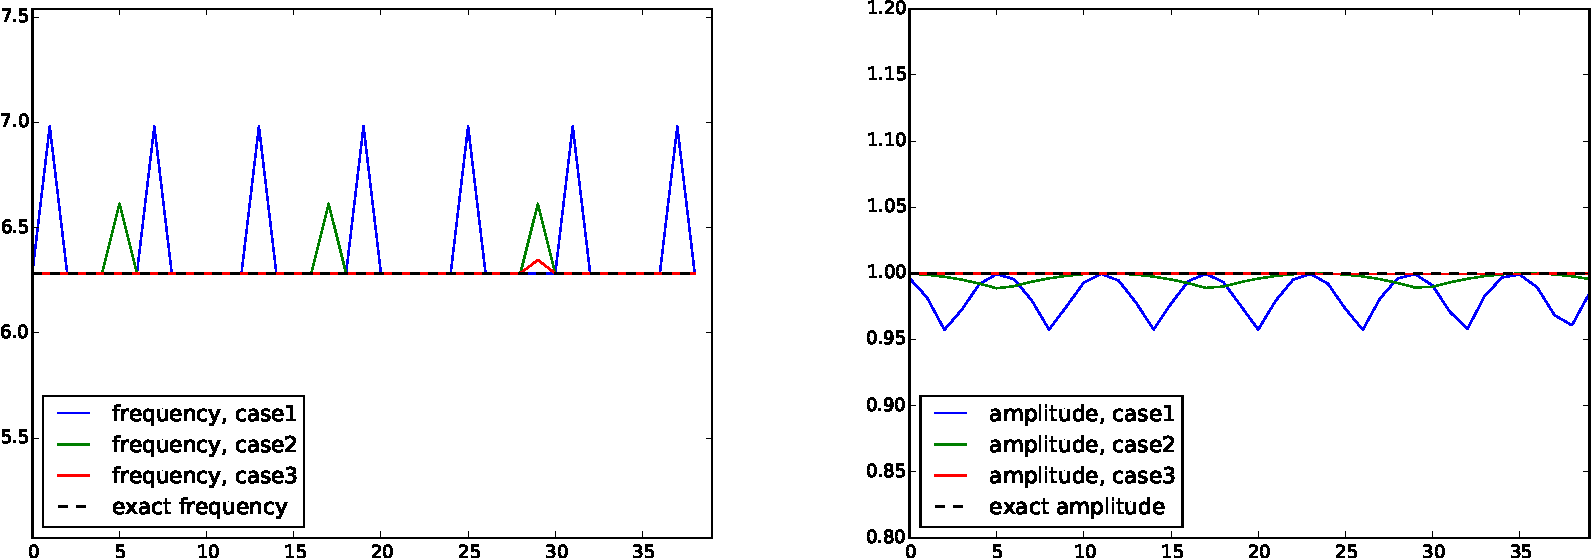
\includegraphics[width=1.0\linewidth]{fig-vib/empirical_ampl_freq.pdf}}
  \caption{
  Empirical amplitude and angular frequency for three cases of time steps. \label{vib:ode1:fig:freq_ampl}
  }
\end{figure}
%\clearpage % flush figures vib:ode1:fig:freq_ampl


% Use it for very long time integration of CN! And of RK4!

\section{Analysis of the numerical scheme}
\label{vib:ode1:analysis}

\subsection{Deriving a solution of the numerical scheme}

After having seen the phase error grow with time in the previous
section, we shall now quantify this error through mathematical
analysis.  The key tool in the analysis will be to establish an exact
solution of the discrete equations.  The difference equation
(\ref{vib:ode1:step4}) has constant coefficients and is
homogeneous. Such equations are known to have solutions on the form
$u^n=CA^n$, where $A$ is some number
to be determined from the difference equation and $C$ is found as the
initial condition ($C=I$).  Recall that $n$ in $u^n$ is a
superscript labeling the time level, while $n$ in $A^n$ is an
exponent.

With oscillating functions as solutions, the algebra will
be considerably simplified if we seek an $A$ on the form

\[ A=e^{i\tilde\omega \Delta t},\]
and solve for the numerical frequency $\tilde\omega$ rather than
$A$. Note that $i=\sqrt{-1}$ is the imaginary unit. (Using a
complex exponential function gives simpler arithmetics than working
with a sine or cosine function.)
We have

\[
A^n = e^{i\tilde\omega \Delta t\, n}=e^{i\tilde\omega t} =
\cos (\tilde\omega t) + i\sin(\tilde \omega t)
\tp
\]
The physically relevant numerical solution can
be taken as the real part of this complex expression.

The calculations go as

\begin{align*}
[D_tD_t u]^n &= \frac{u^{n+1} - 2u^n + u^{n-1}}{\Delta t^2}\\ 
&= I\frac{A^{n+1} - 2A^n + A^{n-1}}{\Delta t^2}\\ 
&= \frac{I}{\Delta t^{2}}(e^{i\tilde\omega(t+\Delta t)} - 2e^{i\tilde\omega t} + e^{i\tilde\omega(t-\Delta t)})\\ 
&= Ie^{i\tilde\omega t}\frac{1}{\Delta t^2}\left(e^{i\tilde\omega\Delta t} + e^{i\tilde\omega(-\Delta t)} - 2\right)\\ 
&= Ie^{i\tilde\omega t}\frac{2}{\Delta t^2}\left(\cosh(i\tilde\omega\Delta t) -1 \right)\\ 
&= Ie^{i\tilde\omega t}\frac{2}{\Delta t^2}\left(\cos(\tilde\omega\Delta t) -1 \right)\\ 
&= -Ie^{i\tilde\omega t}\frac{4}{\Delta t^2}\sin^2(\frac{\tilde\omega\Delta t}{2})
\end{align*}
The last line follows from the relation
$\cos x - 1 = -2\sin^2(x/2)$ (try \texttt{cos(x)-1} in
\href{{http://www.wolframalpha.com}}{wolframalpha.com} to see the formula).

The scheme (\ref{vib:ode1:step4})
with $u^n=Ie^{i\omega\tilde\Delta t\, n}$ inserted now gives

\begin{equation}
-Ie^{i\tilde\omega t}\frac{4}{\Delta t^2}\sin^2(\frac{\tilde\omega\Delta t}{2})
+ \omega^2 Ie^{i\tilde\omega t} = 0,
\end{equation}
which after dividing by $Ie^{i\tilde\omega t}$ results in
\begin{equation}
\frac{4}{\Delta t^2}\sin^2(\frac{\tilde\omega\Delta t}{2}) = \omega^2
\tp
\end{equation}
The first step in solving for the unknown $\tilde\omega$ is
\[ \sin^2(\frac{\tilde\omega\Delta t}{2}) = \left(\frac{\omega\Delta t}{2}\right)^2
\tp
\]
Then, taking the square root, applying the inverse sine function, and
multiplying by $2/\Delta t$, results in
\begin{equation}
\tilde\omega = \pm \frac{2}{\Delta t}\sin^{-1}\left(\frac{\omega\Delta t}{2}\right)
\tp
\label{vib:ode1:tildeomega}
\end{equation}

The first observation of (\ref{vib:ode1:tildeomega}) tells that
there is a phase error since the numerical frequency $\tilde\omega$
never equals the exact frequency $\omega$. But how good is
the approximation (\ref{vib:ode1:tildeomega})? That is, what
is the error $\omega - \tilde\omega$ or $\tilde\omega/\omega$?
Taylor series expansion
for small $\Delta t$ may give an expression that is easier to understand
than the complicated function in (\ref{vib:ode1:tildeomega}):

\begin{cod}{cbg_blue1}\begin{Verbatim}[numbers=none,fontsize=\fontsize{9pt}{9pt},baselinestretch=0.95,xleftmargin=2mm]
>>> from sympy import *
>>> dt, w = symbols('dt w')
>>> w_tilde_e = 2/dt*asin(w*dt/2)
>>> w_tilde_series = w_tilde_e.series(dt, 0, 4)
>>> print w_tilde_series
w + dt**2*w**3/24 + O(dt**4)
\end{Verbatim}
\end{cod}
\noindent
This means that

% See vib_symbolic.py for computations with sympy
\begin{equation}
\tilde\omega = \omega\left( 1 + \frac{1}{24}\omega^2\Delta t^2\right)
+ \Oof{\Delta t^4}
\tp
\label{vib:ode1:tildeomega:series}
\end{equation}
The error in the numerical frequency is of second-order in
$\Delta t$, and the error vanishes as $\Delta t\rightarrow 0$.
We see that $\tilde\omega > \omega$ since the term $\omega^3\Delta t^2/24 >0$
and this is by far the biggest term in the series expansion for small
$\omega\Delta t$. A numerical frequency that is too large gives an oscillating
curve that oscillates too fast and therefore ``lags behind'' the exact
oscillations, a feature that can be seen in the left plot in Figure~\ref{vib:ode1:2dt}.

Figure~\ref{vib:ode1:tildeomega:plot} plots the discrete frequency
(\ref{vib:ode1:tildeomega})
and its approximation (\ref{vib:ode1:tildeomega:series}) for $\omega =1$ (based
on the program \href{{http://tinyurl.com/nm5587k/vib/vib_plot_freq.py}}{\nolinkurl{vib_plot_freq.py}}).
Although $\tilde\omega$ is a function of $\Delta t$ in
(\ref{vib:ode1:tildeomega:series}),
it is misleading to think of $\Delta t$ as the important
discretization parameter. It is the product $\omega\Delta t$ that is
the key discretization parameter. This quantity reflects the
\emph{number of time steps per period} of the oscillations.
To see this, we set $P=N_P\Delta t$, where $P$ is the length of
a period, and $N_P$ is the number of time steps during a period.
Since $P$ and $\omega$ are related by $P=2\pi/\omega$,
we get that $\omega\Delta t = 2\pi/N_P$, which shows that
$\omega\Delta t$ is directly related to $N_P$.

The plot shows
that at least $N_P\sim 25-30$ points per period are necessary for reasonable
accuracy, but this depends on the length of the simulation ($T$) as
the total phase error due to the frequency error grows linearly with time
(see Exercise~\ref{vib:exer:phase:err:growth}).


\begin{figure}[!ht]  % vib:ode1:tildeomega:plot
  \centerline{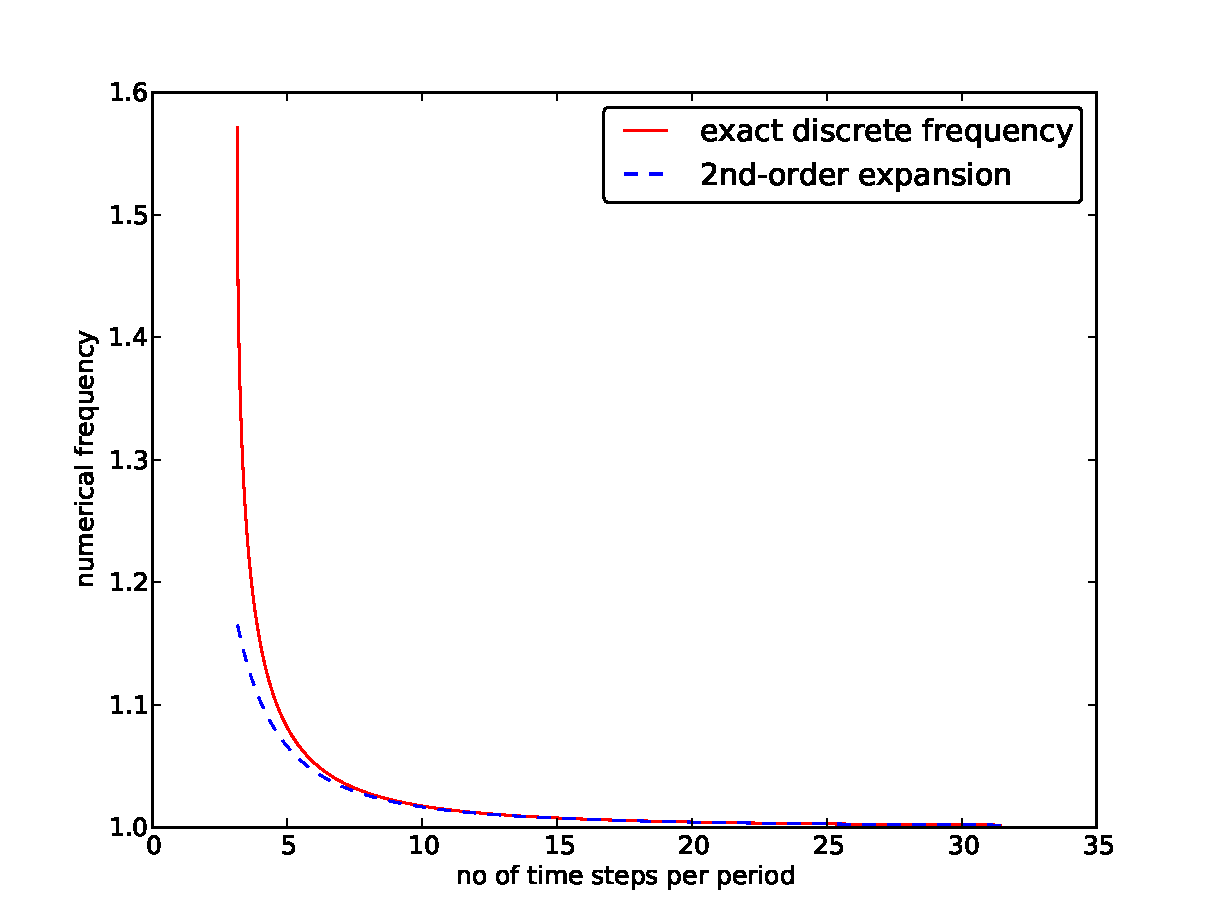
\includegraphics[width=0.9\linewidth]{fig-vib/discrete_freq.pdf}}
  \caption{
  Exact discrete frequency and its second-order series expansion. \label{vib:ode1:tildeomega:plot}
  }
\end{figure}
%\clearpage % flush figures vib:ode1:tildeomega:plot



\subsection{Exact discrete solution}
\label{vib:ode1:analysis:sol}

Perhaps more important than the $\tilde\omega = \omega + {\cal O}(\Delta t^2)$
result found above is the fact that we have an exact discrete solution of
the problem:

\begin{equation}
u^n = I\cos\left(\tilde\omega n\Delta t\right),\quad
\tilde\omega = \frac{2}{\Delta t}\sin^{-1}\left(\frac{\omega\Delta t}{2}\right)
\tp
\label{vib:ode1:un:exact}
\end{equation}
We can then compute the error mesh function

\begin{equation}
e^n = \uex(t_n) - u^n =
I\cos\left(\omega n\Delta t\right) - I\cos\left(\tilde\omega n\Delta t\right)\tp
\label{vib:ode1:en}
\end{equation}
From the formula $\cos 2x - \cos 2y = -2\sin(x-y)\sin(x+y)$ we can
rewrite $e^n$ so the expression is easier to interpret:

\begin{equation}
e^n = -2I\sin\left(t\half\left( \omega - \tilde\omega\right)\right)
\sin\left(t\half\left( \omega + \tilde\omega\right)\right)\tp
\label{vib:ode1:en2}
\end{equation}

The error mesh function is ideal for verification purposes
and you are strongly encouraged to make a test based on (\ref{vib:ode1:un:exact})
by doing Exercise~\ref{vib:exer:discrete:omega}.


\subsection{Convergence}
\label{vib:ode1:analysis:conv}


We can use (\ref{vib:ode1:tildeomega:series}), (\ref{vib:ode1:en}), or
(\ref{vib:ode1:en2}) to show \emph{convergence} of the
numerical scheme, i.e., $e^n\rightarrow 0$ as $\Delta t\rightarrow 0$.
We have that

\[
\lim_{\Delta t\rightarrow 0}
\tilde\omega = \lim_{\Delta t\rightarrow 0}
\frac{2}{\Delta t}\sin^{-1}\left(\frac{\omega\Delta t}{2}\right)
= \omega,
\]
by L'Hopital's rule or simply asking \texttt{sympy} or
\href{{http://www.wolframalpha.com/input/?i=%282%2Fx%29*asin%28w*x%2F2%29+as+x-%3E0}}{WolframAlpha} about the limit:

\begin{cod}{cbg_blue1}\begin{Verbatim}[numbers=none,fontsize=\fontsize{9pt}{9pt},baselinestretch=0.95,xleftmargin=2mm]
>>> import sympy as sym
>>> dt, w = sym.symbols('x w')
>>> sym.limit((2/dt)*sym.asin(w*dt/2), dt, 0, dir='+')
w
\end{Verbatim}
\end{cod}
\noindent
Also (\ref{vib:ode1:tildeomega:series}) can be used to establish
this result that
$\tilde\omega\rightarrow\omega$. It then follows from the expression(s)
for $e^n$ that $e^n\rightarrow 0$.

\subsection{The global error}

\index{error!global}

To achieve more analytical insight into the nature of the global error,
we can Taylor expand the error mesh function (\ref{vib:ode1:en}).
Since $\tilde\omega$ in (\ref{vib:ode1:tildeomega})
contains $\Delta t$ in the denominator we use the series expansion
for $\tilde\omega$ inside the cosine function. A relevant \texttt{sympy}
session is

\begin{cod}{cbg_blue1}\begin{Verbatim}[numbers=none,fontsize=\fontsize{9pt}{9pt},baselinestretch=0.95,xleftmargin=2mm]
>>> from sympy import *
>>> dt, w, t = symbols('dt w t')
>>> w_tilde_e = 2/dt*asin(w*dt/2)
>>> w_tilde_series = w_tilde_e.series(dt, 0, 4)
>>> w_tilde_series
w + dt**2*w**3/24 + O(dt**4)
\end{Verbatim}
\end{cod}
\noindent
Series expansions in \texttt{sympy} have the inconvenient \texttt{O()} term that
prevents further calculations with the series. We can use the
\texttt{removeO()} command to get rid of the \texttt{O()} term:

\begin{cod}{cbg_blue1}\begin{Verbatim}[numbers=none,fontsize=\fontsize{9pt}{9pt},baselinestretch=0.95,xleftmargin=2mm]
>>> w_tilde_series = w_tilde_series.removeO()
>>> w_tilde_series
dt**2*w**3/24 + w
\end{Verbatim}
\end{cod}
\noindent
Using this \Verb!w_tilde_series! expression
for $\tilde w$ in (\ref{vib:ode1:en}),
dropping $I$ (which is a common factor), and performing a series
expansion of the error yields

\begin{cod}{cbg_blue1}\begin{Verbatim}[numbers=none,fontsize=\fontsize{9pt}{9pt},baselinestretch=0.95,xleftmargin=2mm]
>>> error = cos(w*t) - cos(w_tilde_series*t)
>>> error.series(dt, 0, 6)
dt**2*t*w**3*sin(t*w)/24 + dt**4*t**2*w**6*cos(t*w)/1152 + O(dt**6)
\end{Verbatim}
\end{cod}
\noindent
Since we are mainly interested in the leading-order term in
such expansions (the term with lowest power in $\Delta t$ and
goes most slowly to zero), we use the \Verb!.as_leading_term(dt)!
construction to pick out this term:

\begin{cod}{cbg_blue1}\begin{Verbatim}[numbers=none,fontsize=\fontsize{9pt}{9pt},baselinestretch=0.95,xleftmargin=2mm]
>>> error.series(dt, 0, 6).as_leading_term(dt)
dt**2*t*w**3*sin(t*w)/24
\end{Verbatim}
\end{cod}
\noindent

The last result
means that the leading order global (true) error at a point $t$
is proportional to $\omega^3t\Delta t^2$. Now, $t$ is related
to $\Delta t$ through $t=n\Delta t$. The factor
$\sin(\omega t)$ can at most be 1, so we use this value to
bound the leading-order expression to its maximum value

\[ e^n = \frac{1}{24}n\omega^3\Delta t^3\tp\]
This is the dominating term of the error \emph{at a point}.

We are interested in the accumulated global error, which can
be taken as the $\ell^2$ norm of $e^n$.
The norm is simply computed by summing contributions from all mesh
points:

\[ ||e^n||_{\ell^2}^2 = \Delta t\sum_{n=0}^{N_t} \frac{1}{24^2}n^2\omega^6\Delta t^6
=\frac{1}{24^2}\omega^6\Delta t^7 \sum_{n=0}^{N_t} n^2\tp\]
The sum $\sum_{n=0}^{N_t} n^2$ is approximately equal to
$\frac{1}{3}N_t^3$. Replacing $N_t$ by $T/\Delta t$ and taking
the square root gives the expression

\[ ||e^n||_{\ell^2} = \frac{1}{24}\sqrt{\frac{T^3}{3}}\omega^3\Delta t^2\tp\]
This is our expression for the global (or integrated) error.
The main result from this expression is that also the global error
is proportional to $\Delta t^2$.



\subsection{Stability}

Looking at (\ref{vib:ode1:un:exact}), it appears that the numerical
solution has constant and correct amplitude, but an error in the
angular frequency. A constant amplitude is not necessarily the case,
however! To see this, note that if only $\Delta t$ is large
enough, the magnitude of the argument to $\sin^{-1}$ in
(\ref{vib:ode1:tildeomega}) may be larger than 1, i.e.,
$\omega\Delta t/2 > 1$. In this case, $\sin^{-1}(\omega\Delta t/2)$
has a complex value and therefore $\tilde\omega$ becomes complex.
Type, for example, \texttt{asin(x)} in
\href{{http://www.wolframalpha.com}}{wolframalpha.com} to see basic properties of $\sin^{-1} (x)$).

A complex $\tilde\omega$ can be written $\tilde\omega = \tilde\omega_r +
i\tilde\omega_i$. Since $\sin^{-1}(x)$ has a \emph{negative} imaginary part for
$x>1$, $\tilde\omega_i < 0$, which means that
$e^{i\tilde\omega t}=e^{-\tilde\omega_i t}e^{i\tilde\omega_r t}$
will lead to exponential growth in time because
$e^{-\tilde\omega_i t}$ with $\tilde\omega_i <0$ has a positive
exponent.

\index{stability criterion}


\begin{notice_mdfboxadmon}[Stability criterion.]
We do not tolerate growth in the amplitude since such growth is not
present in the exact solution. Therefore, we
must impose a \emph{stability criterion}  that
the argument in the inverse sine function leads
to real and not complex values of $\tilde\omega$. The stability
criterion reads

\begin{equation}
\frac{\omega\Delta t}{2} \leq 1\quad\Rightarrow\quad
\Delta t \leq \frac{2}{\omega}
\tp
\end{equation}
\end{notice_mdfboxadmon}



With $\omega =2\pi$, $\Delta t > \pi^{-1} = 0.3183098861837907$ will give
growing solutions. Figure~\ref{vib:ode1:dt:unstable}
displays what happens when $\Delta t =0.3184$,
which is slightly above the critical value: $\Delta t =\pi^{-1} + 9.01\cdot
10^{-5}$.


\begin{figure}[!ht]  % vib:ode1:dt:unstable
  \centerline{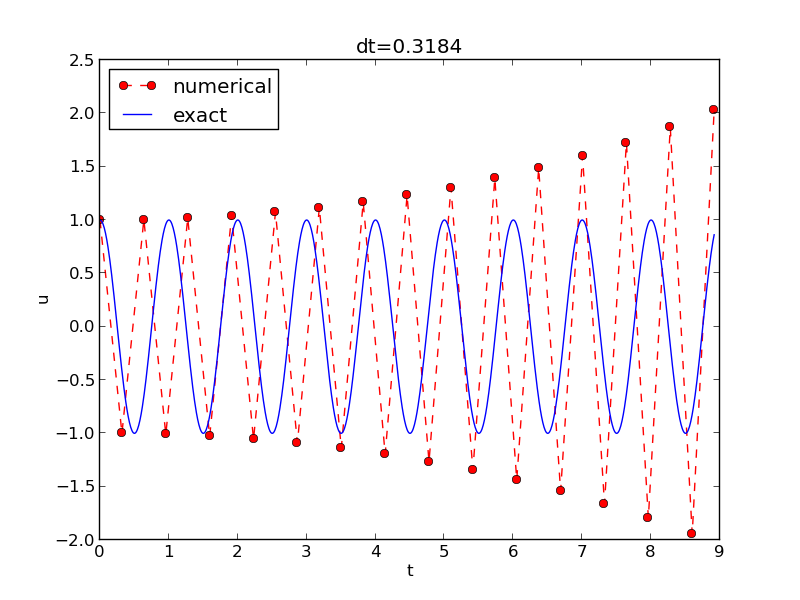
\includegraphics[width=0.9\linewidth]{fig-vib/vib_unstable.png}}
  \caption{
  Growing, unstable solution because of a time step slightly beyond the stability limit. \label{vib:ode1:dt:unstable}
  }
\end{figure}
%\clearpage % flush figures vib:ode1:dt:unstable


\subsection{About the accuracy at the stability limit}

An interesting question is whether the stability condition
$\Delta t < 2/\omega$ is unfortunate, or more precisely:
would it be meaningful to take larger time steps to speed up computations?
The answer is a clear no.~At the stability limit, we have that
$\sin^{-1}\omega\Delta t/2 = \sin^{-1} 1 = \pi/2$, and therefore
$\tilde\omega = \pi/\Delta t$. (Note that the approximate formula
(\ref{vib:ode1:tildeomega:series}) is very inaccurate for this
value of $\Delta t$ as it predicts $\tilde\omega = 2.34/pi$, which is
a 25 percent reduction.) The corresponding
period of the numerical solution
is $\tilde P=2\pi/\tilde\omega = 2\Delta t$, which means that there is
just one time step $\Delta t$ between a peak (maximum)
and a \href{{https://simple.wikipedia.org/wiki/Wave_(physics)}}{through}
(minimum) in the
numerical solution. This is the shortest possible wave that can be
represented in the mesh! In other words, it is not meaningful to
use a larger time step than the stability limit.

Also, the error in angular frequency
when $\Delta t = 2/\omega$ is severe: Figure~\ref{vib:ode1:dt:stablimit} shows a comparison of the numerical and
analytical solution with $\omega = 2\pi$ and
$\Delta t = 2/\omega = \pi^{-1}$. Already after one period, the
numerical solution has a through while the exact solution has a peak (!).
The error in frequency when $\Delta t$ is at the stability limit
becomes $\omega - \tilde\omega = \omega(1-\pi/2)\approx -0.57\omega$.
The corresponding error in the period is $P - \tilde P \approx 0.36P$.
The error after $m$ periods is then $0.36mP$. This error has reached
half a period when $m=1/(2\cdot 0.36)\approx 1.38$, which theoretically
confirms the observations in Figure~\ref{vib:ode1:dt:stablimit}
that the numerical solution is a through ahead of a peak already after
one and a half period. Consequently, $\Delta t$ should be chosen much
less than the stability limit to achieve meaningful numerical computations.


\begin{figure}[!ht]  % vib:ode1:dt:stablimit
  \centerline{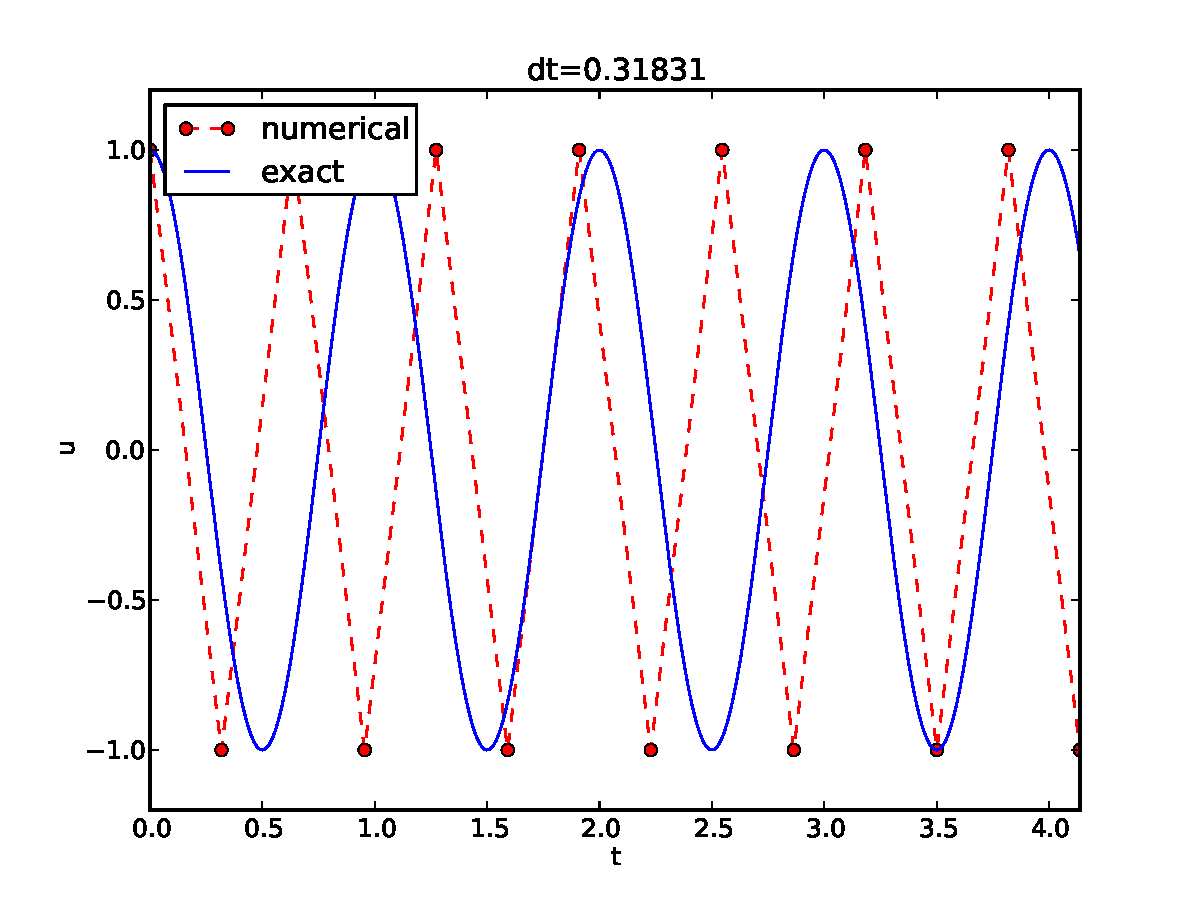
\includegraphics[width=0.9\linewidth]{fig-vib/vib_stability_limit.pdf}}
  \caption{
  Numerical solution with $\Delta t$ exactly at the stability limit. \label{vib:ode1:dt:stablimit}
  }
\end{figure}
%\clearpage % flush figures vib:ode1:dt:stablimit





\begin{summary_mdfboxadmon}[Summary.]
From the accuracy and stability
analysis we can draw three important conclusions:

\begin{enumerate}
\item The key parameter in the formulas is $p=\omega\Delta t$.
   The period of oscillations is $P=2\pi/\omega$, and the
   number of time steps per period is $N_P=P/\Delta t$.
   Therefore, $p=\omega\Delta t = 2\pi N_P$, showing that the
   critical parameter is the number of time steps per period.
   The smallest possible $N_P$ is 2, showing that $p\in (0,\pi]$.

\item Provided $p\leq 2$, the amplitude of the numerical solution is
   constant.

\item The ratio of the numerical angular frequency and the exact
   one is
   $\tilde\omega/\omega \approx 1 + \frac{1}{24}p^2$.
   The error $\frac{1}{24}p^2$ leads to wrongly displaced peaks of the numerical
   solution, and the error in peak location grows linearly with time
   (see Exercise~\ref{vib:exer:phase:err:growth}).
\end{enumerate}

\noindent
\end{summary_mdfboxadmon}






\section{Alternative schemes based on 1st-order equations}
\label{vib:model2x2}

A standard technique for solving second-order ODEs is
to rewrite them as a system of first-order ODEs and then choose a
solution strategy from the
vast collection of methods for first-order ODE systems.
Given the second-order ODE problem
\[ u^{\prime\prime} + \omega^2 u = 0,\quad u(0)=I,\ u^{\prime}(0)=0,\]
we introduce the auxiliary variable $v=u^{\prime}$ and express the ODE problem
in terms of first-order derivatives of $u$ and $v$:

\begin{align}
u^{\prime} &= v,
\label{vib:model2x2:ueq}\\ 
v' &= -\omega^2 u
\label{vib:model2x2:veq}
\tp
\end{align}
The initial conditions become $u(0)=I$ and $v(0)=0$.



\subsection{The Forward Euler scheme}

A Forward Euler approximation to our $2\times 2$ system of ODEs
(\ref{vib:model2x2:ueq})-(\ref{vib:model2x2:veq})
becomes

\begin{align}
\lbrack D_t^+ u = v\rbrack^n,
\lbrack D_t^+ v = -\omega^2 u\rbrack^n,
\end{align}
or written out,

\begin{align}
u^{n+1} &= u^n + \Delta t v^n,
\label{vib:undamped:FE1}\\ 
v^{n+1} &= v^n -\Delta t \omega^2 u^n
\label{vib:undamped:FE2}
\tp
\end{align}


Let us briefly compare this Forward Euler method with the
centered difference scheme for the second-order differential
equation. We have from (\ref{vib:undamped:FE1}) and
(\ref{vib:undamped:FE2}) applied at levels $n$ and $n-1$ that

\[ u^{n+1} = u^n + \Delta t v^n = u^n + \Delta t (v^{n-1} -\Delta t \omega^2 u^{n-1}\tp\]
Since from (\ref{vib:undamped:FE1})
\[ v^{n-1} = \frac{1}{\Delta t}(u^{n}-u^{n-1}),\]
it follows that

\[ u^{n+1} = 2u^n - u^{n-1} -\Delta t^2\omega^2 u^{n-1},\]
which is very close to the centered difference scheme, but
the last term is evaluated at $t_{n-1}$ instead of $t_n$.
Dividing by $\Delta t^2$, the left-hand side is an approximation to
$u^{\prime\prime}$ at $t_n$, while the right-hand side is sampled at $t_{n-1}$.
All terms should be sampled at the same mesh point, so using
$\omega^2 u^{n-1}$ instead of $\omega^2 u^n$ is an inconsistency
in the scheme. This inconsistency turns out to be rather
crucial for the accuracy of
the Forward Euler method applied to vibration problems.

\subsection{The Backward Euler scheme}

A Backward Euler approximation the ODE system is equally easy to
write up in the operator notation:

\begin{align}
\lbrack D_t^- u &= v\rbrack^{n+1},\\ 
\lbrack D_t^- v &= -\omega u\rbrack^{n+1} \tp
\end{align}
This becomes a coupled system for $u^{n+1}$ and $v^{n+1}$:

\begin{align}
u^{n+1} - \Delta t v^{n+1} &= u^{n},
\label{vib:undamped:BE1}\\ 
v^{n+1} + \Delta t \omega^2 u^{n+1} &= v^{n}
\label{vib:undamped:BE2}
\tp
\end{align}

We can compare (\ref{vib:undamped:BE1})-(\ref{vib:undamped:BE2}) with
the centered scheme (\ref{vib:ode1:step4})
for the second-order differential equation.
To this end, we eliminate $v^{n+1}$ in (\ref{vib:undamped:BE1})
using (\ref{vib:undamped:BE2}) solved with respect to $v^{n+1}$.
Thereafter, we eliminate $v^n$ using (\ref{vib:undamped:BE1})
solved with respect to $v^{n+1}$ and replacing $n+1$ by $n$.
The resulting equation involving only $u^{n+1}$, $u^n$, and $u^{n-1}$
can be ordered as

\[ \frac{u^{n+1}-2u^n+u^{n-1}}{\Delta t^2} = -\omega^2 u^{n+1},\]
which has almost the same form as the centered scheme for the
second-order differential equation, but the right-hand side is
evaluated at $u^{n+1}$ and not $u^n$. This inconsistent sampling
of terms has a dramatic effect on the numerical solution.

\subsection{The Crank-Nicolson scheme}

The Crank-Nicolson scheme takes this form in the operator notation:

\begin{align}
\lbrack D_t u &= \overline{v}^t\rbrack^{n+\half},\\ 
\lbrack D_t v &= -\omega \overline{u}^t\rbrack^{n+\half}
\tp
\end{align}
Writing the equations out shows that this is also a coupled system:

\begin{align}
u^{n+1} - \half\Delta t v^{n+1} &= u^{n} + \half\Delta t v^{n},\\ 
v^{n+1} + \half\Delta t \omega^2 u^{n+1} &= v^{n}
- \half\Delta t \omega^2 u^{n}
\tp
\end{align}

To see the nature of this approximation, and that it is actually
very promising, we write the equations as follows

\begin{align}
u^{n+1} - u^n &= \frac{1}{2}\Delta t(v^{n+1} + v^n),
\label{vib:undamped:CN3a}\\ 
v^{n+1}  &= v^n -\frac{1}{2}\Delta t(u^{n+1} + u^n),
\label{vib:undamped:CN4a}
\end{align}
and add the latter at the previous time level as well:

\begin{equation}
v^{n}  = v^{n-1} -\frac{1}{2}\Delta t(u^{n} + u^{n-1})
\label{vib:undamped:CN4b1}
\end{equation}
We can also rewrite (\ref{vib:undamped:CN3a}) at the previous time level
as

\begin{equation}
v^{n+1} + v^n = \frac{2}{\Delta t}(u^{n+1} - u^n)\tp
\label{vib:undamped:CN4b}
\end{equation}
Inserting (\ref{vib:undamped:CN4a}) for $v^{n+1}$ in
(\ref{vib:undamped:CN3a}) and
(\ref{vib:undamped:CN4b1}) for $v^{n}$ in
(\ref{vib:undamped:CN3a}) yields after some reordering:

\[ u^{n+1} - n^n = \frac{1}{2}(-\frac{1}{2}\Delta t\omega^2
(u^{n+1} + 2u^n + u^{n-1}) + v^ + v^{n-1})\tp\]
Now, $v^n + v^{n-1}$ can be eliminated by means of
(\ref{vib:undamped:CN4b}). The result becomes

\begin{equation}
u^{n+1} - 2u^n + u^{n-1} = \Delta t^2\omega^2
\frac{1}{4}(u^{n+1} + 2u^n + u^{n-1})\tp
\label{vib:undamped:CN5}
\end{equation}
We have that

\[ \frac{1}{4}(u^{n+1} + 2u^n + u^{n-1}) \approx u^n + \Oof{\Delta t^2},\]
meaning that (\ref{vib:undamped:CN5}) is an approximation to
the centered scheme (\ref{vib:ode1:step4}) for the second-order ODE where
the sampling error in the term $\Delta t^2\omega^2 u^n$ is of the same
order as the approximation errors in the finite differences, i.e.,
$\Oof{\Delta t^2}$. The Crank-Nicolson scheme written as
(\ref{vib:undamped:CN5}) therefore has consistent sampling of all
terms at the same time point $t_n$. The implication is a much better
method than the Forward and Backward Euler schemes.

\subsection{Comparison of schemes}
\label{vib:model2x2:compare}

We can easily compare methods like the ones above (and many more!)
with the aid of the
\href{{https://github.com/hplgit/odespy}}{Odespy} package. Below is
a sketch of the code.

\begin{cod}{cbg_blue1}\begin{Verbatim}[numbers=none,fontsize=\fontsize{9pt}{9pt},baselinestretch=0.95,xleftmargin=2mm]
import odespy
import numpy as np

def f(u, t, w=1):
    u, v = u  # u is array of length 2 holding our [u, v]
    return [v, -w**2*u]

def run_solvers_and_plot(solvers, timesteps_per_period=20,
                         num_periods=1, I=1, w=2*np.pi):
    P = 2*np.pi/w  # duration of one period
    dt = P/timesteps_per_period
    Nt = num_periods*timesteps_per_period
    T = Nt*dt
    t_mesh = np.linspace(0, T, Nt+1)

    legends = []
    for solver in solvers:
        solver.set(f_kwargs={'w': w})
        solver.set_initial_condition([I, 0])
        u, t = solver.solve(t_mesh)
\end{Verbatim}
\end{cod}
\noindent
There is quite some more code dealing with plots also, and we refer
to the source file \href{{http://tinyurl.com/nm5587k/vib/vib_undamped_odespy.py}}{\nolinkurl{vib_undamped_odespy.py}}
for details. Observe that keyword arguments in \texttt{f(u,t,w=1)} can
be supplied through a solver parameter \Verb!f_kwargs! (dictionary of
additional keyword arguments to \texttt{f}).

Specification of the Forward Euler, Backward Euler, and
Crank-Nicolson schemes is done like this:

\begin{cod}{cbg_blue1}\begin{Verbatim}[numbers=none,fontsize=\fontsize{9pt}{9pt},baselinestretch=0.95,xleftmargin=2mm]
solvers = [
    odespy.ForwardEuler(f),
    # Implicit methods must use Newton solver to converge
    odespy.BackwardEuler(f, nonlinear_solver='Newton'),
    odespy.CrankNicolson(f, nonlinear_solver='Newton'),
    ]
\end{Verbatim}
\end{cod}
\noindent

\index{phase plane plot}

The \Verb!vib_undamped_odespy.py!
program makes two plots of the computed solutions with the various
methods in the \texttt{solvers} list: one plot with $u(t)$ versus $t$, and
one \emph{phase plane plot} where $v$ is plotted against $u$.
That is, the phase plane plot is the curve $(u(t),v(t))$ parameterized
by $t$. Analytically, $u=I\cos(\omega t)$ and $v=u^{\prime}=-\omega I\sin(\omega t)$.
The exact curve $(u(t),v(t))$ is therefore an ellipse, which often
looks like a circle in a plot if the axes are automatically scaled. The
important feature, however, is that exact curve $(u(t),v(t))$ is
closed and repeats itself for every period. Not all numerical schemes
are capable of doing that, meaning that the amplitude instead shrinks or
grows with time.

Figure~\ref{vib:ode1:1st:odespy:theta:phaseplane} show the results. Note that
Odespy applies the label MidpointImplicit for what we have specified
as \texttt{CrankNicolson} in the code (\texttt{CrankNicolson} is just a synonym for
class \texttt{MidpointImplicit} in the Odespy code).
The Forward Euler scheme in Figure~\ref{vib:ode1:1st:odespy:theta:phaseplane} has a pronounced spiral
curve, pointing to the fact that the amplitude steadily grows, which
is also evident in Figure~\ref{vib:ode1:1st:odespy:theta}.
The Backward Euler scheme has a similar feature, except that the
spriral goes inward and the amplitude is significantly damped.  The
changing amplitude and the sprial form decreases with decreasing time
step.  The Crank-Nicolson scheme looks much more
accurate.  In fact, these plots tell that the Forward and Backward
Euler schemes are not suitable for solving our ODEs with oscillating
solutions.


\begin{figure}[!ht]  % vib:ode1:1st:odespy:theta:phaseplane
  \centerline{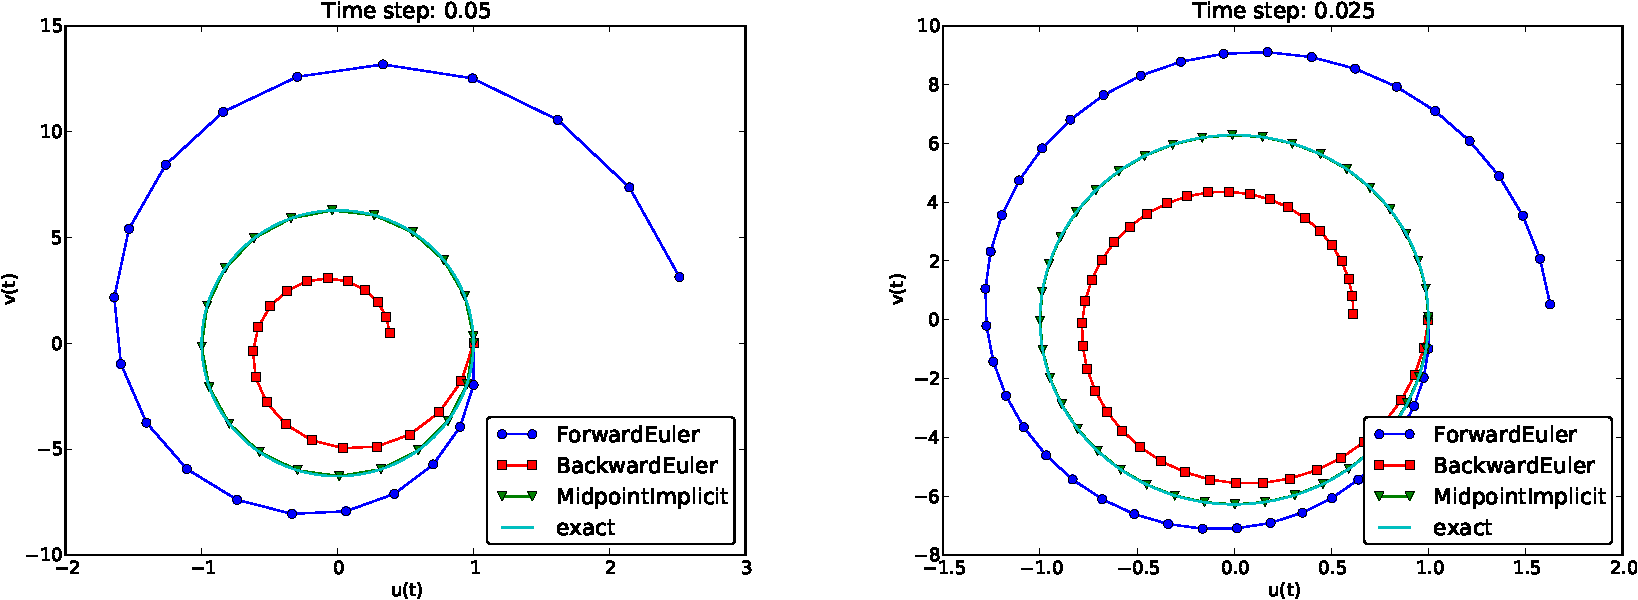
\includegraphics[width=1.0\linewidth]{fig-vib/vib_theta_1_pp.pdf}}
  \caption{
  Comparison of classical schemes in the phase plane for two time step values. \label{vib:ode1:1st:odespy:theta:phaseplane}
  }
\end{figure}
%\clearpage % flush figures vib:ode1:1st:odespy:theta:phaseplane



\begin{figure}[!ht]  % vib:ode1:1st:odespy:theta
  \centerline{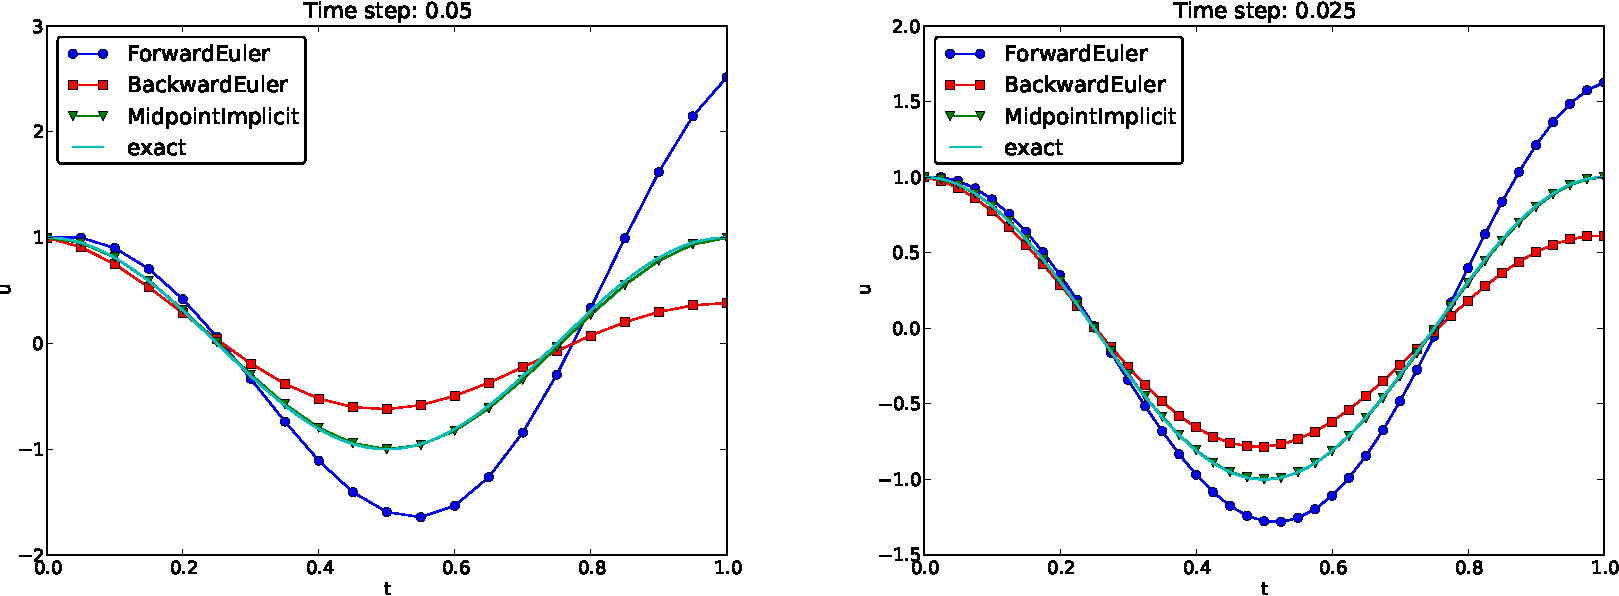
\includegraphics[width=1.0\linewidth]{fig-vib/vib_theta_1_u.pdf}}
  \caption{
  Comparison of solution curves for classical schemes. \label{vib:ode1:1st:odespy:theta}
  }
\end{figure}
%\clearpage % flush figures vib:ode1:1st:odespy:theta



\subsection{Runge-Kutta methods}

We may run two popular standard methods for first-order ODEs, the 2nd-
and 4th-order Runge-Kutta methods, to see how they perform. Figures~\ref{vib:ode1:1st:odespy:RK:phaseplane} and~\ref{vib:ode1:1st:odespy:RK} show the solutions with larger $\Delta
t$ values than what was used in the previous two plots.


\begin{figure}[!ht]  % vib:ode1:1st:odespy:RK:phaseplane
  \centerline{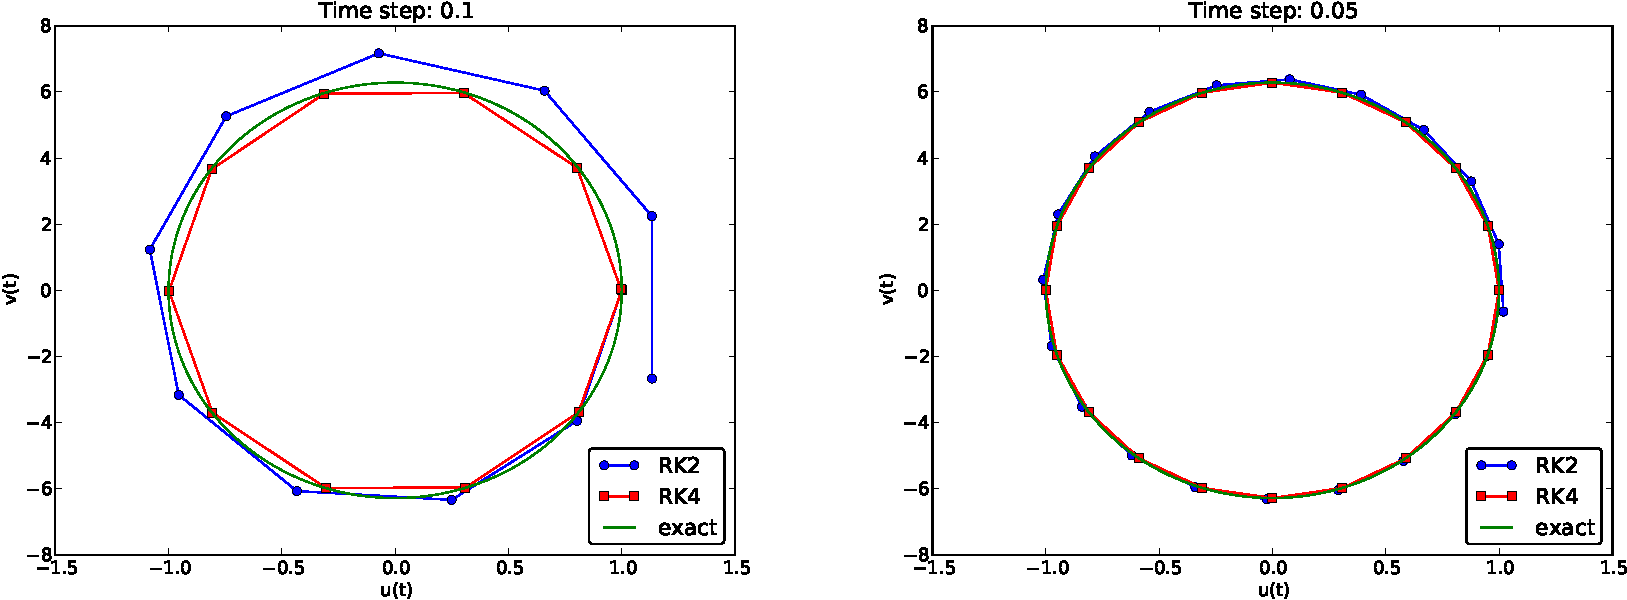
\includegraphics[width=1.0\linewidth]{fig-vib/vib_RK_1_pp.pdf}}
  \caption{
  Comparison of Runge-Kutta schemes in the phase plane. \label{vib:ode1:1st:odespy:RK:phaseplane}
  }
\end{figure}
%\clearpage % flush figures vib:ode1:1st:odespy:RK:phaseplane



\begin{figure}[!ht]  % vib:ode1:1st:odespy:RK
  \centerline{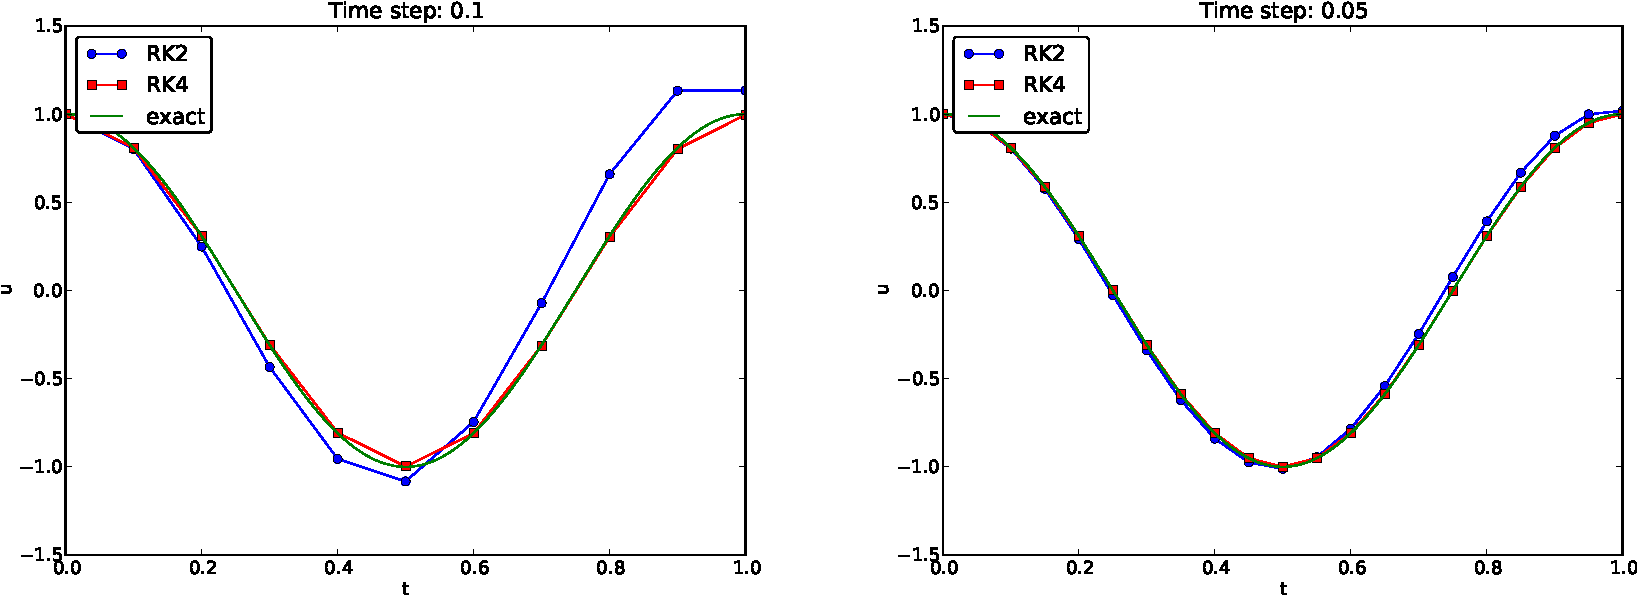
\includegraphics[width=1.0\linewidth]{fig-vib/vib_RK_1_u.pdf}}
  \caption{
  Comparison of Runge-Kutta schemes. \label{vib:ode1:1st:odespy:RK}
  }
\end{figure}
%\clearpage % flush figures vib:ode1:1st:odespy:RK



The visual impression is that the
4th-order Runge-Kutta method is very accurate, under all circumstances
in these tests, while the 2nd-order scheme suffers from amplitude errors
unless the time step is very small.


The corresponding results for the Crank-Nicolson scheme are shown in
Figure~\ref{vib:ode1:1st:odespy:CN:long:phaseplane}.
It is clear that the Crank-Nicolson
scheme outperforms the 2nd-order Runge-Kutta method. Both schemes have
the same order of accuracy $\Oof{\Delta t^2}$, but their differences
in the accuracy that matters in a real physical application is very
clearly pronounced in this example.  Exercise~\ref{vib:exer:undamped:odespy} invites you to investigate how the amplitude
is computed by a series of famous methods for first-order ODEs.


\begin{figure}[!ht]  % vib:ode1:1st:odespy:CN:long:phaseplane
  \centerline{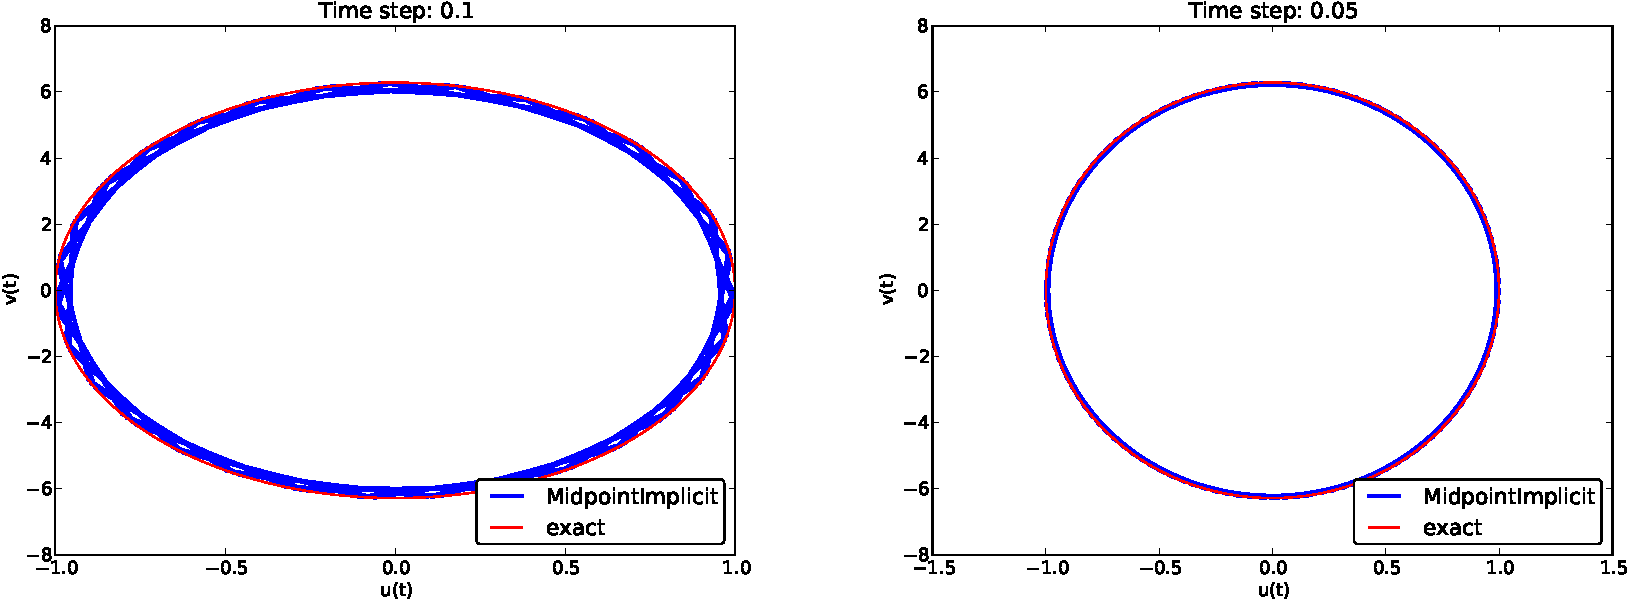
\includegraphics[width=1.0\linewidth]{fig-vib/vib_CN_10_pp.pdf}}
  \caption{
  Long-time behavior of the Crank-Nicolson scheme in the phase plane. \label{vib:ode1:1st:odespy:CN:long:phaseplane}
  }
\end{figure}
%\clearpage % flush figures vib:ode1:1st:odespy:CN:long:phaseplane




\subsection{Analysis of the Forward Euler scheme}

We may try to find exact solutions of the discrete
equations (\ref{vib:undamped:FE1})-(\ref{vib:undamped:FE2})
in the Forward Euler method. An ``ansatz''
is

\begin{align*}
u^n &= IA^n,\\ 
v^n &= qIA^n,
\end{align*}
where $q$ and $A$ are unknown numbers. We could have used a complex
exponential form $e^{i\tilde\omega n\Delta t}$ since we get
oscillatory form, but the oscillations grow in the Forward Euler
method, so the numerical frequency $\tilde\omega$ will be complex
anyway (producing an exponentially growing amplitude). Therefore, it is
easier to just work with potentially complex $A$ and $q$ as introduced
above.

The Forward Euler scheme leads to

\begin{align*}
A &= 1 + \Delta t q,\\ 
A &= 1 - \Delta t\omega^2 q^{-1}\tp
\end{align*}
We can easily eliminate $A$, get $q^2 + \omega^2=0$, and solve for

\[ q = \pm i\omega,\]
which gives

\[ A = 1 \pm \Delta t i\omega\tp\]
We shall take the real part of $A^n$ as the solution. The two
values of $A$ are complex conjugates, and the real part of
$A^n$ will be the same for both roots. This is easy to realize if
we rewrite the complex numbers in polar form,
which is also convenient
for further analysis and understanding.
The polar form $re^{i\theta}$ of a complex number $x+iy$ has
$r=\sqrt{x^2+y^2}$ and $\theta = \tan^{-1}(y/x)$.
Hence, the polar form of the two values for $A$ become

\[ 1 \pm \Delta t i\omega = \sqrt{1+\omega^2\Delta t^2}e^{\pm i\tan^{-1}(\omega\Delta t)}\tp\]
Now it is very easy to compute $A^n$:

\[ (1 \pm \Delta t i\omega)^n = (1+\omega^2\Delta t^2)^{n/2}e^{\pm ni\tan^{-1}(\omega\Delta t)}\tp\]
Since $\cos (\theta n) = \cos (-\theta n)$, the real part of the two
numbers become the same. We therefore continue with the solution that has
the plus sign.

The general solution is $u^n = CA^n$, where
$C$ is a constant determined from the initial condition:
$u^0=C=I$. We have $u^n=IA^n$ and
$v^n=qIA^n$. The final solutions
are just the real part of the expressions in polar form:

\begin{align}
u^n & =
I(1+\omega^2\Delta t^2)^{n/2}\cos (n\tan^{-1}(\omega\Delta t)),\\ 
v^n &=- \omega
I(1+\omega^2\Delta t^2)^{n/2}\sin (n\tan^{-1}(\omega\Delta t))\tp
\end{align}
The expression $(1+\omega^2\Delta t^2)^{n/2}$ causes growth of
the amplitude, since a number greater than one is raised to a positive
exponent $n/2$. We can develop a series expression to better understand
the formula for the amplitude. Introducing $p=\omega\Delta t$ as the
key variable and using \texttt{sympy} gives

\begin{cod}{cbg_blue1}\begin{Verbatim}[numbers=none,fontsize=\fontsize{9pt}{9pt},baselinestretch=0.95,xleftmargin=2mm]
>>> from sympy import *
>>> p = symbols('p', real=True)
>>> n = symbols('n', integer=True, positive=True)
>>> amplitude = (1 + p**2)**(n/2)
>>> amplitude.series(p, 0, 4)
1 + n*p**2/2 + O(p**4)
\end{Verbatim}
\end{cod}
\noindent
The amplitude goes like $1 + \half n\omega^2\Delta t^2$, clearly growing
linearly in time (with $n$).

We can also investigate the error in the angular frequency by a
series expansion:

\begin{cod}{cbg_blue1}\begin{Verbatim}[numbers=none,fontsize=\fontsize{9pt}{9pt},baselinestretch=0.95,xleftmargin=2mm]
>>> n*atan(p).series(p, 0, 4)
n*(p - p**3/3 + O(p**4))
\end{Verbatim}
\end{cod}
\noindent
This means that the solution for $u^n$ can be written as

\[ u^n = (1 + \half n\omega^2\Delta t^2 + \Oof(\Delta t^4))
\cos\left(\omega t - \frac{1}{3}\omega t\Delta t^2 + \Oof{\Delta t^4}\right)
\tp\]
The error in the angular frequency is of the same order as in the
scheme (\ref{vib:ode1:step4}) for the second-order ODE, but error
in the amplitude is severe.


\section{Energy considerations}
\label{vib:model1:energy}

\index{mechanical energy} \index{energy principle}

The observations of various methods in the previous section can be
better interpreted if we compute a quantity reflecting
the total \emph{energy of the system}. It turns out that this quantity,

\[ E(t) = \half(u^{\prime})^2 + \half\omega^2u^2,\]
is \emph{constant} for all $t$. Checking that $E(t)$ really remains constant
brings evidence that the numerical computations are sound.
It turns out that $E$ is proportional to the mechanical energy
in the system. Conservation of energy is
much used to check numerical simulations.

\subsection{Derivation of the energy expression}

We start out with multiplying

\[ u^{\prime\prime} + \omega^2 u = 0,\]
by $u^{\prime}$ and integrating from $0$ to $T$:

\[ \int_0^T u^{\prime\prime}u^{\prime} dt + \int_0^T\omega^2 u u^{\prime} dt = 0\tp\]
Observing that

\[ u^{\prime\prime}u^{\prime} = \frac{d}{dt}\half(u^{\prime})^2,\quad uu^{\prime} = \frac{d}{dt} {\half}u^2,\]
we get

\[
\int_0^T (\frac{d}{dt}\half(u^{\prime})^2 + \frac{d}{dt} \half\omega^2u^2)dt = E(T) - E(0)=0,
\]
where we have introduced

\begin{equation}
E(t) = \half(u^{\prime})^2 + \half\omega^2u^2\tp
\label{vib:model1:energy:balance1}
\end{equation}
The important result from this derivation is that the total energy
is constant:

\[ E(t) = E(0)\tp\]


\begin{warning_mdfboxadmon}[$E(t)$ is closely related to the system's energy.]
The quantity $E(t)$ derived above is physically not the mechanical energy of a
vibrating mechanical system, but the energy per unit mass. To see this,
we start with Newton's second law $F=ma$ ($F$ is the sum of forces, $m$
is the mass of the system, and $a$ is the acceleration).
The displacement $u$ is related to $a$ through
$a=u^{\prime\prime}$. With a spring force as the only force we have $F=-ku$, where
$k$ is a spring constant measuring the stiffness of the spring.
Newton's second law then implies the differential equation

\[ -ku = mu^{\prime\prime}\quad\Rightarrow mu^{\prime\prime} + ku = 0\tp\]
This equation of motion can be turned into an energy balance equation
by finding the work done by each term during a time interval $[0,T]$.
To this end, we multiply the equation by $du=u^{\prime}dt$ and integrate:

\[ \int_0^T muu^{\prime}dt + \int_0^T kuu^{\prime}dt = 0\tp\]
The result is

\[ \tilde E(t) = E_k(t) + E_p(t) = 0,\]
where

\begin{equation}
E_k(t) = \frac{1}{2}mv^2,\quad v=u^{\prime},
\label{vib:model1:energy:kinetic}
\end{equation}
is the \emph{kinetic energy} of the system, and

\begin{equation}
E_p(t) = {\half}ku^2
\label{vib:model1:energy:potential}
\end{equation}
is the \emph{potential energy}. The sum $\tilde E(t)$ is the total mechanical energy.
The derivation demonstrates the famous energy principle that, under
the right physical circumstances, any
change in the kinetic energy is due to a change in potential energy
and vice versa. (This principle breaks down when we introduce damping
in system, as we do in Section~\ref{vib:model2}.)

The equation $mu^{\prime\prime}+ku=0$ can be divided by $m$ and written as
$u^{\prime\prime} + \omega^2u=0$ for $\omega=\sqrt{k/m}$. The energy expression
$E(t)=\half(u^{\prime})^2 + \half\omega^2u^2$ derived earlier is then
$\tilde E(t)/m$, i.e., mechanical energy per unit mass.
\end{warning_mdfboxadmon}



\paragraph{Energy of the exact solution.}
Analytically, we have $u(t)=I\cos\omega t$, if $u(0)=I$ and $u^{\prime}(0)=0$,
so we can easily check that the energy evolution and confirm that $E(t)$
is constant:

\[ E(t) = {\half}I^2 (-\omega\sin\omega t)^2
+ \half\omega^2 I^2 \cos^2\omega t
= \half\omega^2 (\sin^2\omega t + \cos^2\omega t) = \half\omega^2
\tp
\]


\subsection{An error measure based on energy}

The constant energy is well expressed by its initial value $E(0)$, so that
the error in mechanical energy can be computed as a mesh function by

\begin{equation}
e_E^n = \half\left(\frac{u^{n+1}-u^{n-1}}{2\Delta t}\right)^2
+ \half\omega^2 (u^n)^2 - E(0),
\quad n=1,\ldots,N_t-1,
\end{equation}
where

\[ E(0) = {\half}V^2 + \half\omega^2I^2,\]
if $u(0)=I$ and $u^{\prime}(0)=V$. Note that we have used
a centered approximation to $u^{\prime}$: $\u^{\prime}(t_n)\approx
[D_{2t}u]^n$.

A useful norm of the mesh function $e_E^n$
for the discrete mechanical energy
can be the maximum absolute value of $e_E^n$:

\[ ||e_E^n||_{\ell^\infty} = \max_{1\leq n <N_t} |e_E^n|\tp\]
Alternatively, we can compute other norms involving integration over
all mesh points, but we are often interested in worst case deviation
of the energy, and then the maximum value is of particular relevance.

A vectorized Python implementation takes the form

\begin{cod}{cbg_blue1}\begin{Verbatim}[numbers=none,fontsize=\fontsize{9pt}{9pt},baselinestretch=0.95,xleftmargin=2mm]
# import numpy as np and compute u, t
dt = t[1]-t[0]
E = 0.5*((u[2:] - u[:-2])/(2*dt))**2 + 0.5*w**2*u[1:-1]**2
E0 = 0.5*V**2 + 0.5**w**2*I**2
e_E = E - E0
e_E_norm = np.abs(e_E).max()
\end{Verbatim}
\end{cod}
\noindent

The convergence rates of the quantity \Verb!e_E_norm! can be used for verification.
The value of \Verb!e_E_norm! is also useful for comparing schemes
through their ability to preserve energy. Below is a table demonstrating
the error in total energy for various schemes. We clearly see that
the Crank-Nicolson and 4th-order Runge-Kutta schemes are superior to
the 2nd-order Runge-Kutta method and better compared to the Forward
and Backward Euler schemes.


\begin{center}
\begin{tabular}{llll}
\hline
\multicolumn{1}{c}{ Method } & \multicolumn{1}{c}{ $T$ } & \multicolumn{1}{c}{ $\Delta t$ } & \multicolumn{1}{c}{ $\max \left\vert e_E^n\right\vert$ } \\
\hline
Forward Euler         & $1$  & $0.05$     & $1.113\cdot 10^{2}$                \\
Forward Euler         & $1$  & $0.025$    & $3.312\cdot 10^{1}$                \\
Backward Euler        & $1$  & $0.05$     & $1.683\cdot 10^{1}$                \\
Backward Euler        & $1$  & $0.025$    & $1.231\cdot 10^{1}$                \\
Runge-Kutta 2nd-order & $1$  & $0.1$      & $8.401$                            \\
Runge-Kutta 2nd-order & $1$  & $0.05$     & $9.637\cdot 10^{-1}$               \\
Crank-Nicolson        & $1$  & $0.05$     & $9.389\cdot 10^{-1}$               \\
Crank-Nicolson        & $1$  & $0.025$    & $2.411\cdot 10^{-1}$               \\
Runge-Kutta 4th-order & $1$  & $0.1$      & $2.387$                            \\
Runge-Kutta 4th-order & $1$  & $0.05$     & $6.476\cdot 10^{-1}$               \\
Crank-Nicolson        & $10$ & $0.1$      & $3.389$                            \\
Crank-Nicolson        & $10$ & $0.05$     & $9.389\cdot 10^{-1}$               \\
Runge-Kutta 4th-order & $10$ & $0.1$      & $3.686$                            \\
Runge-Kutta 4th-order & $10$ & $0.05$     & $6.928\cdot 10^{-1}$               \\
\hline
\end{tabular}
\end{center}

\noindent
\longinlinecomment{hpl 6}{ The error reductions are not directly in accordance with the order of the schemes, probably caused by $\Delta t$ not being in the asympotic regime. }{ The error reductions are }

% Should build a verification test on the energy error.

% Link phase plane plot to energy
% A phase plane plot shows the curve $(u(t), u^{\prime}(t))$.


\section{The Euler-Cromer method}
\label{vib:model2x2:EulerCromer}

While the 4th-order Runge-Kutta method and a
Crank-Nicolson scheme work well for vibration equation modeled as a
first-order ODE system,
both were inferior to the straightforward centered
difference scheme for the second-order equation
$u^{\prime\prime}+\omega^2u=0$. However, there is a similarly successful scheme
available for the first-order system $u^{\prime}=v$, $v'=-\omega^2u$, to be
presented next.

\index{forward-backward Euler-Cromer scheme}

\subsection{Forward-backward discretization}

The idea is to apply a Forward Euler discretization to the first
equation and a Backward Euler discretization to the second. In operator
notation this is stated as

\begin{align}
\lbrack D_t^+u &= v\rbrack^n,\\ 
\lbrack D_t^-v &= -\omega u\rbrack^{n+1}
\tp
\end{align}
We can write out the formulas and collect the unknowns on the left-hand side:
\begin{align}
u^{n+1} &= u^n + \Delta t v^n,
\label{vib:model2x2:EulerCromer:ueq1}\\ 
v^{n+1} &= v^n -\Delta t \omega^2u^{n+1}
\label{vib:model2x2:EulerCromer:veq1}
\tp
\end{align}
We realize that after $u^{n+1}$ has been computed from
(\ref{vib:model2x2:EulerCromer:ueq1}), it may be used directly
in
(\ref{vib:model2x2:EulerCromer:veq1}) to compute $v^{n+1}$.

In physics, it is more common to update the $v$ equation first, with
a forward difference, and thereafter the $u$ equation, with a backward
difference that applies the most recently computed $v$ value:

\begin{align}
v^{n+1} &= v^n -\Delta t \omega^2u^{n},
\label{vib:model2x2:EulerCromer:veq1b}\\ 
u^{n+1} &= u^n + \Delta t v^{n+1}\tp
\label{vib:model2x2:EulerCromer:ueq1b}
\end{align}
The advantage of ordering the ODEs as in
(\ref{vib:model2x2:EulerCromer:veq1b})-(\ref{vib:model2x2:EulerCromer:ueq1b})
becomes evident
when consider complicated models. Such models are included if
we write our vibration ODE more generally as

\[ \ddot u + g(u, u^{\prime}, t)=0\tp\]
We can rewrite this second-order ODE as two first-order ODEs,

\begin{align*}
v' &= -g(u,v,t),\\ 
u^{\prime} &= v\tp
\end{align*}
This rewrite allows the following scheme to be used:

\begin{align*}
v^{n+1} &= v^n -\Delta t\, g(u^n,v^n,t),\\ 
u^{n+1} &= u^n + \Delta t\, v^{n+1}\tp
\end{align*}
We realize that the first update works well with any $g$ since old
values $u^n$ and $v^n$ are used. Switching the equations would
demand $u^n{+1}$ and $v^{n+1}$ values in $g$.



% Despite using a backward difference, there is no need to solve a coupled
% system for $u^{n+1}$ and $v^{n+1}$ because the structure of the ODEs
% allows (\ref{vib:model2x2:EulerCromer:ueq1})

The scheme
(\ref{vib:model2x2:EulerCromer:veq1b})-(\ref{vib:model2x2:EulerCromer:ueq1b})
goes under several names: forward-backward scheme, \href{{http://en.wikipedia.org/wiki/Semi-implicit_Euler_method}}{semi-implicit Euler method}, semi-explicit Euler,
symplectic Euler,
Newton-St\"{o}rmer-Verlet,
and Euler-Cromer.
We shall stick to the latter name.
Since both time discretizations are based on first-order difference
approximation, one may think that the scheme is only of first-order,
but this is not true: the use of a forward and then a backward
difference make errors cancel so that the overall error in the scheme
is $\Oof{\Delta t^2}$. This is explained below.

\subsection{Equivalence with the scheme for the second-order ODE}
\label{vib:model2x2:EulerCromer:equiv}

We may eliminate the $v^n$ variable from
(\ref{vib:model2x2:EulerCromer:ueq1})-(\ref{vib:model2x2:EulerCromer:veq1})
or
(\ref{vib:model2x2:EulerCromer:veq1b})-(\ref{vib:model2x2:EulerCromer:ueq1b}).
The $v^{n+1}$ term in (\ref{vib:model2x2:EulerCromer:veq1b}) can
be eliminated from (\ref{vib:model2x2:EulerCromer:ueq1b}):
\begin{equation}
u^{n+1} = u^n + \Delta t (v^n - \omega^2\Delta t^2 u^n)\tp
\label{vib:model2x2:EulerCromer:elim1}
\end{equation}
The $v^{n}$ quantity can be expressed by $u^n$ and $u^{n-1}$
using (\ref{vib:model2x2:EulerCromer:ueq1b}):
\[ v^{n} = \frac{u^n - u^{n-1}}{\Delta t},
\]
and when this is inserted in (\ref{vib:model2x2:EulerCromer:elim1}) we get
\begin{equation}
u^{n+1} = 2u^n - u^{n-1} - \Delta t^2 \omega^2u^{n},
\end{equation}
which is nothing but the centered scheme (\ref{vib:ode1:step4})!
The two seemingly different numerical methods are mathematically
equivalent. Consequently,
the previous analysis of
(\ref{vib:ode1:step4}) also applies to the Euler-Cromer
method. In particular, the amplitude is constant, given that the stability
criterion is fulfilled, but there is always an angular frequency error
(\ref{vib:ode1:tildeomega:series}). Exercise~\ref{vib:exer:EulerCromer:analysis}
gives guidance on how to derive the exact discrete solution of
the two equations in the Euler-Cromer method.

Although the Euler-Cromer scheme and the method (\ref{vib:ode1:step4}) are
equivalent, there could be differences in the way they handle
the initial conditions. Let is look into this topic.
The initial condition $u^{\prime}=0$ means $u^{\prime}=v=0$.  From
(\ref{vib:model2x2:EulerCromer:ueq1b}) we get $v^1=-\omega^2 u^0$
and $u^1=u^0 - \omega^2\Delta t^2 u^0$. When using
a centered approximation of $u^{\prime}(0)=0$ combined with the
discretization (\ref{vib:ode1:step4}) of the second-order ODE, we
get $u^1=u^0 - \frac{1}{2}\omega^2\Delta t^2 u^0$. The difference
is $\frac{1}{2}\omega^2\Delta t^2 u^0$, which is of second order in $\Delta t$,
seemingly
consistent with the overall error in the scheme for the differential equation
model.

A different view can also be taken.
If we approximate $u^{\prime}(0)=0$ by a backward difference,
$(u^0-u^{-1})/\Delta t =0$, we get $u^{-1}=u^0$, and when combined
with (\ref{vib:ode1:step4}), it results in
$u^1=u^0 - \omega^2\Delta t^2 u^0$. This means that
the Euler-Cromer method based on
(\ref{vib:model2x2:EulerCromer:ueq1b})-(\ref{vib:model2x2:EulerCromer:veq1b})
corresponds to using only a first-order approximation to the initial condition
in the method from Section~\ref{vib:ode1:fdm}.

Correspondingly, using the formulation
(\ref{vib:model2x2:EulerCromer:ueq1})-(\ref{vib:model2x2:EulerCromer:veq1})
with $v^n=0$ leads to $u^1=u^0$, which can be interpreted as using
a forward difference approximation for the initial condition $u^{\prime}(0)=0$.
Both Euler-Cromer formulations lead to slightly different values for
$u^1$ compared to the method in Section~\ref{vib:ode1:fdm}.
The error is $\frac{1}{2}\omega^2\Delta t^2 u^0$ and of the same order
as the overall scheme.


\subsection{Implementation}
\label{vib:model2x2:EulerCromer:impl}

The function below, found in \href{{http://tinyurl.com/nm5587k/vib/vib_EulerCromer.py}}{\nolinkurl{vib_EulerCromer.py}} implements the Euler-Cromer scheme
(\ref{vib:model2x2:EulerCromer:veq1b})-(\ref{vib:model2x2:EulerCromer:ueq1b}):

\begin{cod}{cbg_blue1}\begin{Verbatim}[numbers=none,fontsize=\fontsize{9pt}{9pt},baselinestretch=0.95,xleftmargin=2mm]
import numpy as np

def solver(I, w, dt, T):
    """
    Solve v' = - w**2*u, u'=v for t in (0,T], u(0)=I and v(0)=0,
    by an Euler-Cromer method.
    """
    dt = float(dt)
    Nt = int(round(T/dt))
    u = np.zeros(Nt+1)
    v = np.zeros(Nt+1)
    t = np.linspace(0, Nt*dt, Nt+1)

    v[0] = 0
    u[0] = I
    for n in range(0, Nt):
        v[n+1] = v[n] - dt*w**2*u[n]
        u[n+1] = u[n] + dt*v[n+1]
    return u, v, t
\end{Verbatim}
\end{cod}
\noindent

Since the Euler-Cromer scheme is equivalent to the finite difference
method for the second-order ODE $u^{\prime\prime}+\omega^2u=0$ (see Section~\ref{vib:model2x2:EulerCromer:equiv}), the performance of the above
\texttt{solver} function is the same as for the \texttt{solver} function in Section~\ref{vib:impl1}. The only difference is the formula for the first time
step, as discussed above.  This deviation in the Euler-Cromer scheme
means that the discrete solution listed in Section~\ref{vib:ode1:analysis:sol} is not a solution of the Euler-Cromer
scheme!

To verify the implementation of the Euler-Cromer method we
can adjust \texttt{v[1]} so that the computer-generated values can be
compared with the formula
(\ref{vib:ode1:un:exact}) from in Section~\ref{vib:ode1:analysis:sol}. This
adjustment is done in an alternative solver function, \Verb!solver_ic_fix!
in \Verb!vib_EulerCromer.py!. Since we now have an exact solution of the
discrete equations available, we can write a test function
\Verb!test_solver! for checking the equality of computed values with the
formula (\ref{vib:ode1:un:exact}):

\begin{cod}{cbg_blue1}\begin{Verbatim}[numbers=none,fontsize=\fontsize{9pt}{9pt},baselinestretch=0.95,xleftmargin=2mm]
def test_solver():
    """
    Test solver with fixed initial condition against
    equivalent scheme for the 2nd-order ODE u'' + u = 0.
    """
    I = 1.2; w = 2.0; T = 5
    dt = 2/w  # longest possible time step
    u, v, t = solver_ic_fix(I, w, dt, T)
    from vib_undamped import solver as solver2  # 2nd-order ODE
    u2, t2 = solver2(I, w, dt, T)
    error = np.abs(u - u2).max()
    tol = 1E-14
    assert error < tol
\end{Verbatim}
\end{cod}
\noindent

Another function, \texttt{demo},
visualizes the difference between Euler-Cromer scheme and the scheme
(\ref{vib:ode1:step4})
for the second-oder ODE, arising from the mismatch in the first time level.

\shortinlinecomment{hpl 7}{ Odespy's Euler-Cromer, but it needs more work with the example code. }{ Odespy's Euler-Cromer, but it }

% is anything gained? is v of higher order than D_2t u from the
% other approach, i.e., if we need v, is this alg better? Probably not
% since v is related u through a difference

% make exercises:
% investigate how important the u^1 wrong formula really is on
% convergence rate

% new file: genealizations, systems,
% new file: apps

% exercise: damping analysis, see geophysics book first...

\subsection{The velocity Verlet algorithm}

Another very popular algorithm for vibration problems $u^{\prime\prime}+\omega^2u=0$
can be derived as follows. First, we step $u$ forward from $t_n$ to
$t_{n+1}$ using a three-term Taylor series,

\[ u(t_{n+1}) = u(t_n) + u^{\prime}(t_n)\Delta t + \frac{1}{2}u^{\prime\prime}(t_n)\Delta t^2\tp\]
Using $u^{\prime}=v$ and $u^{\prime\prime}=-\omega^2u$, we get the updating formula

\[ u^{n+1} = u^n + v^n\Delta t - \frac{1}{2}\Delta^2\omega^2u^n\tp\]
Second, the first-order equation for $v$,

\[ v'=-\omega^2u,\]
is discretized by a centered difference
in a Crank-Nicolson fashion at $t_{n+\frac{1}{2}}$:

\[ \frac{v^{n+1}-v^n}{\Delta t} = -\omega^2\frac{1}{2}(u^n + u^{n+1})\tp\]
To summarize, we have the scheme

\begin{align}
u^{n+1} &= u^n + v^n\Delta t - \frac{1}{2}\Delta^2\omega^2u^n
\label{vib:model2x2:Verlet:dueq} \\ 
v^{n+1} &= v^n -\frac{1}{2}\Delta t\omega^2 (u^n + u^{n+1}),
\label{vib:model2x2:Verlet:dveq}
\end{align}
known as the \emph{velocity Verlet} algorithm.
Observe that this scheme is explicit since $u^{n+1}$ in
(\ref{vib:model2x2:Verlet:dveq}) is already computed
from (\ref{vib:model2x2:Verlet:dueq}).

The algorithm can be straightforwardly implemented as shown below (the
code appears in the file \href{{http://tinyurl.com/nm5587k/vib/vib_undamped_velocity_Verlet.py}}{\nolinkurl{vib_undamped_velocity_Verlet.py}}).

\begin{cod}{cbg_blue1}\begin{Verbatim}[numbers=none,fontsize=\fontsize{9pt}{9pt},baselinestretch=0.95,xleftmargin=2mm]
from vib_undamped import convergence_rates, main

def solver(I, w, dt, T, return_v=False):
    """
    Solve u'=v, v'=-w**2*u for t in (0,T], u(0)=I and v(0)=0,
    by the velocity Verlet method with time step dt.
    """
    dt = float(dt)
    Nt = int(round(T/dt))
    u = np.zeros(Nt+1)
    v = np.zeros(Nt+1)
    t = np.linspace(0, Nt*dt, Nt+1)

    u[0] = I
    v[0] = 0
    for n in range(Nt):
        u[n+1] = u[n] + v[n]*dt - 0.5*dt**2*w**2*u[n]
        v[n+1] = v[n] - 0.5*dt*w**2*(u[n] + u[n+1])
    if return_v:
        return u, v, t
    else:
        # Return just u and t as in the vib_undamped.py's solver
        return u, t
\end{Verbatim}
\end{cod}
\noindent
We provide the option that this \texttt{solver} function returns the same data
as the \texttt{solver} function from Section~\ref{vib:impl1:solver} (if \Verb!return_v!
is \texttt{False}), but we may return \texttt{v} along with \texttt{u} and \texttt{t}.

The error in the Taylor series expansion behind
(\ref{vib:model2x2:Verlet:dueq}) is $\Oof{\Delta t^3}$, while the error
in the central difference for $v$ is $\Oof{\Delta t^2}$.  The overall
error is then no better than $\Oof{\Delta t^2}$, which can be verified
empirically using the \Verb!convergence_rates! function from~\ref{vib:ode1:verify}:

\begin{cod}{cbg_blue1}\begin{Verbatim}[numbers=none,fontsize=\fontsize{9pt}{9pt},baselinestretch=0.95,xleftmargin=2mm]
>>> import vib_undamped_velocity_Verlet as m
>>> m.convergence_rates(4, solver_function=m.solver)
[2.0036366687367346, 2.0009497328124835, 2.000240105995295]
\end{Verbatim}
\end{cod}
\noindent
% The output confirms that the overall convergence rate is 2.

% !split
\section{Generalization: damping, nonlinear spring, and external excitation}
\label{vib:model2}

\index{nonlinear restoring force}
\index{nonlinear spring}
\index{forced vibrations}

We shall now generalize the simple model problem from
Section~\ref{vib:model1} to include a possibly nonlinear damping term $f(u^{\prime})$,
a possibly nonlinear spring (or restoring) force $s(u)$, and
some external excitation $F(t)$:

\begin{equation}
mu^{\prime\prime} + f(u^{\prime}) + s(u) = F(t),\quad u(0)=I,\ u^{\prime}(0)=V,\ t\in (0,T]
\tp
\label{vib:ode2}
\end{equation}
We have also included a possibly nonzero initial value of $u^{\prime}(0)$.
The parameters $m$, $f(u^{\prime})$, $s(u)$, $F(t)$, $I$, $V$, and $T$ are
input data.

There are two main types of damping (friction) forces: linear $f(u^{\prime})=bu$, or
quadratic $f(u^{\prime})=bu^{\prime}|u^{\prime}|$. Spring systems often feature linear
damping, while air resistance usually gives rise to quadratic damping.
Spring forces are often linear: $s(u)=cu$, but nonlinear versions
are also common, the most famous is the gravity force on a pendulum
that acts as a spring with $s(u)\sim \sin(u)$.


\subsection{A centered scheme for linear damping}
\label{vib:ode2:fdm:flin}

Sampling (\ref{vib:ode2}) at a mesh point $t_n$, replacing
$u^{\prime\prime}(t_n)$ by $[D_tD_tu]^n$, and $u^{\prime}(t_n)$ by $[D_{2t}u]^n$ results
in the discretization

\begin{equation}
[mD_tD_t u + f(D_{2t}u) + s(u) = F]^n,
\end{equation}
which written out means

\begin{equation}
m\frac{u^{n+1}-2u^n + u^{n-1}}{\Delta t^2}
+ f(\frac{u^{n+1}-u^{n-1}}{2\Delta t}) + s(u^n) = F^n,
\label{vib:ode2:step3b}
\end{equation}
where $F^n$ as usual means $F(t)$ evaluated at $t=t_n$.
Solving (\ref{vib:ode2:step3b}) with respect to the unknown
$u^{n+1}$ gives a problem: the $u^{n+1}$ inside the $f$ function
makes the equation \emph{nonlinear} unless $f(u^{\prime})$ is a linear function,
$f(u^{\prime})=bu^{\prime}$. For now we shall assume that $f$ is linear in $u^{\prime}$.
Then

\begin{equation}
m\frac{u^{n+1}-2u^n + u^{n-1}}{\Delta t^2}
+ b\frac{u^{n+1}-u^{n-1}}{2\Delta t} + s(u^n) = F^n,
\label{vib:ode2:step3b2}
\end{equation}
which gives an explicit formula for $u$ at each
new time level:

\begin{equation}
u^{n+1} = (2mu^n + (\frac{b}{2}\Delta t - m)u^{n-1} +
\Delta t^2(F^n - s(u^n)))(m + \frac{b}{2}\Delta t)^{-1}
\label{vib:ode2:step4}
\tp
\end{equation}

For the first time step we need to discretize $u^{\prime}(0)=V$
as $[D_{2t}u = V]^0$ and combine
with (\ref{vib:ode2:step4}) for $n=0$. The discretized initial condition
leads to

\begin{equation}
u^{-1} = u^{1} - 2\Delta t V,
\label{vib:ode2:ic:du}
\end{equation}
which inserted in (\ref{vib:ode2:step4}) for $n=0$ gives an equation
that can be solved for
$u^1$:

\begin{equation}
u^1 = u^0 + \Delta t\, V
+ \frac{\Delta t^2}{2m}(-bV - s(u^0) + F^0)
\tp
\label{vib:ode2:step4b}
\end{equation}

\subsection{A centered scheme for quadratic damping}
\label{vib:ode2:fdm:fquad}

When $f(u^{\prime})=bu^{\prime}|u^{\prime}|$, we get a quadratic equation for $u^{n+1}$
in (\ref{vib:ode2:step3b}). This equation can be straightforwardly
solved by the well-known formula for the roots of a quadratic equation.
However, we can also avoid the nonlinearity by introducing
an approximation with an error of order no higher than what we
already have from replacing derivatives with finite differences.

\index{geometric mean}
\index{averaging!geometric}

We start with (\ref{vib:ode2}) and only replace
$u^{\prime\prime}$ by $D_tD_tu$, resulting in

\begin{equation}
[mD_tD_t u + bu^{\prime}|u^{\prime}| + s(u) = F]^n\tp
\label{vib:ode2:quad:idea1}
\end{equation}
Here, $u^{\prime}|u^{\prime}|$ is to be computed at time $t_n$. The idea
is now to introduce
a \emph{geometric mean}, defined by

\[ (w^2)^n \approx w^{n-\half}w^{n+\half},\]
for some quantity $w$ depending on time. The error in the geometric mean
approximation is $\Oof{\Delta t^2}$, the same as in the
approximation $u^{\prime\prime}\approx D_tD_tu$. With $w=u^{\prime}$ it follows
that

\[ [u^{\prime}|u^{\prime}|]^n \approx u^{\prime}(t_{n+\half})|u^{\prime}(t_{n-\half})|\tp\]
The next step is to approximate
$u^{\prime}$ at $t_{n\pm 1/2}$, and fortunately a centered difference
fits perfectly into the formulas since it involves $u$ values at
the mesh points only. With the approximations


\begin{equation}
u^{\prime}(t_{n+1/2})\approx [D_t u]^{n+\half},\quad u^{\prime}(t_{n-1/2})\approx [D_t u]^{n-\half},
\label{vib:ode2:quad:idea2}
\end{equation}
we get

\begin{equation}
[u^{\prime}|u^{\prime}|]^n
\approx [D_tu]^{n+\half}|[D_tu]^{n-\half}| = \frac{u^{n+1}-u^n}{\Delta t}
\frac{|u^n-u^{n-1}|}{\Delta t}
\tp
\end{equation}
The counterpart to (\ref{vib:ode2:step3b}) is then

\begin{equation}
m\frac{u^{n+1}-2u^n + u^{n-1}}{\Delta t^2}
+ b\frac{u^{n+1}-u^n}{\Delta t}\frac{|u^n-u^{n-1}|}{\Delta t}
+ s(u^n) = F^n,
\label{vib:ode2:step3b:quad}
\end{equation}
which is linear in the unknown $u^{n+1}$. Therefore, we can easily solve
(\ref{vib:ode2:step3b:quad})
with respect to $u^{n+1}$ and achieve the explicit updating formula

\begin{align}
u^{n+1} &=  \left( m + b|u^n-u^{n-1}|\right)^{-1}\times \nonumber\\ 
& \qquad \left(2m u^n - mu^{n-1} + bu^n|u^n-u^{n-1}| + \Delta t^2 (F^n - s(u^n))
\right)
\tp
\label{vib:ode2:step4:quad}
\end{align}

% Make exercise to solve complicated u^1 equation with Bisection/Newton

In the derivation of a special equation for the first
time step we run into some trouble: inserting (\ref{vib:ode2:ic:du})
in (\ref{vib:ode2:step4:quad}) for $n=0$ results in a complicated nonlinear
equation for $u^1$. By thinking differently about the problem we can
easily get away with the nonlinearity again. We have for $n=0$ that
$b[u^{\prime}|u^{\prime}|]^0 = bV|V|$. Using this value in (\ref{vib:ode2:quad:idea1})
gives

\begin{equation}
[mD_tD_t u + bV|V| + s(u) = F]^0
\tp
\end{equation}
Writing this equation out and using (\ref{vib:ode2:ic:du}) results in the
special equation for the first time step:

\begin{equation}
u^1 = u^0 + \Delta t V + \frac{\Delta t^2}{2m}\left(-bV|V| - s(u^0) + F^0\right)
\tp
\label{vib:ode2:step4b:quad}
\end{equation}

\subsection{A forward-backward discretization of the quadratic damping term}

The previous section first proposed to discretize the quadratic
damping term $|u^{\prime}|u^{\prime}$ using centered differences:
$[|D_{2t}|D_{2t}u]^n$. As this gives rise to a nonlinearity in
$u^{n+1}$, it was instead proposed to use a geometric mean combined
with centered differences.  But there are other alternatives. To get
rid of the nonlinearity in $[|D_{2t}|D_{2t}u]^n$, one can think
differently: apply a backward difference to $|u^{\prime}|$, such that
the term involves known values, and apply a forward difference to
$u^{\prime}$ to make the term linear in the unknown $u^{n+1}$. With
mathematics,

\begin{equation}
[\beta |u^{\prime}|u^{\prime}]^n \approx \beta |[D_t^-u]^n|[D_t^+ u]^n =
\beta\left\vert\frac{u^n-u^{n-1}}{\Delta t}\right\vert
\frac{u^{n+1}-u^n}{\Delta t}\tp
\label{vib:ode2:nonlin:fbdiff}
\end{equation}
The forward and backward differences have both an error proportional
to $\Delta t$ so one may think the discretization above leads to
a first-order scheme.
However, by looking at the formulas, we realize that the forward-backward
differences in (\ref{vib:ode2:nonlin:fbdiff})
result in exactly the same scheme as in
(\ref{vib:ode2:step3b:quad}) where we
used a geometric mean and centered differences and committed errors
of size $\Oof{\Delta t^2}$. Therefore, the forward-backward
differences in (\ref{vib:ode2:nonlin:fbdiff})
act in a symmetric way and actually produce a second-order
accurate discretization of the quadratic damping term.


\subsection{Implementation}
\label{vib:ode2:solver}

The algorithm arising from the methods in Sections~\ref{vib:ode2:fdm:flin}
and~\ref{vib:ode2:fdm:fquad} is very similar to the undamped case in
Section~\ref{vib:ode1:fdm}. The difference is
basically a question of different formulas for $u^1$ and
$u^{n+1}$. This is actually quite remarkable. The equation
(\ref{vib:ode2}) is normally impossible to solve by pen and paper, but
possible for some special choices of $F$, $s$, and $f$. On the
contrary, the complexity of the
nonlinear generalized model (\ref{vib:ode2}) versus the
simple undamped model is not a big deal when we solve the
problem numerically!

The computational algorithm takes the form

\begin{enumerate}
 \item $u^0=I$

 \item compute $u^1$ from (\ref{vib:ode2:step4b}) if linear
    damping or (\ref{vib:ode2:step4b:quad}) if quadratic damping

 \item for $n=1,2,\ldots,N_t-1$:
\begin{enumerate}

   \item compute $u^{n+1}$ from (\ref{vib:ode2:step4}) if linear
      damping or (\ref{vib:ode2:step4:quad}) if quadratic damping
\end{enumerate}

\noindent
\end{enumerate}

\noindent
Modifying the \texttt{solver} function for the undamped case is fairly
easy, the big difference being many more terms and if tests on
the type of damping:

\begin{cod}{cbg_blue1}\begin{Verbatim}[numbers=none,fontsize=\fontsize{9pt}{9pt},baselinestretch=0.95,xleftmargin=2mm]
def solver(I, V, m, b, s, F, dt, T, damping='linear'):
    """
    Solve m*u'' + f(u') + s(u) = F(t) for t in (0,T],
    u(0)=I and u'(0)=V,
    by a central finite difference method with time step dt.
    If damping is 'linear', f(u')=b*u, while if damping is
    'quadratic', f(u')=b*u'*abs(u').
    F(t) and s(u) are Python functions.
    """
    dt = float(dt); b = float(b); m = float(m) # avoid integer div.
    Nt = int(round(T/dt))
    u = np.zeros(Nt+1)
    t = np.linspace(0, Nt*dt, Nt+1)

    u[0] = I
    if damping == 'linear':
        u[1] = u[0] + dt*V + dt**2/(2*m)*(-b*V - s(u[0]) + F(t[0]))
    elif damping == 'quadratic':
        u[1] = u[0] + dt*V + \ 
               dt**2/(2*m)*(-b*V*abs(V) - s(u[0]) + F(t[0]))

    for n in range(1, Nt):
        if damping == 'linear':
            u[n+1] = (2*m*u[n] + (b*dt/2 - m)*u[n-1] +
                      dt**2*(F(t[n]) - s(u[n])))/(m + b*dt/2)
        elif damping == 'quadratic':
            u[n+1] = (2*m*u[n] - m*u[n-1] + b*u[n]*abs(u[n] - u[n-1])
                      + dt**2*(F(t[n]) - s(u[n])))/\ 
                      (m + b*abs(u[n] - u[n-1]))
    return u, t
\end{Verbatim}
\end{cod}
\noindent
The complete code resides in the file \href{{http://tinyurl.com/nm5587k/vib/vib.py}}{\nolinkurl{vib.py}}.

\subsection{Verification}
\label{vib:ode2:verify}

\paragraph{Constant solution.}
For debugging and initial verification, a constant solution is often
very useful. We choose $\uex(t)=I$, which implies $V=0$.
Inserted in the ODE, we get
$F(t)=s(I)$ for any choice of $f$. Since the discrete derivative
of a constant vanishes (in particular, $[D_{2t}I]^n=0$,
$[D_tI]^n=0$, and $[D_tD_t I]^n=0$), the constant solution also fulfills
the discrete equations. The constant should therefore be reproduced
to machine precision. The function \Verb!test_constant! in \texttt{vib.py}
implements this test.

\longinlinecomment{hpl 8}{ Add verification tests for constant, linear, quadratic. Check how many bugs that are caught by these tests. }{ Add verification tests for }

\paragraph{Linear solution.}
Now we choose a linear solution: $\uex = ct + d$. The initial condition
$u(0)=I$ implies $d=I$, and $u^{\prime}(0)=V$ forces $c$ to be $V$.
Inserting $\uex=Vt+I$ in the ODE with linear damping results in

\[ 0 + bV + s(Vt+I) = F(t),\]
while quadratic damping requires the source term

\[ 0 + b|V|V + s(Vt+I) = F(t)\tp\]
Since the finite difference approximations used to compute $u^{\prime}$ all
are exact for a linear function, it turns out that the linear $\uex$
is also a solution of the discrete equations.
Exercise~\ref{vib:exer:verify:gen:linear} asks you to carry out
all the details.

\paragraph{Quadratic solution.}
Choosing $\uex = bt^2 + Vt + I$, with $b$ arbitrary,
fulfills the initial conditions and
fits the ODE if $F$ is adjusted properly. The solution also solves
the discrete equations with linear damping. However, this quadratic
polynomial in $t$ does not fulfill the discrete equations in case
of quadratic damping, because the geometric mean used in the approximation
of this term introduces an error.
Doing Exercise~\ref{vib:exer:verify:gen:linear} will reveal
the details. One can fit $F^n$ in the discrete equations such that
the quadratic polynomial is reproduced by the numerical method (to
machine precision).

% More: classes, cases with pendulum approx u vs sin(u),
% making UI via parampool

\subsection{Visualization}
\label{vib:ode2:viz}

The functions for visualizations differ significantly from
those in the undamped case in the \Verb!vib_undamped.py! program because,
in the present general case, we do not have an exact solution to
include in the plots. Moreover, we have no good estimate of
the periods of the oscillations as there will be one period
determined by the system parameters, essentially the
approximate frequency $\sqrt{s'(0)/m}$ for linear $s$ and small damping,
and one period dictated by $F(t)$ in case the excitation is periodic.
This is, however,
nothing that the program can depend on or make use of.
Therefore, the user has to specify $T$ and the window width
to get a plot that moves with the graph and shows
the most recent parts of it in long time simulations.

The \texttt{vib.py} code
contains several functions for analyzing the time series signal
and for visualizing the solutions.

\subsection{User interface}
\label{vib:ode2:ui}

\index{ArgumentParser@{\rm\texttt{ArgumentParser}} (Python class)}
\index{argparse@{\rm\texttt{argparse}} (Python module)}

The \texttt{main} function is changed substantially from
the \Verb!vib_undamped.py! code, since we need to
specify the new data $c$, $s(u)$, and $F(t)$.  In addition, we must
set $T$ and the plot window width (instead of the number of periods we
want to simulate as in \Verb!vib_undamped.py!). To figure out whether we
can use one plot for the whole time series or if we should follow the
most recent part of $u$, we can use the \Verb!plot_empricial_freq_and_amplitude!
function's estimate of the number of local maxima. This number is now
returned from the function and used in \texttt{main} to decide on the
visualization technique.

\begin{cod}{cbg_blue1}\begin{Verbatim}[numbers=none,fontsize=\fontsize{9pt}{9pt},baselinestretch=0.95,xleftmargin=2mm]
def main():
    import argparse
    parser = argparse.ArgumentParser()
    parser.add_argument('--I', type=float, default=1.0)
    parser.add_argument('--V', type=float, default=0.0)
    parser.add_argument('--m', type=float, default=1.0)
    parser.add_argument('--c', type=float, default=0.0)
    parser.add_argument('--s', type=str, default='u')
    parser.add_argument('--F', type=str, default='0')
    parser.add_argument('--dt', type=float, default=0.05)
    parser.add_argument('--T', type=float, default=140)
    parser.add_argument('--damping', type=str, default='linear')
    parser.add_argument('--window_width', type=float, default=30)
    parser.add_argument('--savefig', action='store_true')
    a = parser.parse_args()
    from scitools.std import StringFunction
    s = StringFunction(a.s, independent_variable='u')
    F = StringFunction(a.F, independent_variable='t')
    I, V, m, c, dt, T, window_width, savefig, damping = \ 
       a.I, a.V, a.m, a.c, a.dt, a.T, a.window_width, a.savefig, \ 
       a.damping

    u, t = solver(I, V, m, c, s, F, dt, T)
    num_periods = empirical_freq_and_amplitude(u, t)
    if num_periods <= 15:
        figure()
        visualize(u, t)
    else:
        visualize_front(u, t, window_width, savefig)
    show()
\end{Verbatim}
\end{cod}
\noindent
The program \texttt{vib.py} contains
the above code snippets and can solve the model problem
(\ref{vib:ode2}). As a demo of \texttt{vib.py}, we consider the case
$I=1$, $V=0$, $m=1$, $c=0.03$, $s(u)=\sin(u)$, $F(t)=3\cos(4t)$,
$\Delta t = 0.05$, and $T=140$. The relevant command to run is

\begin{Verbatim}[frame=lines,label=\fbox{{\tiny Terminal}},framesep=2.5mm,framerule=0.7pt,fontsize=\fontsize{9pt}{9pt}]
Terminal> python vib.py --s 'sin(u)' --F '3*cos(4*t)' --c 0.03
\end{Verbatim}
This results in a \href{{http://tinyurl.com/opdfafk/pub/mov-vib/vib_generalized_dt0.05/index.html}}{moving window following the function} on the screen.
Figure~\ref{vib:ode2:fig:demo} shows a part of the time series.


\begin{figure}[!ht]  % vib:ode2:fig:demo
  \centerline{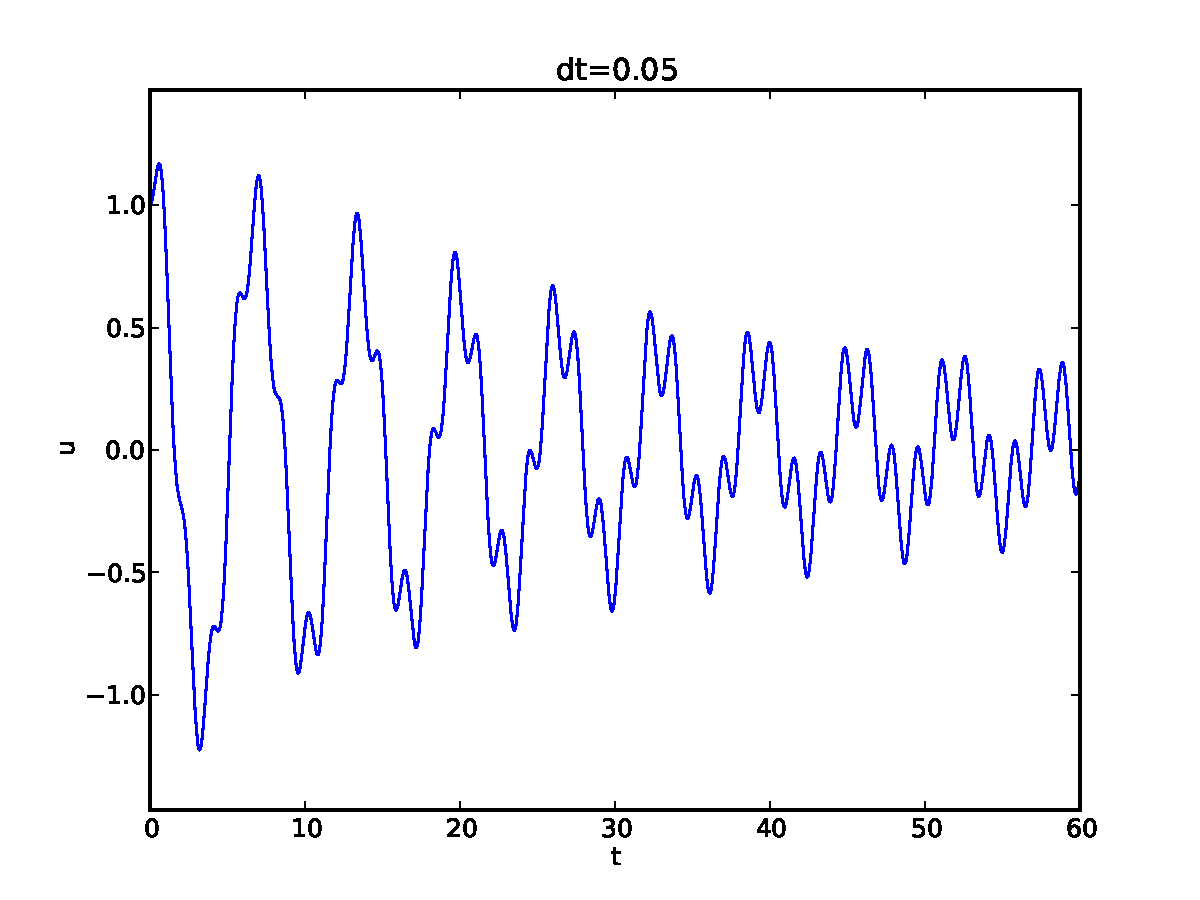
\includegraphics[width=1.0\linewidth]{fig-vib/vib_gen_demo.pdf}}
  \caption{
  Damped oscillator excited by a sinusoidal function. \label{vib:ode2:fig:demo}
  }
\end{figure}
%\clearpage % flush figures vib:ode2:fig:demo


\subsection{The Euler-Cromer scheme for the generalized model}

The ideas of the Euler-Cromer method from Section~\ref{vib:model2x2:EulerCromer}
carry over to the generalized model. We write (\ref{vib:ode2})
as two equations for $u$ and $v=u^{\prime}$. The first equation is taken as the
one with $v'$ on the left-hand side:

\begin{align}
v' &= \frac{1}{m}(F(t)-s(u)-f(v)),
\label{vib:ode2:EulerCromer:veq}\\ 
u^{\prime} &= v\tp
\label{vib:ode2:EulerCromer:ueq}
\end{align}
The idea is to step (\ref{vib:ode2:EulerCromer:veq}) forward using
a standard Forward Euler method, while we update $u$ from
(\ref{vib:ode2:EulerCromer:ueq}) with a Backward Euler method,
utilizing the recent, computed $v^{n+1}$ value. In detail,

\begin{align}
\frac{v^{n+1}-v^n}{\Delta t} &= \frac{1}{m}(F(t_n)-s(u^n)-f(v^n)),
\label{vib:ode2:EulerCromer:dveq0a}\\ 
\frac{u^{n+1}-u^n}{\Delta t} &= v^{n+1},
\label{vib:ode2:EulerCromer:dueq0a}
\end{align}
resulting in the explicit scheme

\begin{align}
v^{n+1} &= v^n + \Delta t\frac{1}{m}(F(t_n)-s(u^n)-f(v^n)),
\label{vib:ode2:EulerCromer:dveq}\\ 
u^{n+1} &= u^n + \Delta t\,v^{n+1}\tp
\label{vib:ode2:EulerCromer:dueq0}
\end{align}
We immediately note one very favorable feature of this scheme: all the
nonlinearities in $s(u)$ and $f(v)$ are evaluated at a previous time
level. This makes the Euler-Cromer method easier to apply and
hence much more convenient than the centered scheme for the second-order
ODE (\ref{vib:ode2}).

The initial conditions are trivially set as

\begin{align}
v^0 &= V,\\ 
u^0 &= I\tp
\end{align}

\shortinlinecomment{hpl 9}{ odespy for the generalized problem }{ odespy for the generalized }

\section{Exercises and Problems}



% --- begin exercise ---
\begin{doconceexercise}
\refstepcounter{doconceexercisecounter}

\subsection*{Problem \thedoconceexercisecounter: Use linear/quadratic functions for verification}

\label{vib:exer:undamped:verify:linquad}

Consider the ODE problem

\[ u^{\prime\prime} + \omega^2u=f(t), \quad u(0)=I,\ u^{\prime}(0)=V,\ t\in(0,T]\tp\]
Discretize this equation according to
$[D_tD_t u + \omega^2 u = f]^n$.


\subex{a)}
Derive the equation for the
first time step ($u^1$).

\subex{b)}
For verification purposes,
we use the method of manufactured solutions (MMS) with the
choice of $\uex(x,t)= ct+d$.
Find restrictions on $c$ and $d$ from
the initial conditions. Compute the corresponding source term $f$ by term.
Show that $[D_tD_t t]^n=0$ and use the fact
that the $D_tD_t$ operator is linear,
$[D_tD_t (ct+d)]^n = c[D_tD_t t]^n + [D_tD_t d]^n = 0$, to show that
$\uex$ is also a perfect solution of the discrete equations.

\subex{c)}
Use \texttt{sympy} to do the symbolic calculations above. Here is a
sketch of the program \Verb!vib_undamped_verify_mms.py!:

\begin{cod}{cbg_blue1}\begin{Verbatim}[numbers=none,fontsize=\fontsize{9pt}{9pt},baselinestretch=0.95,xleftmargin=2mm]
import sympy as sym
V, t, I, w, dt = sym.symbols('V t I w dt')  # global symbols
f = None  # global variable for the source term in the ODE

def ode_source_term(u):
    """Return the terms in the ODE that the source term
    must balance, here u'' + w**2*u.
    u is symbolic Python function of t."""
    return sym.diff(u(t), t, t) + w**2*u(t)

def residual_discrete_eq(u):
    """Return the residual of the discrete eq. with u inserted."""
    R = ...
    return sym.simplify(R)

def residual_discrete_eq_step1(u):
    """Return the residual of the discrete eq. at the first
    step with u inserted."""
    R = ...
    return sym.simplify(R)

def DtDt(u, dt):
    """Return 2nd-order finite difference for u_tt.
    u is a symbolic Python function of t.
    """
    return ...

def main(u):
    """
    Given some chosen solution u (as a function of t, implemented
    as a Python function), use the method of manufactured solutions
    to compute the source term f, and check if u also solves
    the discrete equations.
    """
    print '=== Testing exact solution: %s ===' % u
    print "Initial conditions u(0)=%s, u'(0)=%s:" % \ 
          (u(t).subs(t, 0), sym.diff(u(t), t).subs(t, 0))

    # Method of manufactured solution requires fitting f
    global f  # source term in the ODE
    f = sym.simplify(ode_lhs(u))

    # Residual in discrete equations (should be 0)
    print 'residual step1:', residual_discrete_eq_step1(u)
    print 'residual:', residual_discrete_eq(u)

def linear():
    main(lambda t: V*t + I)

if __name__ == '__main__':
    linear()
\end{Verbatim}
\end{cod}
\noindent
Fill in the various functions such that the calls in the \texttt{main}
function works.

\subex{d)}
The purpose now is to choose a quadratic function
$\uex = bt^2 + ct + d$ as exact solution. Extend the \texttt{sympy}
code above with a function \texttt{quadratic} for fitting \texttt{f} and checking
if the discrete equations are fulfilled. (The function is very similar
to \texttt{linear}.)

% Check with hand calculations that the \texttt{sympy} implementation
% is correct.

\subex{e)}
Will a polynomial of degree three fulfill the discrete equations?

\subex{f)}
Implement a \texttt{solver} function for computing the numerical
solution of this problem.


\subex{g)}
Write a nose test for checking that the quadratic solution
is computed to correctly (too machine precision, but the
round-off errors accumulate and increase with $T$) by the \texttt{solver}
function.


\noindent Filename: \Verb!vib_undamped_verify_mms!.

\end{doconceexercise}
% --- end exercise ---




% --- begin exercise ---
\begin{doconceexercise}
\refstepcounter{doconceexercisecounter}

\subsection*{Exercise \thedoconceexercisecounter: Show linear growth of the phase with time}

\label{vib:exer:phase:err:growth}

Consider an exact solution $I\cos (\omega t)$ and an
approximation $I\cos(\tilde\omega t)$.
Define the phase error as time lag between the peak $I$
in the exact solution and the corresponding peak in the approximation
after $m$ periods of oscillations. Show that this phase error
is linear in $m$.
\noindent Filename: \Verb!vib_phase_error_growth!.

\end{doconceexercise}
% --- end exercise ---




% --- begin exercise ---
\begin{doconceexercise}
\refstepcounter{doconceexercisecounter}

\subsection*{Exercise \thedoconceexercisecounter: Improve the accuracy by adjusting the frequency}

\label{vib:exer:w:adjust}

According to (\ref{vib:ode1:tildeomega:series}), the numerical
frequency deviates from the exact frequency by a (dominating) amount
$\omega^3\Delta t^2/24 >0$. Replace the \texttt{w} parameter in the algorithm
in the \texttt{solver} function in \Verb!vib_undamped.py! by \texttt{w*(1 - (1./24)*w**2*dt**2} and test how this adjustment in the numerical
algorithm improves the accuracy (use $\Delta t =0.1$ and simulate
for 80 periods, with and without adjustment of $\omega$).
\noindent Filename: \Verb!vib_adjust_w!.


% How does this go if
\end{doconceexercise}
% --- end exercise ---




% --- begin exercise ---
\begin{doconceexercise}
\refstepcounter{doconceexercisecounter}

\subsection*{Exercise \thedoconceexercisecounter: See if adaptive methods improve the phase error}

\label{vib:exer:undamped:adaptive}

Adaptive methods for solving ODEs aim at adjusting $\Delta t$ such
that the error is within a user-prescribed tolerance. Implement the
equation $u^{\prime\prime}+u=0$ in the \href{{https://github.com/hplgit/odespy}}{Odespy}
software. Use the example from Section~\ref{decay:fd2:adaptiveRK} in \cite{Langtangen_decay}.  Run the scheme with a very low
tolerance (say $10^{-14}$) and for a long time, check the number of
time points in the solver's mesh (\Verb!len(solver.t_all)!), and compare
the phase error with that produced by the simple finite difference
method from Section~\ref{vib:ode1:fdm} with the same number of (equally
spaced) mesh points. The question is whether it pays off to use an
adaptive solver or if equally many points with a simple method gives
about the same accuracy.
\noindent Filename: \Verb!vib_undamped_adaptive!.

\end{doconceexercise}
% --- end exercise ---




% --- begin exercise ---
\begin{doconceexercise}
\refstepcounter{doconceexercisecounter}

\subsection*{Exercise \thedoconceexercisecounter: Use a Taylor polynomial to compute $u^1$}

\label{vib:exer:step4b:alt}

As an alternative to the derivation of (\ref{vib:ode1:step4b}) for
computing $u^1$, one can use a Taylor polynomial with three terms
for $u^1$:

\[ u(t_1) \approx u(0) + u^{\prime}(0)\Delta t + {\half}u^{\prime\prime}(0)\Delta t^2\]
With $u^{\prime\prime}=-\omega^2 u$ and $u^{\prime}(0)=0$, show that this method also leads to
(\ref{vib:ode1:step4b}). Generalize the condition on $u^{\prime}(0)$ to
be $u^{\prime}(0)=V$ and compute $u^1$ in this case with both methods.
\noindent Filename: \Verb!vib_first_step!.

\end{doconceexercise}
% --- end exercise ---




% --- begin exercise ---
\begin{doconceexercise}
\refstepcounter{doconceexercisecounter}

\subsection*{Exercise \thedoconceexercisecounter: Find the minimal resolution of an oscillatory function}

\label{vib:exer:wdt:limit}

% Short: Find the largest relevant value of $\omega\Delta t$


Sketch the function on a given mesh which has the highest possible
frequency. That is, this oscillatory "cos-like" function has its
maxima and minima at every two grid points.  Find an expression for
the frequency of this function, and use the result to find the largest
relevant value of $\omega\Delta t$ when $\omega$ is the frequency
of an oscillating function and $\Delta t$ is the mesh spacing.
\noindent Filename: \Verb!vib_largest_wdt!.

\end{doconceexercise}
% --- end exercise ---




% --- begin exercise ---
\begin{doconceexercise}
\refstepcounter{doconceexercisecounter}

\subsection*{Exercise \thedoconceexercisecounter: Visualize the accuracy of finite differences for a cosine function}

\label{vib:exer:fd:exp:plot}

% Short: Visualize the accuracy of finite differences


We introduce the error fraction
\[ E = \frac{[D_tD_t u]^n}{u^{\prime\prime}(t_n)} \]
to measure the error in the finite difference approximation $D_tD_tu$ to
$u^{\prime\prime}$.
Compute $E$
for the specific choice of a cosine/sine function of the
form $u=\exp{(i\omega t)}$ and show that
\[ E = \left(\frac{2}{\omega\Delta t}\right)^2
\sin^2(\frac{\omega\Delta t}{2})
\tp
\]
Plot $E$ as a function of $p=\omega\Delta t$. The relevant
values of $p$ are $[0,\pi]$ (see Exercise~\ref{vib:exer:wdt:limit}
for why $p>\pi$ does not make sense).
The deviation of the curve from unity visualizes the error in the
approximation. Also expand $E$ as a Taylor polynomial in $p$ up to
fourth degree (use, e.g., \texttt{sympy}).
\noindent Filename: \Verb!vib_plot_fd_exp_error!.

\end{doconceexercise}
% --- end exercise ---




% --- begin exercise ---
\begin{doconceexercise}
\refstepcounter{doconceexercisecounter}

\subsection*{Exercise \thedoconceexercisecounter: Verify convergence rates of the error in energy}

\label{vib:exer:energy:convrate}

We consider the ODE problem $u^{\prime\prime} + \omega^2u=0$, $u(0)=I$, $u^{\prime}(0)=V$,
for $t\in (0,T]$. The total energy of the solution
$E(t)=\half(u^{\prime})^2 + \half\omega^2 u^2$ should stay
constant.
The error in energy can be computed as explained in
Section~\ref{vib:model1:energy}.

Make a nose test in a file \Verb!test_error_conv.py!, where code from
\Verb!vib_undamped.py! is imported, but the \Verb!convergence_rates! and
\Verb!test_convergence_rates! functions are copied and modified to also
incorporate computations of the error in energy and the convergence
rate of this error. The expected rate is 2.
\noindent Filename: \Verb!test_error_conv!.

\end{doconceexercise}
% --- end exercise ---




% --- begin exercise ---
\begin{doconceexercise}
\refstepcounter{doconceexercisecounter}

\subsection*{Exercise \thedoconceexercisecounter: Use linear/quadratic functions for verification}

\label{vib:exer:verify:gen:linear}

This exercise is a generalization of Problem~\ref{vib:exer:undamped:verify:linquad} to the extended model problem
(\ref{vib:ode2}) where the damping term is either linear or quadratic.
Solve the various subproblems and see how the results and problem
settings change with the generalized ODE in case of linear or
quadratic damping. By modifying the code from Problem~\ref{vib:exer:undamped:verify:linquad}, \texttt{sympy} will do most
of the work required to analyze the generalized problem.
\noindent Filename: \Verb!vib_verify_mms!.

\end{doconceexercise}
% --- end exercise ---




% --- begin exercise ---
\begin{doconceexercise}
\refstepcounter{doconceexercisecounter}

\subsection*{Exercise \thedoconceexercisecounter: Use an exact discrete solution for verification}

\label{vib:exer:discrete:omega}

Write a nose test function in a separate file
that employs the exact discrete solution
(\ref{vib:ode1:un:exact}) to verify the implementation of the
\texttt{solver} function in the file \Verb!vib_undamped.py!.
\noindent Filename: \Verb!test_vib_undamped_exact_discrete_sol!.

\end{doconceexercise}
% --- end exercise ---




% --- begin exercise ---
\begin{doconceexercise}
\refstepcounter{doconceexercisecounter}

\subsection*{Exercise \thedoconceexercisecounter: Use analytical solution for convergence rate tests}

\label{vib:exer:conv:rate}

The purpose of this exercise is to perform convergence tests of the
problem (\ref{vib:ode2}) when $s(u)=\omega^2u$ and $F(t)=A\sin\phi t$.
Find the complete analytical solution to the problem in this case
(most textbooks on mechanics or ordinary differential equations list
the various elements you need to write down the exact solution).
Modify the \Verb!convergence_rate! function from the \Verb!vib_undamped.py!
program to perform experiments with the extended model.  Verify that
the error is of order $\Delta t^2$.
\noindent Filename: \Verb!vib_conv_rate!.

\end{doconceexercise}
% --- end exercise ---




% --- begin exercise ---
\begin{doconceexercise}
\refstepcounter{doconceexercisecounter}

\subsection*{Exercise \thedoconceexercisecounter: Investigate the amplitude errors of many solvers}

\label{vib:exer:undamped:odespy}

Use the program \Verb!vib_undamped_odespy.py! from Section~\ref{vib:model2x2:compare} and the amplitude estimation from the
\texttt{amplitudes} function in the \Verb!vib_undamped.py! file (see Section~\ref{vib:ode1:empirical}) to investigate how well famous methods for
1st-order ODEs can preserve the amplitude of $u$ in undamped
oscillations.  Test, for example, the 3rd- and 4th-order Runge-Kutta
methods (\texttt{RK3}, \texttt{RK4}), the Crank-Nicolson method (\texttt{CrankNicolson}),
the 2nd- and 3rd-order Adams-Bashforth methods (\texttt{AdamsBashforth2},
\texttt{AdamsBashforth3}), and a 2nd-order Backwards scheme
(\texttt{Backward2Step}).  The relevant governing equations are listed in
the beginning of Section~\ref{vib:model2x2}.
\noindent Filename: \Verb!vib_amplitude_errors!.

\end{doconceexercise}
% --- end exercise ---




% --- begin exercise ---
\begin{doconceexercise}
\refstepcounter{doconceexercisecounter}

\subsection*{Exercise \thedoconceexercisecounter: Minimize memory usage of a vibration solver}

\label{vib:exer:memsave}

The program \href{{http://tinyurl.com/nm5587k/vib/vib.py}}{\nolinkurl{vib.py}}
store the complete solution $u^0,u^1,\ldots,u^{N_t}$ in memory, which is
convenient for later plotting.
Make a memory minimizing version of this program where only the last three
$u^{n+1}$, $u^n$, and $u^{n-1}$ values are stored in memory.
Write each computed $(t_{n+1}, u^{n+1})$ pair to file.
Visualize the data in the file (a cool solution is to
read one line at a time and
plot the $u$ value using the line-by-line plotter in the
\Verb!visualize_front_ascii! function - this technique makes it trivial
to visualize very long time simulations).
\noindent Filename: \Verb!vib_memsave!.

\end{doconceexercise}
% --- end exercise ---




% --- begin exercise ---
\begin{doconceexercise}
\refstepcounter{doconceexercisecounter}

\subsection*{Exercise \thedoconceexercisecounter: Implement the solver via classes}

\label{vib:exer:gen:class}

Reimplement the \texttt{vib.py}
program
using a class \texttt{Problem} to hold all the physical parameters of the problem,
a class \texttt{Solver} to hold the numerical parameters and compute the
solution, and a class \texttt{Visualizer} to display the solution.

% --- begin hint in exercise ---

\paragraph{Hint.}
Use the ideas and examples
from Section~\ref{decay:prog:se:class} and~\ref{decay:prog:se:class2}in \cite{Langtangen_decay}.
More specifically, make a superclass \texttt{Problem} for holding the scalar
physical parameters of a problem and let subclasses implement the
$s(u)$ and $F(t)$ functions as methods.
Try to call up as much existing functionality in \texttt{vib.py} as possible.

% --- end hint in exercise ---
\noindent Filename: \Verb!vib_class!.

\end{doconceexercise}
% --- end exercise ---




% --- begin exercise ---
\begin{doconceexercise}
\refstepcounter{doconceexercisecounter}

\subsection*{Exercise \thedoconceexercisecounter: Interpret $[D_tD_t u]^n$ as a forward-backward difference}

\label{vib:exer:DtDt:asDtpDtm}

Show that the difference $[D_t D_tu]^n$ is equal to $[D_t^+D_t^-u]^n$
and $D_t^-D_t^+u]^n$. That is, instead of applying a centered difference
twice one can alternatively apply a mixture forward and backward
differences.
\noindent Filename: \Verb!vib_DtDt_fw_bw!.

\end{doconceexercise}
% --- end exercise ---




% --- begin exercise ---
\begin{doconceexercise}
\refstepcounter{doconceexercisecounter}

\subsection*{Exercise \thedoconceexercisecounter: Use a backward difference for the damping term}

\label{vib:exer:quad:damping:bw}

As an alternative to discretizing the damping terms $\beta u^{\prime}$ and
$\beta |u^{\prime}|u^{\prime}$ by centered differences, we may apply
backward differences:

\begin{align*}
[u^{\prime}]^n &\approx [D_t^-u]^n,\\ 
& [|u^{\prime}|u^{\prime}]^n &\approx [|D_t^-u|D_t^-u]^n
= |[D_t^-u]^n|[D_t^-u]^n\tp
\end{align*}
The advantage of the backward difference is that the damping term is
evaluated using known values $u^n$ and $u^{n-1}$ only.
Extend the \href{{http://tinyurl.com/nm5587k/vib/vib.py}}{\nolinkurl{vib.py}} code with a scheme based
on using backward differences in the damping terms. Add statements
to compare the original approach with centered difference and the
new idea launched in this exercise. Perform numerical experiments
to investigate how much accuracy that is lost by using the backward
differences.
\noindent Filename: \Verb!vib_gen_bwdamping!.

\end{doconceexercise}
% --- end exercise ---




% --- begin exercise ---
\begin{doconceexercise}
\refstepcounter{doconceexercisecounter}

\subsection*{Exercise \thedoconceexercisecounter: Analysis of the Euler-Cromer scheme}

\label{vib:exer:EulerCromer:analysis}

The Euler-Cromer scheme for the model problem
$u^{\prime\prime} + \omega^2 u =0$, $u(0)=I$, $u^{\prime}(0)=0$, is given in
(\ref{vib:model2x2:EulerCromer:ueq1b})-(\ref{vib:model2x2:EulerCromer:veq1b}).
Find the exact discrete solutions of this scheme and show that the solution
for $u^n$ coincides with that found in Section~\ref{vib:ode1:analysis}.

% --- begin hint in exercise ---

\paragraph{Hint.}
Use an ``ansatz'' $u^n=I\exp{(i\tilde\omega\Delta t\,n)}$ and
$v^n=qu^n$, where $\tilde\omega$ and $q$ are unknown parameters. The
following formula is handy:

\[ \e^{i\tilde\omega\Delta t} + e^{i\tilde\omega(-\Delta t)} - 2
= 2\left(\cosh(i\tilde\omega\Delta t) -1 \right)
=-4\sin^2(\frac{\tilde\omega\Delta t}{2})\tp\]

% --- end hint in exercise ---


% removed !bsol ... !esol environment (because of the command-line option --without_solutions)



% mech systems: horizontal, vertical/hanging
% box with mu*M*g*v/|v| friction force, treat nonlinearity with geometric mean
% pendulum
% elastic pendulum
% bouncing ball (just move text from exercise)
% bumpy road
% moored ship
% electrical circuits, see ode2.p.tex
% 0D blood flow?
% waves: 1D blood flow
% general particle laws and velocity verlet, make exercises
% see \href{{http://en.wikipedia.org/wiki/Velocity_Verlet}}{\nolinkurl{http://en.wikipedia.org/wiki/Velocity_Verlet}}
\end{doconceexercise}
% --- end exercise ---


\section{Applications of vibration models}
\label{vib:app}

The following text derives some of the most well-known physical problems
that lead to
second-order ODE models of the type addressed in this document.
We consider a simple spring-mass system; thereafter extended with
nonlinear spring, damping, and external excitation; a spring-mass system
with sliding friction; a simple and a physical (classical) pendulum;
and an elastic pendulum.

\subsection{Oscillating mass attached to a spring}
\label{vib:app:mass_spring}


\begin{figure}[!ht]  % vib:app:mass_spring:fig
  \centerline{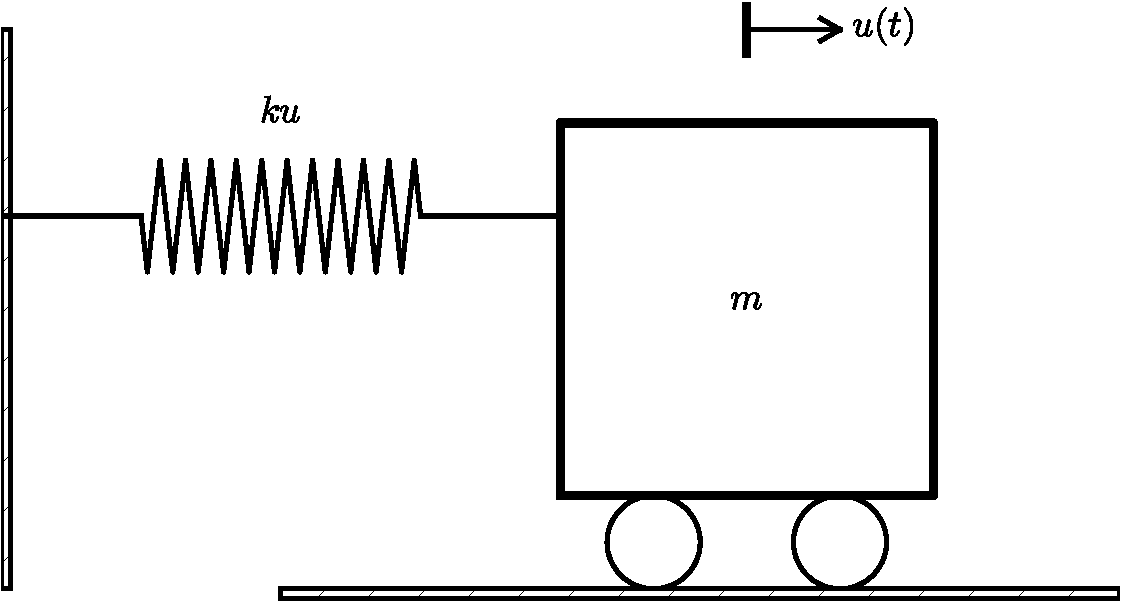
\includegraphics[width=0.7\linewidth]{fig-vib/oscillator_spring.pdf}}
  \caption{
  Simple oscillating mass. \label{vib:app:mass_spring:fig}
  }
\end{figure}
%\clearpage % flush figures vib:app:mass_spring:fig


The most fundamental mechanical vibration system is depicted in Figure~\ref{vib:app:mass_spring:fig}. A body with mass $m$ is attached to a
spring and can move horizontally without friction (in the wheels). The
position of the body is given by the vector $\rpos(t) = u(t)\ii$, where
$\ii$ is a unit vector in $x$ direction.
There is
only one force acting on the body: a spring force $\F_s =-ku\ii$, where
$k$ is a constant. The point $x=0$, where $u=0$, must therefore
correspond to the body's position
where the spring is neither extended nor compressed, so the force
vanishes.

The basic physical principle that governs the motion of the body is
Newton's second law of motion: $\F=m\acc$, where
$\F$ is the sum of forces on the body, $m$ is its mass, and $\acc=\ddot\rpos$
is the acceleration. We use the dot for differentiation with respect
to time, which is
usual in mechanics. Newton's second law simplifies here
to $-\F_s=m\ddot u\ii$, which translates to

\[ -ku = m\ddot u\tp\]
Two initial conditions are needed: $u(0)=I$, $\dot u(0)=V$.
The ODE problem is normally written as

\begin{equation}
m\ddot u + ku = 0,\quad u(0)=I,\ \dot u(0)=V\tp
\label{vib:app:mass_spring:eqx}
\end{equation}
It is
not uncommon to divide by $m$
and introduce the frequency $\omega = \sqrt{k/m}$:

\begin{equation}
\ddot u + \omega^2 u = 0,\quad u(0)=I,\  \dot u(0)=V\tp
\label{vib:app:mass_spring:equ}
\end{equation}
This is the model problem in the first part of this chapter, with the
small difference that we write the time derivative of $u$ with a dot
above, while we used $u^{\prime}$ and $u^{\prime\prime}$ in previous
parts of the document.

\index{DOF (degree of freedom)}

Since only one scalar mathematical quantity, $u(t)$, describes the
complete motion, we say that the mechanical system has one degree of freedom
(DOF).

\paragraph{Scaling.}
For numerical simulations it is very convenient to scale (\ref{vib:app:mass_spring:equ}) and thereby get rid of the problem of finding relevant values
for all the parameters $m$, $k$, $I$, and $V$.
Since the amplitude of the oscillations are dictated by $I$ and $V$
(or more precisely, $V/\omega$), we scale $u$ by $I$ (or $V/omega$ if
$I=0$):

\[ \bar u = \frac{u}{I},\quad \bar t = \frac{t}{t_c}\tp\]
The time scale $t_c$ is normally chosen as the inverse period $2\pi/\omega$ or
angular frequency $1/\omega$, most often as $t_c=1/\omega$.
Inserting the dimensionless quantities $\bar u$ and $\bar t$ in
(\ref{vib:app:mass_spring:equ}) results in the scaled problem

\[ \frac{d^2\bar u}{d\bar t^2} + \bar u = 0,\quad \bar u(0)=1,\ \frac{\bar u}{\bar t}(0)=\beta = \frac{V}{I\omega},\]
where $\beta$ is a dimensionless number. Any motion that starts from rest
($V=0$) is free of parameters in the scaled model!

\paragraph{The physics.}
The typical physics of the system in Figure~\ref{vib:app:mass_spring:fig} can
be described as follows.
Initially, we displace the body to some position $I$, say at rest
($V=0$). After releasing the body, the spring, which is extended, will
act with a force $-kI\ii$ and pull the body to the left. This force
causes an acceleration and therefore increases velocity. The body passes
the point $x=0$, where $u=0$,
and the spring will then be compressed and act with a
force $kx\ii$ against the motion and cause retardation. At some point,
the motion stops and the velocity is zero, before the spring force
$kx\ii$ accelerates the body in positive direction. The result is that
the body accelerates back and forth. As long as there is no friction
forces to damp the motion, the oscillations will continue forever.

\subsection{General mechanical vibrating system}
\label{vib:app:mass_gen}


\begin{figure}[!ht]  % vib:app:mass_gen:fig
  \centerline{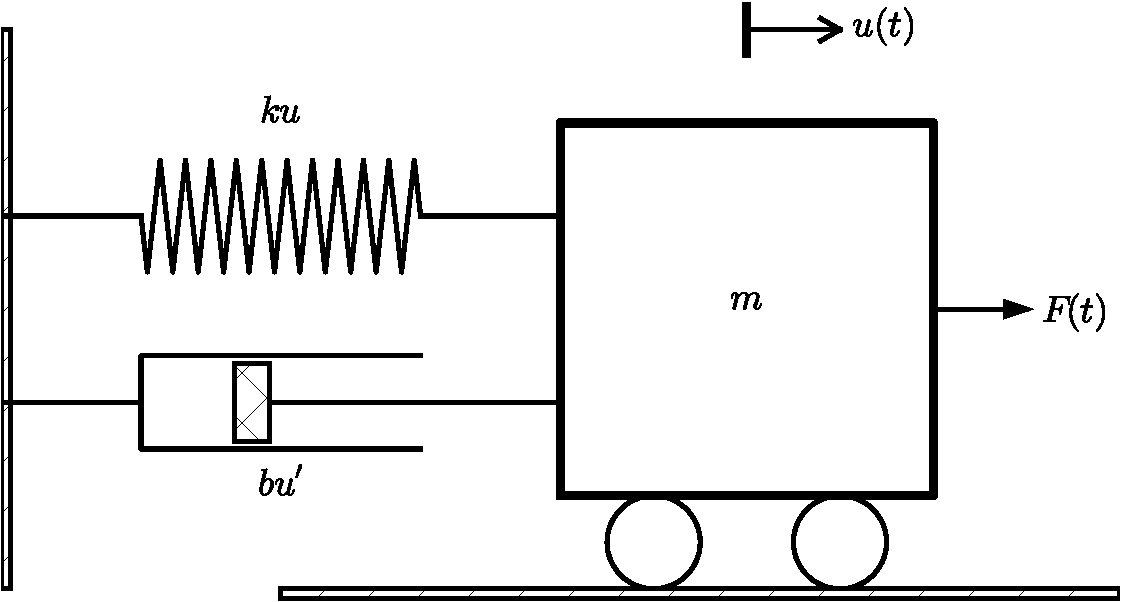
\includegraphics[width=0.7\linewidth]{fig-vib/oscillator_general.pdf}}
  \caption{
  General oscillating system. \label{vib:app:mass_gen:fig}
  }
\end{figure}
%\clearpage % flush figures vib:app:mass_gen:fig


The mechanical system in Figure~\ref{vib:app:mass_spring:fig} can easily be
extended to the more general system in Figure~\ref{vib:app:mass_gen:fig},
where the body is attached to a spring and a dashpot, and also subject
to an environmental force $F(t)\ii$. The system has still only one
degree of freedom since the body can only move back and forth parallel to
the $x$ axis. The spring force was linear, $\F_s=-ku\ii$,
in Section~\ref{vib:app:mass_spring}, but in more general cases it can
depend nonlinearly on the position. We therefore set $\F_s=s(u)\ii$.
The dashpot, which acts
as a damper, results in a force $\F_d$ that depends on the body's
velocity $\dot u$ and that always acts against the motion.
The mathematical model of the force is written $\F_d =f(\dot u)\ii$.
A positive $\dot u$ must result in a force acting in the positive $x$
direction.
Finally, we have the external environmental force $\F_e = F(t)\ii$.

Newton's second law of motion now involves three forces:

\[ F(t)\ii + f(\dot u)ii - s(u)\ii = m\ddot u \ii\tp\]
The common mathematical form of the ODE problem is

\begin{equation}
m\ddot u + f(\dot u) + s(u) = F(t),\quad u(0)=I,\ \dot u(0)=V\tp
\label{vib:app:mass_gen:equ}
\end{equation}
This is the generalized problem treated in the last part of the
present chapter, but with prime denoting the derivative instead of the dot.

The most common models for the spring and dashpot are linear: $f(\dot u)
=b\dot u$ with a constant $b\geq 0$, and $s(u)=ku$ for a constant $k$.

\paragraph{Scaling.}
A specific scaling requires specific choices of $f$, $s$, and $F$.
Suppose we have

\[ f(\dot u) = b|\dot u|\dot u,\quad s(u)=ku,\quad F(t)=A\sin(\phi t)\tp\]
We introduce dimensionless variables as usual, $\bar u = u/u_c$ and
$\bar t = t/t_c$. The scale $u_c$ depends both on the initial conditions
and $F$, but as time grows, the effect of the initial conditions die out
and $F$ will drive the motion. Inserting $\bar u$ and $\bar t$ in the
ODE gives

\[ m\frac{u_c}{t_c^2}\frac{d^2\bar u}{d\bar t^2}
+ b\frac{u_c^2}{t_c^2}\left\vert\frac{d\bar u}{d\bar t}\right\vert
\frac{d\bar u}{d\bar t} + ku_c\bar u = A\sin(\phi t_c\bar t)\tp\]
We divide by $u_c/t_c^2$ and demand the coefficients of the
$\bar u$ and the forcing term from $F(t)$ to have unit coefficients.
This leads to the scales

\[ t_c = \sqrt{\frac{m}{k}},\quad u_c = \frac{A}{k}\tp\]
The scaled ODE becomes

\begin{equation}
\frac{d^2\bar u}{d\bar t^2}
+ 2\beta\left\vert\frac{d\bar u}{d\bar t}\right\vert
\frac{d\bar u}{d\bar t} + \bar u = \sin(\gamma\bar t),
\label{vib:app:mass_gen:scaled}
\end{equation}
where there are two dimensionless numbers:

\[ \beta = \frac{Ab}{2mk},\quad\gamma =\phi\sqrt{\frac{m}{k}}\tp\]
The $\beta$ number measures the size of the damping term (relative to unity)
and is assumed to be small, basically because $b$ is small. The $\phi$
number is the ratio of the time scale of free vibrations and the time scale
of the forcing.
The scaled initial conditions have two other dimensionless numbers
as values:

\[ \bar u(0) = \frac{Ik}{A},\quad \frac{d\bar u}{d\bar t}=\frac{t_c}{u_c}V = \frac{V}{A}\sqrt{mk}\tp\]




\subsection{A sliding mass attached to a spring}
\label{vib:app:mass_sliding}

Consider a variant of the oscillating body in Section~\ref{vib:app:mass_spring}
and Figure~\ref{vib:app:mass_spring:fig}: the body rests on a flat
surface, and there is sliding friction between the body and the surface.
Figure~\ref{vib:app:mass_sliding:fig} depicts the problem.


\begin{figure}[!ht]  % vib:app:mass_sliding:fig
  \centerline{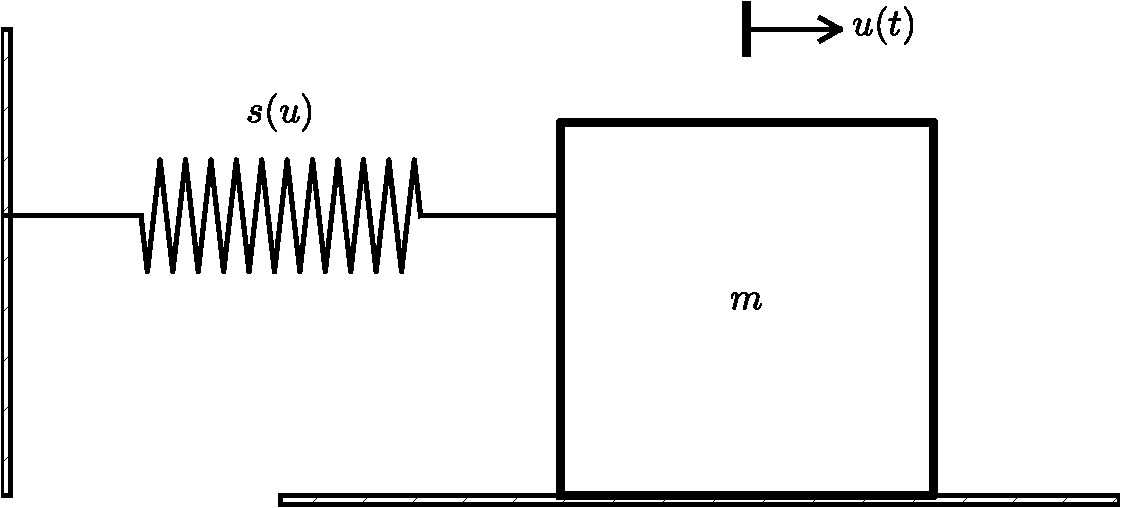
\includegraphics[width=0.7\linewidth]{fig-vib/oscillator_sliding.pdf}}
  \caption{
  Sketch of a body sliding on a surface. \label{vib:app:mass_sliding:fig}
  }
\end{figure}
%\clearpage % flush figures vib:app:mass_sliding:fig


The body is attached to a spring with spring force $-s(u)\ii$.
The friction force is proportional to the normal force on the surface,
$-mg\jj$, and given by $-f(\dot u)\ii$, where

\[ f(\dot u) = \left\lbrace\begin{array}{ll}
-\mu mg,& \dot u < 0,\\ 
\mu mg, & \dot u > 0,\\ 
0,      & \dot u=0
\end{array}\right.\]
Here, $\mu$ is a friction coefficient. With the signum function

\[ \mbox{sign(x)} = \left\lbrace\begin{array}{ll}
-1,& x < 0,\\ 
1, & x > 0,\\ 
0, & x=0
\end{array}\right.\]
we can simply write $f(\dot u) = \mu mg\,\hbox{sign}(\dot u)$
(the sign function is implemented by \texttt{numpy.sign}).

The equation of motion becomes

\begin{equation}
m\ddot u + \mu mg\hbox{sign}(\dot u) + s(u) = 0,\quad u(0)=I,\ \dot u(0)=V\tp
\label{vib:app:mass_sliding:equ}
\end{equation}

\subsection{A jumping washing machine}
\label{vib:app:washmach}

A washing machine is placed on four springs with efficient dampers.
If the machine contains just a few clothes, the circular motion of
the machine induces a sinusoidal external force and the machine will
jump up and down if the frequency of the external force is close to
the natural frequency of the machine and its spring-damper system.

\shortinlinecomment{hpl 10}{ Not finished. This is a good example on resonance. }{ Not finished. This is }



\subsection{Motion of a pendulum}
\label{vib:app:pendulum}

A classical problem in mechanics is the motion of a pendulum. We first
consider a \href{{https://en.wikipedia.org/wiki/Pendulum}}{simple pendulum}:
a small body of mass $m$ is attached to a massless wire and can oscillate back and forth
in the gravity field. Figure~\ref{vib:app:pendulum:fig_problem} shows
a sketch of the problem.


\begin{figure}[!ht]  % vib:app:pendulum:fig_problem
  \centerline{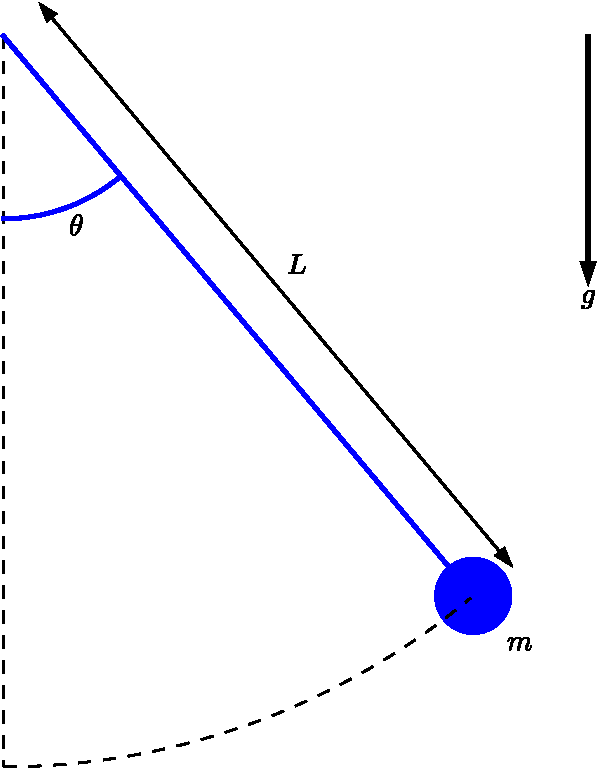
\includegraphics[width=0.4\linewidth]{fig-vib/pendulum_problem.pdf}}
  \caption{
  Sketch of a simple pendulum. \label{vib:app:pendulum:fig_problem}
  }
\end{figure}
%\clearpage % flush figures vib:app:pendulum:fig_problem


The motion is governed by Newton's 2nd law, so we need to find expressions
for the forces and the acceleration. Three forces on the body are
considered: an unknown force $S$ from the wire, the gravity force $mg$,
and an air resistance force, $\frac{1}{2}C_D\varrho A |v|v$,
hereafter called the drag force,
directed against the velocity of the body. Here, $C_D$ is a drag coefficient,
$\varrho$ is the density of air, $A$ is the cross section area of the body,
and $v$ is the velocity.

We introduce a coordinate system with polar coordinates and unit
vectors $\ir$ and $\ith$ as shown in Figure~\ref{vib:app:pendulum:fig_forces}.
The position of the center of mass of the body is

\[ \rpos(t) = x_0\ii + y_0\jj + L\ir,\]
where $\ii$ and $\jj$ are unit vectors in the corresponding Cartesian
coordinate system in the $x$ and $y$ directions, respectively. We have
that $\ir = \cos\theta\ii +\sin\theta\jj$.


\begin{figure}[!ht]  % vib:app:pendulum:fig_forces
  \centerline{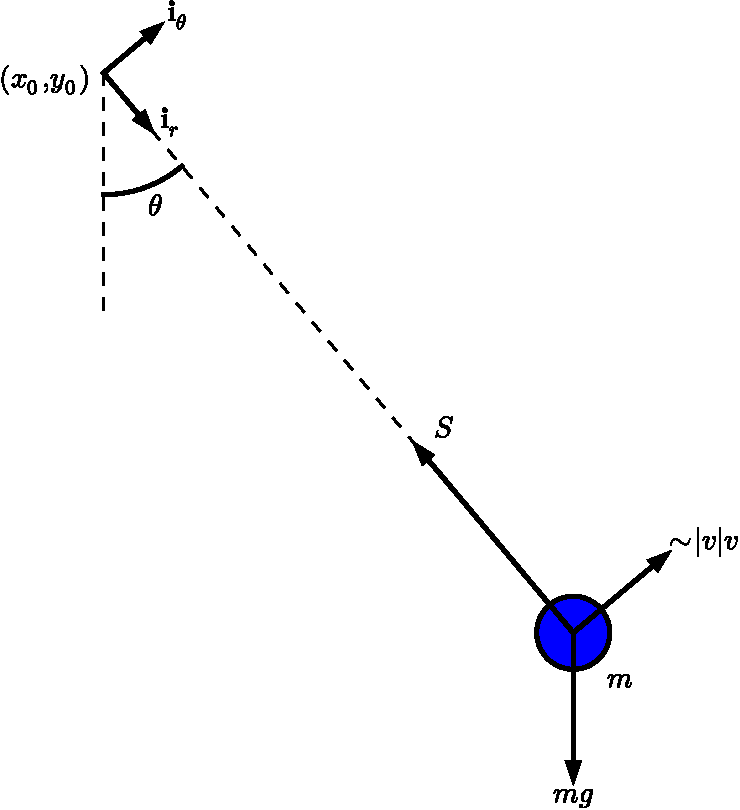
\includegraphics[width=0.5\linewidth]{fig-vib/pendulum_forces.pdf}}
  \caption{
  Forces acting on a simple pendulum. \label{vib:app:pendulum:fig_forces}
  }
\end{figure}
%\clearpage % flush figures vib:app:pendulum:fig_forces


The forces are now expressed as follows.

\begin{itemize}
 \item Wire force: $-S\ir$

 \item Gravity force: $-mg\jj = mg(-\sin\theta\ith + \cos\theta\ir)$

 \item Drag force: $-\frac{1}{2}C_D\varrho A |v|v\ith$
\end{itemize}

\noindent
Since a positive velocity means movement in the direction of $\ith$,
the drag force must be directed along $-\ith$.

The velocity of the body is found from $\rpos$:

\[ \v(t) = \dot\rpos (t) = \frac{d}{d\theta}(x_0\ii + y_0\jj + L\ir)\frac{d\theta}{dt} = L\dot\theta\ith,\]
since $\frac{d}{d\theta}\ir = \ith$. It follows that $v=|\v|=L\dot\theta$.
The acceleration is

\[ \acc(t) = \dot\v(r) = \frac{d}{dt}(L\dot\theta\ith)
= L\ddot\theta\ith + L\dot\theta\frac{d\ith}{d\theta}\dot\theta =
= L\ddot\theta\ith - L\dot\theta^2\ir,\]
since $\frac{d}{d\theta}\ith = -\ir$.

Newton's 2nd law of motion becomes

\[ -S\ir + mg(-\sin\theta\ith + \cos\theta\ir) -
\frac{1}{2}C_D\varrho AL^2|\dot\theta|\dot\theta\ith
= mL\ddot\theta\dot\theta\ith - L\dot\theta^2\ir,\]
leading to two component equations

\begin{align}
-S + mg\cos\theta &= -L\dot\theta^2,
\label{vib:app:pendulum:ir}\\ 
-mg\sin\theta - \frac{1}{2}C_D\varrho AL^2|\dot\theta|\dot\theta
&= mL\ddot\theta\tp
\label{vib:app:pendulum:ith}
\end{align}
From (\ref{vib:app:pendulum:ir}) we get an expression for
$S=mg\cos\theta + L\dot\theta^2$, and from (\ref{vib:app:pendulum:ith})
we get a differential equation for the angle $\theta(t)$. This latter
equation is ordered as

\begin{equation}
m\ddot\theta + + \frac{1}{2}C_D\varrho AL|\dot\theta|\dot\theta
+ \frac{mg}{L}\sin\theta = 0\tp
\label{vib:app:pendulum:thetaeq}
\end{equation}
Two initial conditions are needed: $\theta=\Theta$ and $\dot\theta = \Omega$.
Normally, the pendulum motion is started from rest, which means $\Omega =0$.

Equation (\ref{vib:app:pendulum:thetaeq}) fits the general model
used in (\ref{vib:ode2}) in Section~\ref{vib:model2} if we define
$u=\theta$, $f(u^{\prime}) = \frac{1}{2}C_D\varrho AL|\dot\theta|\dot\theta$,
$s(u) = L^{-1}mg\sin u$, and $F=0$.
If the body is a sphere with radius $R$, we can take $C_D=0.4$ and $A=\pi R^2$.

The motion of a compound or physical pendulum where the wire is a rod with
mass, can be modeled very similarly. The governing equation is
$I\acc = \bm{T}$ where $I$ is the moment of inertia of the entire body about
the point $(x_0,y_0)$, and $\bm{T}$ is the sum of moments of the forces
with respect to $(x_0,y_0)$. The vector equation reads

\[ \rpos\times(-S\ir + mg(-\sin\theta\ith + \cos\theta\ir) -
\frac{1}{2}C_D\varrho AL^2|\dot\theta|\dot\theta\ith)
= I(L\ddot\theta\dot\theta\ith - L\dot\theta^2\ir)\tp\]
The component equation in $\ith$ direction gives the equation of motion
for $\theta(t)$:

\begin{equation}
I\ddot\theta + \frac{1}{2}C_D\varrho AL^3|\dot\theta|\dot\theta
+ mgL\sin\theta = 0\tp
\label{vib:app:pendulum:thetaeq_physical}
\end{equation}

\shortinlinecomment{hpl 11}{ Scale the equations to arrive at the model problem with $\sin\theta$ spring. }{ Scale the equations to }

\subsection{Motion of an elastic pendulum}
\label{vib:app:pendulum_elastic}

Consider a pendulum as in Figure~\ref{vib:app:pendulum:fig_problem}, but
this time the wire is elastic. The length of the wire when it is not
stretched is $L_0$, while $L(t)$ is the stretched
length at time $t$ during the motion.

Stretching the elastic wire a distance $\Delta L$
gives rise to a spring force $k\Delta L$ in the opposite direction of the
stretching. Let $\normalvec$ be a unit normal vector along the wire
from the point $\rpos_0=(x_0,y_0)$ and in the direction of $\ith$,
see Figure~\ref{vib:app:pendulum:fig_forces} for definition of
$(x_0,y_0)$ and $\ith$. Obviously, we have $\normalvec=\ith$, but in
this modeling of an elastic pendulum we do not need polar coordinates.
Instead, it is more straightforward to develop the equation in
Cartesian coordinates.

A mathematical expression for $\normalvec$ is

\[ \normalvec = \frac{\rpos-\rpos_0}{L(t)},\]
where $L(t)=||\rpos-\rpos_0||$ is the current length of the elastic wire.
The position vector $\rpos$ in Cartesian coordinates reads
$\rpos(t) = x(t)\ii + y(t)\jj$, where $\ii$ and $\jj$ are unit vectors
in the $x$ and $y$ directions, respectively.
It is convenient to introduce the Cartesian components $n_x$ and $n_y$
of the normal vector:

\[ \normalvec = \frac{\rpos-\rpos_0}{L(t)} = \frac{x(t)-x_0}{L(t)}\ii + \frac{y(t)-y_0}{L(t)}\jj = n_x\ii + n_y\jj\tp\]

The stretch $\Delta L$ in the wire is

\[ \Delta t = L(t) - L_0\tp\]
The force in the wire is then $-S\normalvec=-k\Delta L\normalvec$.

The other forces are the gravity and the air resistance, just
as in Figure~\ref{vib:app:pendulum:fig_forces}. The main difference
is that we have a \emph{model} for $S$ in terms of the motion (as soon as
we have expressed $\Delta L$ by $\rpos$). For simplicity, we drop
the air resistance term (but Exercise~\ref{vib:exer:pendulum_elastic_drag}
asks you to include it).

Newton's second law of motion applied to the body now results in

\begin{equation}
m\ddot\rpos = -k(L-L_0)\normalvec - mg\jj
\label{vib:app:pendulum_elastic:eq1}
\end{equation}
The two components of
(\ref{vib:app:pendulum_elastic:eq1}) are

\begin{align}
\ddot x &= -\frac{k}{m}(L-L_0)n_x,\\ 
\label{vib:app:pendulum_elastic:eq2a} \\ 
\ddot y &= - \frac{k}{m}(L-L_0)n_y - g
\label{vib:app:pendulum_elastic:eq2b}\tp
\end{align}

\paragraph{Remarks about an elastic vs a non-elastic pendulum.}
Note that the derivation of the ODEs for an elastic pendulum is more
straightforward than for a classical, non-elastic pendulum,
since we avoid the details
with polar coordinates, but instead work with Newton's second law
directly in Cartesian coordinates. The reason why we can do this is that
the elastic pendulum undergoes a general two-dimensional motion where
all the forces are known or expressed as functions of $x(t)$ and $y(t)$,
such that we get two ordinary differential equations.
The motion of the non-elastic pendulum, on the other hand, is constrained:
the body has to move along a circular path, and the force $S$ in the
wire is unknown.

The non-elastic pendulum therefore leads to
a \emph{differential-algebraic} equation, i.e., ODEs for $x(t)$ and $y(t)$
combined with an extra constraint $(x-x_0)^2 + (y-y_0)^2 = L^2$
ensuring that the motion takes place along a circular path.
The extra constraint (equation) is compensated by an extra unknown force
$-S\normalvec$. Differential-algebraic equations are normally hard
to solve, especially with pen and paper.
Fortunately, for the non-elastic pendulum we can do a
trick: in polar coordinates the unknown force $S$ appears only in the
radial component of Newton's second law, while the unknown
degree of freedom for describing the motion, the angle $\theta(t)$,
is completely governed by the asimuthal component. This allows us to
decouple the unknowns $S$ and $\theta$. But this is a kind of trick and
not a widely applicable method. With an elastic pendulum we use straightforward
reasoning with Newton's 2nd law and arrive at a standard ODE problem that
(after scaling) is easy solve on a computer.

\paragraph{Initial conditions.}
What is the initial position of the body? We imagine that first the
pendulum hangs in equilibrium in its vertical position, and then it is
displaced an angle $\Theta$. The equilibrium position is governed
by the ODEs with the accelerations set to zero.
The $x$ component leads to $x(t)=x_0$, while the $y$ component gives

\[ 0 = - \frac{k}{m}(L-L_0)n_y - g = \frac{k}{m}(L(0)-L_0) - g\quad\Rightarrow\quad
L(0) = L_0 + mg/k,\]
since $n_y=-11$ in this position. The corresponding $y$ value is then
from $n_y=-1$:

\[ y(t) = y_0 - L(0) = y_0 - (L_0 + mg/k)\tp\]
Let us now choose $(x_0,y_0)$ such that the body is at the origin
in the equilibrium position:

\[ x_0 =0,\quad y_0 = L_0 + mg/k\tp\]

Displacing the body an angle $\Theta$ to the right leads to the
initial position

\[ x(0)=(L_0+mg/k)\sin\Theta,\quad y(0)=(L_0+mg/k)(1-\cos\Theta)\tp\]
The initial velocities can be set to zero: $x'(0)=y'(0)=0$.

\paragraph{The complete ODE problem.}
We can summarize all the equations as follows:

\begin{align*}
\ddot x &= -\frac{k}{m}(L-L_0)n_x,
\\ 
\ddot y &= -\frac{k}{m}(L-L_0)n_y - g,
\\ 
L &= \sqrt{(x-x_0)^2 + (y-y_0)^2},
\\ 
n_x &= \frac{x-x_0}{L},
\\ 
n_y &= \frac{y-y_0}{L},
\\ 
x(0) &= (L_0+mg/k)\sin\Theta,
\\ 
x'(0) &= 0,
\\ 
y(0) & =(L_0+mg/k)(1-\cos\Theta),
\\ 
y'(0) &= 0\tp
\end{align*}
We insert $n_x$ and $n_y$  in the ODEs:

\begin{align}
\ddot x &= -\frac{k}{m}\left(1 -\frac{L_0}{L}\right)(x-x_0),
\label{vib:app:pendulum_elastic:x}\\ 
\ddot y &= -\frac{k}{m}\left(1 -\frac{L_0}{L}\right)(y-y_0) - g,
\label{vib:app:pendulum_elastic:y}\\ 
L &= \sqrt{(x-x_0)^2 + (y-y_0)^2},
\label{vib:app:pendulum_elastic:L}\\ 
x(0) &= (L_0+mg/k)\sin\Theta,
\label{vib:app:pendulum_elastic:x0}\\ 
x'(0) &= 0,
\label{vib:app:pendulum_elastic:vx0}\\ 
y(0) & =(L_0+mg/k)(1-\cos\Theta),
\label{vib:app:pendulum_elastic:y0}\\ 
y'(0) &= 0\tp
\label{vib:app:pendulum_elastic:vy0}
\end{align}

\paragraph{Scaling.}
The elastic pendulum model can be used to study both an elastic pendulum
and a classic, non-elastic pendulum. The latter problem is obtained
by letting $k\rightarrow\infty$. Unfortunately,
a serious problem with the ODEs
(\ref{vib:app:pendulum_elastic:x})-(\ref{vib:app:pendulum_elastic:y}) is that for large $k$, we have a very large factor $k/m$ multiplied by a
very small number $1-L_0/L$, since for large $k$, $L\approx L_0$ (very
small deformations of the wire). The product is subject to
significant round-off errors for many relevant physical values of
the parameters. To circumvent the problem, we introduce a scaling. This
will also remove physical parameters from the problem such that we end
up with only one dimensionless parameter,
closely related to the elasticity of the wire. Simulations can then be
done by setting just this dimensionless parameter.

The characteristic length can be taken such that in equilibrium, the
scaled length is unity, i.e., the characteristic length is $L_0+mg/k$:

\[ \bar x = \frac{x}{L_0+mg/k},\quad \bar y = \frac{y}{L_0+mg/k}\tp\]
We must then also work with the scaled length $\bar L = L/(L_0+mg/k)$.

Introducing $\bar t=t/t_c$, where $t_c$ is a characteristic time we
have to decide upon later, one gets

\begin{align*}
\frac{d^2\bar x}{d\bar t^2} &=
-t_c^2\frac{k}{m}\left(1 -\frac{L_0}{L_0+mg/k}\frac{1}{\bar L}\right)\bar x,\\ 
\frac{d^2\bar y}{d\bar t^2} &=
-t_c^2\frac{k}{m}\left(1 -\frac{L_0}{L_0+mg/k}\frac{1}{\bar L}\right)(\bar y-1)
-t_c^2\frac{g}{L_0 + mg/k},\\ 
\bar L &= \sqrt{\bar x^2 + (\bar y-1)^2},\\ 
\bar x(0) &= \sin\Theta,\\ 
\bar x'(0) &= 0,\\ 
\bar y(0) & = 1 - \cos\Theta,\\ 
\bar y'(0) &= 0\tp
\end{align*}
For a non-elastic pendulum with small angles, we know that the
frequency of the oscillations are $\omega = \sqrt{L/g}$. It is therefore
natural to choose a similar expression here, either the length in
the equilibrium position,

\[ t_c^2 = \frac{L_0+mg/k}{g}\tp\]
or simply the unstretched length,

\[ t_c^2 = \frac{L_0}{g}\tp\]
These quantities are not very different (since the elastic model
is valid only for quite small elongations), so we take the latter as it is
the simplest one.

The ODEs become

\begin{align*}
\frac{d^2\bar x}{d\bar t^2} &=
-\frac{L_0k}{mg}\left(1 -\frac{L_0}{L_0+mg/k}\frac{1}{\bar L}\right)\bar x,\\ 
\frac{d^2\bar y}{d\bar t^2} &=
-\frac{L_0k}{mg}\left(1 -\frac{L_0}{L_0+mg/k}\frac{1}{\bar L}\right)(\bar y-1)
-\frac{L_0}{L_0 + mg/k},\\ 
\bar L &= \sqrt{\bar x^2 + (\bar y-1)^2}\tp
\end{align*}
We can now identify a dimensionless number

\[ \beta = \frac{L_0}{L_0 + mg/k} = \frac{1}{1+\frac{mg}{L_0k}},\]
which is the ratio of the unstretched length and the
stretched length in equilibrium. The non-elastic pendulum will have
$\beta =1$ ($k\rightarrow\infty$).
With $\beta$ the ODEs read

\begin{align}
\frac{d^2\bar x}{d\bar t^2} &=
-\frac{\beta}{1-\beta}\left(1- \frac{\beta}{\bar L}\right)\bar x,
\label{vib:app:pendulum_elastic:x:s}\\ 
\frac{d^2\bar y}{d\bar t^2} &=
-\frac{\beta}{1-\beta}\left(1- \frac{\beta}{\bar L}\right)(\bar y-1)
-\beta,
\label{vib:app:pendulum_elastic:y:s}\\ 
\bar L &= \sqrt{\bar x^2 + (\bar y-1)^2},
\label{vib:app:pendulum_elastic:L:s}\\ 
\bar x(0) &= (1+\epsilon)\sin\Theta,
\label{vib:app:pendulum_elastic:x0:s}\\ 
\frac{d\bar x}{d\bar t}(0) &= 0,
\label{vib:app:pendulum_elastic:vx0:s}\\ 
\bar y(0) &= 1 - (1+\epsilon)\cos\Theta,
\label{vib:app:pendulum_elastic:y0:s}\\ 
\frac{d\bar y}{d\bar t}(0) &= 0,
\label{vib:app:pendulum_elastic:vy0:s}
\end{align}
We have here added a parameter $\epsilon$, which is an additional
downward stretch of the wire at $t=0$. This parameter makes it possible
to do a desired test: vertical oscillations of the pendulum. Without
$\epsilon$, starting the motion from $(0,0)$ with zero velocity will
result in $x=y=0$ for all times (also a good test!), but with
an initial stretch so the body's position is $(0,\epsilon)$, we
will have oscillatory vertical motion with amplitude $\epsilon$ (see
Exercise~\ref{vib:exer:pendulum_elastic}).

\paragraph{Remark on the non-elastic limit.}
We immediately see that as $k\rightarrow\infty$ (i.e., we obtain a non-elastic
pendulum), $\beta\rightarrow 1$, $\bar L\rightarrow 1$, and we have
very small values $1-\beta\bar L^{-1}$ divided by very small values
$1-\beta$ in the ODEs. However, it turns out that we can set $\beta$
very close to one and obtain a path of the body that within the visual
accuracy of a plot does not show any elastic oscillations.
(Should the division of very small values become a problem, one can
study the limit by L'Hospital's rule:

\[ \lim_{\beta\rightarrow 1}\frac{1 - \beta \bar L^{-1}}{1-\beta}
= \frac{1}{\bar L},\]
and use the limit $\bar L^{-1}$ in the ODEs for $\beta$ values very
close to 1.)


\subsection{Bouncing ball}
\label{vib:app:bouncing_ball}

A bouncing ball is a body in free vertically fall until it impacts the
ground. During the impact, some kinetic energy is lost, and a new
motion upwards with reduced velocity starts.  At some point the
velocity close to the ground is so small that the ball is considered
to be finally at rest.

The motion of the ball falling in air is governed by Newton's second
law $F=ma$, where $a$ is the acceleration of the body, $m$ is the mass,
and $F$ is the sum of all forces. Here, we neglect the air resistance
so that gravity $-mg$ is the only force. The height of the ball is
denoted by $h$ and $v$ is the velocity. The relations between $h$, $v$, and
$a$,

\[ h'(t)= v(t),\quad v'(t) = a(t),\]
combined with Newton's second law gives the ODE model

\begin{equation}
h^{\prime\prime}(t) = -g,
\label{vib:app:bouncing:ball:h2eq}
\end{equation}
or expressed alternatively as a system of first-order equations:

\begin{align}
v'(t) &= -g,
\label{vib:app:bouncing:ball:veq} \\ 
h'(t) &= v(t)\tp
\label{vib:app:bouncing:ball:heq}
\end{align}
These equations govern the motion as long as the ball is away from
the ground by a small distance $\epsilon_h > 0$. When $h<\epsilon_h$,
we have two cases.

\begin{enumerate}
\item The ball impacts the ground, recognized by a sufficiently large negative
   velocity ($v<-\epsilon_v$). The velocity then changes sign and is
   reduced by a factor $C_R$, known as the \href{{http://en.wikipedia.org/wiki/Coefficient_of_restitution}}{coefficient of restitution}.
   For plotting purposes, one may set $h=0$.

\item The motion stops, recognized by a sufficiently small velocity
   ($|v|<\epsilon_v$) close to the ground.
\end{enumerate}

\noindent
\subsection{Electric circuits}

Although the term ``mechanical vibrations'' is used in the present
document, we must mention that the same type of equations arise
when modeling electric circuits.
The current $I(t)$ in a
circuit with an inductor with inductance $L$, a capacitor with
capacitance $C$, and overall resistance $R$, is governed by

\begin{equation}
\ddot I + \frac{R}{L}\dot I + \frac{1}{LC}I = \dot V(t),
\end{equation}
where $V(t)$ is the voltage source powering the circuit.
This equation has the same form as the general model considered in
Section refref{vib:model2} if we set $u=I$, $f(u^{\prime}=bu^{\prime}$
and define $b=R/L$, $s(u) = L^{-1}C^{-1}u$, and $F(t)=\dot V(t)$.


\section{Exercises}



% --- begin exercise ---
\begin{doconceexercise}
\refstepcounter{doconceexercisecounter}

\subsection*{Exercise \thedoconceexercisecounter: Simulate resonance}

\label{vib:exer:resonance}

\index{resonance}

We consider the scaled ODE model
(\ref{vib:app:mass_gen:scaled}) from Section~\ref{vib:app:mass_gen}.
After scaling, the amplitude of $u$ will have a size about unity
as time grows and the effect of the initial conditions die out due
to damping. However, as $\gamma\rightarrow 1$, the amplitude of $u$
increases, especially if $\beta$ is small. This effect is called
\emph{resonance}. The purpose of this exercise is to explore resonance.


\subex{a)}
Figure out how the \texttt{solver} function in \texttt{vib.py} can be called
for the scaled ODE (\ref{vib:app:mass_gen:scaled}).


% removed !bsol ... !esol environment (because of the command-line option --without_solutions)

\subex{b)}
Run $\gamma =5, 1.5, 1.1, 1$ for $\beta=0.005, 0.05, 0.2$.
For each $\beta$ value, present an image with plots of $u(t)$ for
the four $\gamma$ values.


% removed !bsol ... !esol environment (because of the command-line option --without_solutions)

\noindent Filename: \texttt{resonance}.

\end{doconceexercise}
% --- end exercise ---




% --- begin exercise ---
\begin{doconceexercise}
\refstepcounter{doconceexercisecounter}

\subsection*{Exercise \thedoconceexercisecounter: Simulate oscillations of a sliding box}

\label{vib:exer:sliding_box}

Consider a sliding box on a flat surface as modeled in Section~\ref{vib:app:mass_sliding}. As spring force we choose the nonlinear
formula

\[ s(u) = \frac{k}{\alpha}\tanh(\alpha u) = ku + \frac{1}{3}\alpha^2 ku^3 + \frac{2}{15}\alpha^4 k u^5 + \Oof{u^6}\tp\]


\subex{a)}
Plot $g(u)=\alpha^{-1}\tanh(\alpha u)$ for various values of $\alpha$.
Assume $u\in [-1,1]$.


% removed !bsol ... !esol environment (because of the command-line option --without_solutions)

\subex{b)}
Scale the equations using $I$ as scale for $u$ and $m/k$ as
time scale.


% removed !bsol ... !esol environment (because of the command-line option --without_solutions)

\subex{c)}
Implement the scaled model in b). Run it for some values of
the dimensionless parameters.


% removed !bsol ... !esol environment (because of the command-line option --without_solutions)

\noindent Filename: \Verb!sliding_box!.

\end{doconceexercise}
% --- end exercise ---




% --- begin exercise ---
\begin{doconceexercise}
\refstepcounter{doconceexercisecounter}

\subsection*{Exercise \thedoconceexercisecounter: Simulate a bouncing ball}

\label{vib:exer:bouncing:ball}

Section~\ref{vib:app:bouncing_ball} presents a model for a bouncing
ball.
Choose one of the two ODE formulation, (\ref{vib:app:bouncing:ball:h2eq}) or
(\ref{vib:app:bouncing:ball:veq})-(\ref{vib:app:bouncing:ball:heq}),
and simulate the motion of a bouncing ball. Plot $h(t)$. Think about how to
plot $v(t)$.

% --- begin hint in exercise ---

\paragraph{Hint.}
A naive implementation may get stuck in repeated impacts for large time
step sizes. To avoid this situation, one can introduce a state
variable that holds the mode of the motion: free fall, impact, or rest.
Two consecutive impacts imply that the motion has stopped.

% --- end hint in exercise ---


% removed !bsol ... !esol environment (because of the command-line option --without_solutions)
\noindent Filename: \Verb!bouncing_ball!.

\end{doconceexercise}
% --- end exercise ---




% --- begin exercise ---
\begin{doconceexercise}
\refstepcounter{doconceexercisecounter}

\subsection*{Exercise \thedoconceexercisecounter: Simulate an elastic pendulum}

\label{vib:exer:pendulum_elastic}

Section~\ref{vib:app:pendulum_elastic} describes a model for an elastic
pendulum, resulting in a system of two ODEs. The purpose of this
exercise is to implement the scaled model, test the software, and
generalize the model.


\subex{a)}
Write a function \texttt{simulate}
that can simulate an elastic pendulum using the scaled model.
The function should have the following arguments:

\begin{cod}{cbg_blue1}\begin{Verbatim}[numbers=none,fontsize=\fontsize{9pt}{9pt},baselinestretch=0.95,xleftmargin=2mm]
def simulate(
    beta=0.9,                 # dimensionless parameter
    Theta=30,                 # initial angle in degrees
    epsilon=0,                # initial stretch of wire
    num_periods=6,            # simulate for num_periods
    time_steps_per_period=60, # time step resolution
    plot=True,                # make plots or not
    ):
\end{Verbatim}
\end{cod}
\noindent
To set the total simulation time and the time step, we
use our knowledge of the scaled, classical, non-elastic pendulum:
$u^{\prime\prime} + u = 0$, with solution
$u = \Theta\cos \bar t$.
The period of these oscillations is $P=2\pi$
and the frequency is unity. The time
for simulation is taken as \Verb!num_periods! times $P$. The time step
is set as $P$ divided by \Verb!time_steps_per_period!.

The \texttt{simulate} function should return the arrays of
$x$, $y$, $\theta$, and $t$, where $\theta = \tan^{-1}(x/(1-y))$ is
the angular displacement of the elastic pendulum corresponding to the
position $(x,y)$.

If \texttt{plot} is \texttt{True}, make a plot of $\bar y(\bar t)$
versus $\bar x(\bar t)$, i.e., the physical motion
of the mass at $(\bar x,\bar y)$. Use the equal aspect ratio on the axis
such that we get a physically correct picture of the motion. Also
make a plot of $\theta(\bar t)$, where $\theta$ is measured in degrees.
If $\Theta < 10$ degrees, add a plot that compares the solutions of
the scaled, classical, non-elastic pendulum and the elastic pendulum
($\theta(t)$).

Although the mathematics here employs a bar over scaled quantities, the
code should feature plain names \texttt{x} for $\bar x$, \texttt{y} for $\bar y$, and
\texttt{t} for $\bar t$ (rather than \Verb!x_bar!, etc.). These variable names make
the code easier to read and compare with the mathematics.

% --- begin hint in exercise ---

\paragraph{Hint 1.}
Equal aspect ratio is set by \Verb!plt.gca().set_aspect('equal')! in
Matplotlib (\texttt{import matplotlib.pyplot as plt})
and by \texttt{plot(..., daspect=[1,1,1], daspectmode='equal')}
in SciTools (\texttt{import scitools.std as plt}).

% --- end hint in exercise ---

% --- begin hint in exercise ---

\paragraph{Hint 2.}
If you want to use Odespy to solve the equations, order the ODEs
like $\dot \bar x, \bar x, \dot\bar y,\bar y$ such that the Euler-Cromer
scheme can (also) be used (\texttt{odespy.EulerCromer}).

% --- end hint in exercise ---


% removed !bsol ... !esol environment (because of the command-line option --without_solutions)

\subex{b)}
Write a test function for testing that $\Theta=0$ and $\epsilon=0$
gives $x=y=0$ for all times.


% removed !bsol ... !esol environment (because of the command-line option --without_solutions)

\subex{c)}
Write another test function for checking that the pure vertical
motion of the elastic pendulum is correct.
Start with simplifying the ODEs for pure vertical motion and show that
$\bar y(\bar t)$ fulfills a vibration equation with
frequency $\sqrt{\beta/(1-\beta)}$. Set up the exact solution.

Write a test function that
uses this special case to verify the \texttt{simulate} function. There will
be numerical approximation errors present in the results from
\texttt{simulate} so you have to believe in correct results and set a
(low) tolerance that corresponds to the computed maximum error.
Use a small $\Delta t$ to obtain a small numerical approximation error.


% removed !bsol ... !esol environment (because of the command-line option --without_solutions)

\subex{d)}
Make a function \texttt{demo(beta, Theta)} for simulating an elastic pendulum with a
given $\beta$ parameter and initial angle $\Theta$. Use 600 time steps
per period to get every accurate results, and simulate for 3 periods.


% removed !bsol ... !esol environment (because of the command-line option --without_solutions)

\noindent Filename: \Verb!elastic_pendulum!.

\end{doconceexercise}
% --- end exercise ---




% --- begin exercise ---
\begin{doconceexercise}
\refstepcounter{doconceexercisecounter}

\subsection*{Exercise \thedoconceexercisecounter: Simulate an elastic pendulum with air resistance}

\label{vib:exer:pendulum_elastic_drag}

This is a continuation Exercise~\ref{vib:exer:pendulum_elastic_drag}.
Air resistance on the body with mass $m$ can be modeled by the
force $-\frac{1}{2}\varrho C_D A|\v|\v$,
where $C_D$ is a drag coefficient (0.2 for a sphere), $\varrho$
is the density of air (1.2 $\hbox{kg }\,{\hbox{m}}^{-3}$), $A$ is the
cross section area ($A=\pi R^2$ for a sphere, where $R$ is the radius),
and $\v$ is the velocity of the body.
Include air resistance in the original model, scale the model,
write a function \Verb!simulate_drag! that is a copy of the \texttt{simulate}
function from Exercise~\ref{vib:exer:pendulum_elastic_drag}, but with the
new ODEs included, and show plots of how air resistance
influences the motion.


% removed !bsol ... !esol environment (because of the command-line option --without_solutions)
\noindent Filename: \Verb!elastic_pendulum_drag!.

% Closing remarks for this Exercise

\paragraph{Remarks.}
Test functions are challenging to construct for the problem with
air resistance. You can reuse the tests from
Exercise~\ref{vib:exer:pendulum_elastic_drag} for \Verb!simulate_drag!,
but these tests does not verify the new terms arising from air
resistance.





% in vb_odespy examples: add 20 RK4 1000 to show RK4 in the long run

% mu'' + bu' + ku = F(t)
% set up analytical solution for reference
% compare for F = sin qt, demonstrate resonance by having
% F = sin q t and q = piecewise constant in time with four
% levels: 0.1, 0.75 1, 1.25, 2 of the resonance frequency,
% make each platou act for a while to see the effect

% mu'' + bu' + s(u) = F(t) as exercise, pendulum
% mu'' + f(x) + s() = F(t) via odespy RK4

% odespy: ForwardBackward on a 2n system? Need special formula for first
% step to ensure dt^2 accuracy there.

% apps: planet around a star, box horizontal and vertical, bumpy,
% jumping washing machine, pendulum, moored ship, look to Irgens
\end{doconceexercise}
% --- end exercise ---




\bibliographystyle{plain}
\bibliography{../papers}

% ------------------- end of main content ---------------

% #ifdef PREAMBLE
\cleardoublepage\phantomsection  % trick to get correct link to Index
\printindex

\end{document}
% #endif

